%Version 3.1 December 2024 template; compile with the official sn-jnl.cls
\documentclass[pdflatex,sn-mathphys-num,iicol]{sn-jnl}
\usepackage{graphicx}\usepackage{multirow}\usepackage{amsmath,amssymb,amsfonts}\usepackage{amsthm}
\usepackage{mathrsfs}\usepackage{xcolor}\usepackage{textcomp}\usepackage{booktabs}\usepackage{url}
\usepackage{algorithm}\usepackage{algorithmicx}\usepackage{algpseudocode}
\theoremstyle{thmstyleone}
\newtheorem{proposition}{Proposition}
\newtheorem{theorem}[proposition]{Theorem}
\newtheorem{lemma}[proposition]{Lemma}
\newtheorem{corollary}[proposition]{Corollary}
\theoremstyle{thmstyletwo}
\newtheorem{remark}{Remark}
\newtheorem{assumption}{Assumption}
\theoremstyle{thmstylethree}
\newtheorem{definition}{Definition}
\raggedbottom
\newcommand{\SIref}[1]{\ifcsname siref@#1\endcsname\csname siref@#1\endcsname\else\textbf{??}\fi}
\newcommand{\Mref}[1]{\ifcsname mref@#1\endcsname\csname mref@#1\endcsname\else\textbf{??}\fi}
\renewcommand{\thesection}{S\arabic{section}}
\renewcommand{\thesubsection}{\thesection.\arabic{subsection}}
\renewcommand{\thetable}{S\arabic{table}}
\renewcommand{\thefigure}{S\arabic{figure}}
\renewcommand{\theequation}{S\arabic{equation}}
\renewcommand{\theproposition}{S\arabic{proposition}}
\renewcommand{\theremark}{S\arabic{remark}}
\renewcommand{\theassumption}{S\arabic{assumption}}
\renewcommand{\thedefinition}{S\arabic{definition}}
\makeatletter
\expandafter\gdef\csname siref@app:data\endcsname{S9}
\expandafter\gdef\csname siref@cor:uniform\endcsname{S11}
\expandafter\gdef\csname siref@eq:alloc-loss\endcsname{S7}
\expandafter\gdef\csname siref@eq:deff-err\endcsname{S9}
\expandafter\gdef\csname siref@eq:deff-lambda\endcsname{S11}
\expandafter\gdef\csname siref@eq:deff-mixed\endcsname{S12}
\expandafter\gdef\csname siref@eq:deff-sandwich\endcsname{S13}
\expandafter\gdef\csname siref@eq:deff-small\endcsname{S10}
\expandafter\gdef\csname siref@eq:deff-tpr\endcsname{S8}
\expandafter\gdef\csname siref@eq:dif-closed\endcsname{S4}
\expandafter\gdef\csname siref@eq:dif-misspec\endcsname{S5}
\expandafter\gdef\csname siref@eq:floor\endcsname{S6}
\expandafter\gdef\csname siref@eq:proxy-loss\endcsname{S14}
\expandafter\gdef\csname siref@eq:resid-forms\endcsname{S2}
\expandafter\gdef\csname siref@eq:resid-moments\endcsname{S3}
\expandafter\gdef\csname siref@eq:si-ingredients\endcsname{S15}
\expandafter\gdef\csname siref@eq:slut-a\endcsname{S16}
\expandafter\gdef\csname siref@eq:slut-b\endcsname{S17}
\expandafter\gdef\csname siref@eq:taylor\endcsname{S1}
\expandafter\gdef\csname siref@fig:abl-coverage\endcsname{S7}
\expandafter\gdef\csname siref@fig:abl-models\endcsname{S6}
\expandafter\gdef\csname siref@fig:abl-proxy\endcsname{S8}
\expandafter\gdef\csname siref@fig:base-efficiency\endcsname{S5}
\expandafter\gdef\csname siref@fig:sim-dif-real\endcsname{S3}
\expandafter\gdef\csname siref@fig:sim-dif-synth\endcsname{S4}
\expandafter\gdef\csname siref@fig:sim-real\endcsname{S1}
\expandafter\gdef\csname siref@fig:sim-rho\endcsname{S2}
\expandafter\gdef\csname siref@lem:crit\endcsname{S13}
\expandafter\gdef\csname siref@lem:slutsky\endcsname{S10}
\expandafter\gdef\csname siref@lem:strat-clt\endcsname{S12}
\expandafter\gdef\csname siref@prop:alloc-dif\endcsname{S7}
\expandafter\gdef\csname siref@prop:deff\endcsname{S8}
\expandafter\gdef\csname siref@prop:dif-closed\endcsname{S4}
\expandafter\gdef\csname siref@prop:dif-lambda\endcsname{S6}
\expandafter\gdef\csname siref@prop:dif-proxy\endcsname{S5}
\expandafter\gdef\csname siref@prop:dif-var-ext\endcsname{S3}
\expandafter\gdef\csname siref@prop:eo\endcsname{S15}
\expandafter\gdef\csname siref@prop:lemma-cov\endcsname{S1}
\expandafter\gdef\csname siref@prop:proxy\endcsname{S9}
\expandafter\gdef\csname siref@prop:residual\endcsname{S2}
\expandafter\gdef\csname siref@rem:zero-var-ext\endcsname{S1}
\expandafter\gdef\csname siref@sec:app-ablations\endcsname{S8}
\expandafter\gdef\csname siref@sec:sim-dif\endcsname{S5.4}
\expandafter\gdef\csname siref@sec:sim-proxy\endcsname{S5.3}
\expandafter\gdef\csname siref@sec:sim-real\endcsname{S5.1}
\expandafter\gdef\csname siref@sec:sim-synth\endcsname{S5.2}
\expandafter\gdef\csname siref@sec:simulation\endcsname{S5}
\expandafter\gdef\csname siref@sec:theory-proofs\endcsname{S1}
\expandafter\gdef\csname siref@si:ablation-tables\endcsname{S8}
\expandafter\gdef\csname siref@si:ablations\endcsname{S7}
\expandafter\gdef\csname siref@si:baselines\endcsname{S6}
\expandafter\gdef\csname siref@si:proofs\endcsname{S1}
\expandafter\gdef\csname siref@si:testing\endcsname{S3}
\expandafter\gdef\csname siref@si:testing-are\endcsname{S3.3}
\expandafter\gdef\csname siref@si:testing-clt\endcsname{S3.4}
\expandafter\gdef\csname siref@si:testing-crit\endcsname{S3.6}
\expandafter\gdef\csname siref@si:testing-design\endcsname{S3.9}
\expandafter\gdef\csname siref@si:testing-eo\endcsname{S3.12}
\expandafter\gdef\csname siref@si:testing-eo-stmt\endcsname{S3.11}
\expandafter\gdef\csname siref@si:testing-extra\endcsname{S3.10}
\expandafter\gdef\csname siref@si:testing-fwer\endcsname{S3.7}
\expandafter\gdef\csname siref@si:testing-joint\endcsname{S3.5}
\expandafter\gdef\csname siref@si:testing-pop\endcsname{S3.8}
\expandafter\gdef\csname siref@si:testing-sim\endcsname{S4}
\expandafter\gdef\csname siref@si:testing-size\endcsname{S3.2}
\expandafter\gdef\csname siref@si:testing-slutsky\endcsname{S3.1}
\expandafter\gdef\csname siref@si:theory-alloc\endcsname{S2.7}
\expandafter\gdef\csname siref@si:theory-deff\endcsname{S2.8}
\expandafter\gdef\csname siref@si:theory-deff-ratio\endcsname{S2.3}
\expandafter\gdef\csname siref@si:theory-dif\endcsname{S2.2}
\expandafter\gdef\csname siref@si:theory-dif-proxy\endcsname{S2.4}
\expandafter\gdef\csname siref@si:theory-extra\endcsname{S2}
\expandafter\gdef\csname siref@si:theory-floor\endcsname{S2.6}
\expandafter\gdef\csname siref@si:theory-lambda\endcsname{S2.5}
\expandafter\gdef\csname siref@si:theory-proxy\endcsname{S2.9}
\expandafter\gdef\csname siref@si:theory-resid\endcsname{S2.1}
\expandafter\gdef\csname siref@tab:abl-app-cov\endcsname{S23}
\expandafter\gdef\csname siref@tab:abl-app-eff-design\endcsname{S19}
\expandafter\gdef\csname siref@tab:abl-app-eff-proxy\endcsname{S20}
\expandafter\gdef\csname siref@tab:abl-app-eff-proxy-ht\endcsname{S21}
\expandafter\gdef\csname siref@tab:abl-app-eff-tuned\endcsname{S22}
\expandafter\gdef\csname siref@tab:abl-app-eo\endcsname{S25}
\expandafter\gdef\csname siref@tab:abl-app-models\endcsname{S26}
\expandafter\gdef\csname siref@tab:abl-app-width\endcsname{S24}
\expandafter\gdef\csname siref@tab:abl-eo\endcsname{S18}
\expandafter\gdef\csname siref@tab:abl-lambda\endcsname{S27}
\expandafter\gdef\csname siref@tab:abl-models\endcsname{S17}
\expandafter\gdef\csname siref@tab:abl-proxy\endcsname{S16}
\expandafter\gdef\csname siref@tab:base-setting\endcsname{S15}
\expandafter\gdef\csname siref@tab:sim-dif-real\endcsname{S13}
\expandafter\gdef\csname siref@tab:sim-dif-syn\endcsname{S14}
\expandafter\gdef\csname siref@tab:sim-proxy\endcsname{S12}
\expandafter\gdef\csname siref@tab:sim-real\endcsname{S10}
\expandafter\gdef\csname siref@tab:sim-syn\endcsname{S11}
\expandafter\gdef\csname siref@tab:test-fwer-full\endcsname{S4}
\expandafter\gdef\csname siref@tab:test-onesided-full\endcsname{S3}
\expandafter\gdef\csname siref@tab:test-opt-full\endcsname{S9}
\expandafter\gdef\csname siref@tab:test-power\endcsname{S7}
\expandafter\gdef\csname siref@tab:test-power-full\endcsname{S8}
\expandafter\gdef\csname siref@tab:test-real-cover-full\endcsname{S5}
\expandafter\gdef\csname siref@tab:test-real-cover-summary\endcsname{S6}
\expandafter\gdef\csname siref@tab:test-size-full\endcsname{S1}
\expandafter\gdef\csname siref@tab:test-size-popdesign\endcsname{S2}
\expandafter\gdef\csname siref@thm:design-full\endcsname{S14}
\expandafter\gdef\csname mref@alg:pattern\endcsname{1}
\expandafter\gdef\csname mref@ass:testing\endcsname{2}
\expandafter\gdef\csname mref@cor:are\endcsname{8}
\expandafter\gdef\csname mref@eq:DIF\endcsname{7}
\expandafter\gdef\csname mref@eq:HT\endcsname{6}
\expandafter\gdef\csname mref@eq:L-formula\endcsname{27}
\expandafter\gdef\csname mref@eq:PQ\endcsname{1}
\expandafter\gdef\csname mref@eq:TPFP\endcsname{2}
\expandafter\gdef\csname mref@eq:agree-var\endcsname{19}
\expandafter\gdef\csname mref@eq:alloc\endcsname{9}
\expandafter\gdef\csname mref@eq:anticipated\endcsname{23}
\expandafter\gdef\csname mref@eq:are\endcsname{28}
\expandafter\gdef\csname mref@eq:deff-general\endcsname{24}
\expandafter\gdef\csname mref@eq:dif\endcsname{14}
\expandafter\gdef\csname mref@eq:dif-deff\endcsname{21}
\expandafter\gdef\csname mref@eq:dif-identity\endcsname{20}
\expandafter\gdef\csname mref@eq:ht\endcsname{11}
\expandafter\gdef\csname mref@eq:identity\endcsname{5}
\expandafter\gdef\csname mref@eq:infl-forms\endcsname{16}
\expandafter\gdef\csname mref@eq:influence\endcsname{10}
\expandafter\gdef\csname mref@eq:linvar\endcsname{12}
\expandafter\gdef\csname mref@eq:n-omega\endcsname{29}
\expandafter\gdef\csname mref@eq:objective\endcsname{22}
\expandafter\gdef\csname mref@eq:pop-variance\endcsname{30}
\expandafter\gdef\csname mref@eq:power\endcsname{26}
\expandafter\gdef\csname mref@eq:psi\endcsname{13}
\expandafter\gdef\csname mref@eq:resid\endcsname{15}
\expandafter\gdef\csname mref@eq:stratvar-err\endcsname{18}
\expandafter\gdef\csname mref@eq:stratvar-tpr\endcsname{17}
\expandafter\gdef\csname mref@eq:theta\endcsname{4}
\expandafter\gdef\csname mref@eq:var\endcsname{8}
\expandafter\gdef\csname mref@eq:zstat\endcsname{25}
\expandafter\gdef\csname mref@fig:efficiency\endcsname{2}
\expandafter\gdef\csname mref@fig:pop-check\endcsname{4}
\expandafter\gdef\csname mref@fig:split-eff\endcsname{3}
\expandafter\gdef\csname mref@fig:testing-sim\endcsname{1}
\expandafter\gdef\csname mref@prop:allocation\endcsname{5}
\expandafter\gdef\csname mref@prop:assumptions\endcsname{1}
\expandafter\gdef\csname mref@prop:dif-deff\endcsname{4}
\expandafter\gdef\csname mref@prop:dif-var\endcsname{3}
\expandafter\gdef\csname mref@prop:influence\endcsname{2}
\expandafter\gdef\csname mref@prop:validity\endcsname{1}
\expandafter\gdef\csname mref@rem:zero-var\endcsname{1}
\expandafter\gdef\csname mref@sec:ablations\endcsname{9}
\expandafter\gdef\csname mref@sec:baselines\endcsname{8}
\expandafter\gdef\csname mref@sec:design\endcsname{4}
\expandafter\gdef\csname mref@sec:discussion\endcsname{11}
\expandafter\gdef\csname mref@sec:empirical\endcsname{7}
\expandafter\gdef\csname mref@sec:estimation\endcsname{4.2}
\expandafter\gdef\csname mref@sec:guidance\endcsname{10}
\expandafter\gdef\csname mref@sec:intro\endcsname{1}
\expandafter\gdef\csname mref@sec:numcheck\endcsname{5.8}
\expandafter\gdef\csname mref@sec:population\endcsname{7.6}
\expandafter\gdef\csname mref@sec:related\endcsname{2}
\expandafter\gdef\csname mref@sec:setting\endcsname{3}
\expandafter\gdef\csname mref@sec:splits\endcsname{7.5}
\expandafter\gdef\csname mref@sec:test-design\endcsname{6.4}
\expandafter\gdef\csname mref@sec:test-eo\endcsname{6.5}
\expandafter\gdef\csname mref@sec:test-joint\endcsname{6.3}
\expandafter\gdef\csname mref@sec:test-limits\endcsname{6.6}
\expandafter\gdef\csname mref@sec:test-power\endcsname{6.2}
\expandafter\gdef\csname mref@sec:test-size\endcsname{6.1}
\expandafter\gdef\csname mref@sec:testing\endcsname{6}
\expandafter\gdef\csname mref@sec:testing-sim\endcsname{6.7}
\expandafter\gdef\csname mref@sec:theory\endcsname{5}
\expandafter\gdef\csname mref@sec:theory-alloc\endcsname{5.5}
\expandafter\gdef\csname mref@sec:theory-asym\endcsname{5.2}
\expandafter\gdef\csname mref@sec:theory-deff\endcsname{5.6}
\expandafter\gdef\csname mref@sec:theory-dif\endcsname{5.4}
\expandafter\gdef\csname mref@sec:theory-proxy\endcsname{5.7}
\expandafter\gdef\csname mref@sec:theory-setup\endcsname{5.1}
\expandafter\gdef\csname mref@sec:theory-structure\endcsname{5.3}
\expandafter\gdef\csname mref@tab:abl-design\endcsname{9}
\expandafter\gdef\csname mref@tab:abl-inference\endcsname{10}
\expandafter\gdef\csname mref@tab:base-budget\endcsname{8}
\expandafter\gdef\csname mref@tab:data\endcsname{2}
\expandafter\gdef\csname mref@tab:decomposition\endcsname{3}
\expandafter\gdef\csname mref@tab:efficiency\endcsname{4}
\expandafter\gdef\csname mref@tab:inference\endcsname{5}
\expandafter\gdef\csname mref@tab:pop-check\endcsname{7}
\expandafter\gdef\csname mref@tab:split-main\endcsname{6}
\expandafter\gdef\csname mref@tab:test-size\endcsname{1}
\expandafter\gdef\csname mref@thm:design\endcsname{11}
\expandafter\gdef\csname mref@thm:fwer\endcsname{10}
\expandafter\gdef\csname mref@thm:joint\endcsname{9}
\expandafter\gdef\csname mref@thm:power\endcsname{7}
\expandafter\gdef\csname mref@thm:size\endcsname{6}
\makeatother
\begin{document}
\title[Supplementary Information]{Supplementary Information for: Labelling where models disagree: label-efficient comparison of classifiers on group fairness}
\author*[1]{\fnm{Quang-Vinh} \sur{Dang}}\email{vinh.dq4@buv.edu.vn}
\affil*[1]{\orgname{British University Vietnam}, \orgaddress{\city{Hung Yen}, \country{Vietnam}}}
\abstract{Proofs, additional theoretical results, numerical checks of the theory, baseline definitions, ablation studies and data details for the main paper. Sections, tables, figures, equations and propositions are numbered with the prefix S; numbers without a prefix refer to the main paper.}
\keywords{supplementary information}
\maketitle
% ---------------------------------------------------------------------------------------------
% Proofs for Section \Mref{sec:theory}. Notation as in docs/notation_v2.md and sections/theory.tex.
% ---------------------------------------------------------------------------------------------
\section{Proofs}\label{si:proofs}\label{sec:theory-proofs}

Throughout, $x_i=a^\top\xi_i$ with $\xi_i=t_i(Y_i)-\psi_i$ for a fixed or sequence-dependent vector $a$ and a
label-free vector $\psi_i$ with $\|\psi_i\|_\infty\le1$ (the plain estimator is $\psi\equiv0$, so $\xi_i=t_i(Y_i)$), and
$\bar x_h$, $S^2_{x,h}$, $\bar x_{s_h}$, $s^2_{x,h}$ are the stratum population and sample means
and variances. We use repeatedly two classical facts on simple random sampling without
replacement of $n$ units from $N$ \citep[Ch.~2]{cochran1977}: $E(\bar x_s)=\bar x_U$ and
$\operatorname{Var}(\bar x_s)=(1-n/N)S^2_x/n$; the same formulas hold coordinatewise and for
covariances of vector-valued variables. Because all coordinates of $\xi_i$ lie in $[-1,1]$, any population
variance of a coordinate or of a product of two coordinates satisfies
$S^2\le N/(N-1)\le2$ for $N\ge2$ (for $\psi\equiv0$ the sharper bound $N/\{4(N-1)\}\le1/2$ holds).

\subsection{Proof of Proposition~\Mref{prop:validity}}

\emph{(a)} Since $\sum_{i\in U}\psi_i=\sum_hN_h\bar\psi_h$ and $T=\sum_hN_h\bar t_h$, definition (\Mref{eq:dif}) gives
$\hat T_\psi-T=\sum_hN_h(\bar\xi_{s_h}-\bar\xi_h)$: the known proxy total cancels exactly, which is where the
fact that $\psi_i$ is known for every unit of the pool is used. Within stratum $h$,
$E(\bar\xi_{s_h})=\bar\xi_h$ and $\operatorname{Cov}(\bar\xi_{s_h})=(1-f_h)\Sigma^\xi_h/n_h$. The strata are sampled independently and
$N_h$, $n_h$ and $\psi_i$ are constants because, by (A1), they are functions of the predictions, probabilities
and groups only. Hence $E(\hat T_\psi)=T$ and
$\operatorname{Cov}(\hat T_\psi)=\sum_hN_h^2(1-f_h)\Sigma^\xi_h/n_h$. For $n_h\ge2$ the sample covariance matrix of
$\xi_i$ in stratum $h$ is unbiased for $\Sigma^\xi_h$ \citep[Ch.~2]{cochran1977}, which gives the unbiased estimator of
$\operatorname{Cov}(\hat T_\psi)$. Only $n_h\ge1$ is used for unbiasedness, and nothing is
assumed about the proxy beyond its being label-free. The case $\psi\equiv0$ is the plain estimator.

\emph{(b)} Let $\hat\tau=\hat T_\psi/N$. By (a), each coordinate satisfies
$\operatorname{Var}(\hat\tau_c)=\sum_hW_h^2(1-f_h)S^2_{\xi_c,h}/n_h\le2r^2$, so
$\|\hat\tau-\tau\|=O_p(r)$ by Chebyshev's inequality, and $r^2\le\sum_hW_h^2/\min_kn_k\le
1/\min_kn_k\to0$ by (A1). Let $K=\{x\in[-1,2]^C:x_{P_g}\ge c/2,\ x_{Q_g}\ge c/2,\ g=0,1\}$, where
$x_{P_g}$, $x_{Q_g}$ denote the coordinates of the denominators (the box is larger than $[0,1]^C$ because
$\hat\tau$, unlike $\tau$, can leave $[0,1]^C$: the proxy correction $\bar\psi_h-\bar\psi_{s_h}$ is not a mean of the contributions). $K$ is compact and convex, and
$\phi$ is a rational function whose denominators are bounded away from zero on $K$, so its first
and second derivatives are bounded on $K$, say by $B$. By (A2) $\tau\in K$ with the denominators at
least $c$; on the event $\mathcal E=\{\|\hat\tau-\tau\|_\infty\le c/2\}$, whose probability tends to
one, the segment from $\tau$ to $\hat\tau$ lies in $K$, and Taylor's theorem gives
\begin{equation}\label{eq:taylor}
\big|\hat\theta_\psi-\theta-\nabla\phi(\tau)^\top(\hat\tau-\tau)\big|\le\tfrac{B}{2}\,C\,\|\hat\tau-\tau\|^2=O_p(r^2).
\end{equation}
Therefore $\hat\theta_\psi-\theta=O_p(r)+O_p(r^2)=O_p(r)\to0$.

\emph{Bias.} The statement of Section~\Mref{sec:theory-asym} that a ratio-type estimand has bias $O(r^2)$ needs a convention on $\mathcal E^c$, where the ratio may be undefined or
arbitrarily large: let $\hat\theta_\psi$ be truncated to the range of the estimand (an interval of length at most $4$ for every comparison estimand), so that $|\hat\theta_\psi-\theta|\le4$. (The code returns \texttt{NaN} when a
denominator total is not positive and counts it as an undefined estimate; the convention is used only for this statement.) Since $E(\hat\tau-\tau)=0$ by (a),
$|E\{a^\top(\hat\tau-\tau)\mathbf 1_{\mathcal E}\}|=|E\{a^\top(\hat\tau-\tau)\mathbf 1_{\mathcal E^c}\}|\le2CB\,P(\mathcal E^c)$, because $|\hat\tau_c-\tau_c|\le2$ for every coordinate and $\|a\|_1\le CB$,
and Chebyshev's inequality with the variance bound above gives $P(\mathcal E^c)\le8Cr^2/c^2$. On $\mathcal E$ the remainder is at most $(B/2)C\|\hat\tau-\tau\|^2$, with expectation $O(r^2)$, and on $\mathcal E^c$ the
truncated error is at most $4P(\mathcal E^c)=O(r^2)$. Hence $|E(\hat\theta_\psi)-\theta|=O(r^2)$, with constants that depend on $B$, $C$ and $c$ only, and by (A3) this is $o(V_\psi^{1/2})$.

\emph{(c)} Let $a=\nabla\phi(\tau)$ (it depends on $\nu$ and is bounded by $B$), $x_i=a^\top\xi_i$,
and $\Lambda=a^\top(\hat\tau-\tau)=\sum_hW_h(\bar x_{s_h}-\bar x_h)$. Since $e_i=x_i/N$,
$\operatorname{Var}(\Lambda)=\sum_hW_h^2(1-f_h)S^2_{x,h}/n_h=V_\psi(\theta;n)$, abbreviated $V$. By
\eqref{eq:taylor} and (A3), $(\hat\theta_\psi-\theta-\Lambda)/V^{1/2}=O_p(r^2)/(c^{1/2}r)=O_p(r)\to0$,
so by Slutsky's lemma it suffices to show $\Lambda/V^{1/2}\to N(0,1)$.

Since the limit does not depend on the subsequence, it suffices to show that every subsequence has
a further subsequence along which the convergence holds. Passing to a subsequence, we may therefore
assume that the set $\mathcal H_1$ of strata satisfying the first alternative of (A4), and its
complement $\mathcal H_2$ (second alternative), do not depend on $\nu$, and that
$\lambda_h^2=W_h^2(1-f_h)S^2_{x,h}/(n_hV)$ converges to some $\lambda_{h,\infty}^2$ for every $h$
(the $\lambda_h^2$ lie in $[0,1]$ and sum to one). For $h\in\mathcal H_2$,
$\lambda_{h,\infty}=0$, so $\sum_{h\in\mathcal H_2}W_h(\bar x_{s_h}-\bar x_h)/V^{1/2}$ has variance
$\sum_{h\in\mathcal H_2}\lambda_h^2\to0$ and is $o_p(1)$. For $h\in\mathcal H_1$, put
$\chi_h=(\bar x_{s_h}-\bar x_h)/\{(1-f_h)S^2_{x,h}/n_h\}^{1/2}$. Hájek's condition for asymptotic
normality of a simple random sample mean \citep{hajek1960} requires $n_h\to\infty$,
$N_h-n_h\to\infty$ and, for every $\eta>0$,
\begin{align*}
&\frac{1}{(N_h-1)S^2_{x,h}}\sum_{\substack{i\in U_h:\\ |x_i-\bar x_h|>\eta m_hS_{x,h}}}(x_i-\bar x_h)^2\to0,\\
&\text{with } m_h=\{n_h(1-f_h)\}^{1/2}.
\end{align*}
The first two hold by (A1) ($N_h-n_h\ge\varepsilon N_h\ge\varepsilon n_h$). Because
$|x_i-\bar x_h|\le2\|a\|_1\le2CB$ and $n_h(1-f_h)S^2_{x,h}\to\infty$ by (A4), the index set of the
sum is empty for all large $\nu$, so the third holds as well, and $\chi_h\to N(0,1)$. The $\chi_h$
are independent, and $\Lambda/V^{1/2}=\sum_{h\in\mathcal H_1}\lambda_h\chi_h+o_p(1)$. By Lévy's
continuity theorem the characteristic functions $\varphi_h$ of $\chi_h$ converge to
$e^{-u^2/2}$ uniformly on compact sets, hence
$E\exp(iu\sum_{\mathcal H_1}\lambda_h\chi_h)=\prod_{\mathcal H_1}\varphi_h(\lambda_hu)\to
\prod_{\mathcal H_1}e^{-\lambda_{h,\infty}^2u^2/2}=e^{-u^2/2}$, using
$\sum_{\mathcal H_1}\lambda_{h,\infty}^2=1$. This proves (c).

\emph{(d)} Let $\hat a=\nabla\phi(\hat\tau)$ and let $\hat\Sigma_h$ be the sample covariance matrix
of $\xi_i$ in the sample from stratum $h$. Since $\hat e_i=\hat a^\top\xi_i/N$,
\begin{align*}
\hat V_\psi&=\sum_hW_h^2\frac{1-f_h}{n_h}\hat a^\top\hat\Sigma_h\hat a,\\
V_\psi&=\sum_hW_h^2\frac{1-f_h}{n_h}a^\top\Sigma^\xi_ha,
\end{align*}
and strata with $f_h=1$ contribute zero to both. Hence
$|\hat V_\psi-V_\psi|\le r^2\max_h|\hat a^\top\hat\Sigma_h\hat a-a^\top\Sigma^\xi_ha|$.

\begin{lemma}\label{prop:lemma-cov}
Under (A1), $\hat\Sigma_h-\Sigma^\xi_h\to0$ in probability for every $h$.
\end{lemma}
\begin{proof}
For coordinates $c,d$,
$\hat\Sigma_{h,cd}=\frac{n_h}{n_h-1}\{\overline{(\xi_c\xi_d)}_{s_h}-\bar\xi_{c,s_h}\bar\xi_{d,s_h}\}$ and
$\Sigma^\xi_{h,cd}=\frac{N_h}{N_h-1}\{\overline{(\xi_c\xi_d)}_{h}-\bar\xi_{c,h}\bar\xi_{d,h}\}$. The variables
$\xi_c$, $\xi_d$ and $\xi_c\xi_d$ take values in $[-1,1]$, so each sample mean differs from its population
mean by $O_p(n_h^{-1/2})$. The factors $n_h/(n_h-1)$ and $N_h/(N_h-1)$ tend to one, and the products
are of bounded variables, so the difference tends to zero in probability.
\end{proof}

By part (b), $\hat\tau-\tau\to0$ in probability, and $\nabla\phi$ is uniformly continuous on $K$, so
$\hat a-a\to0$ in probability. All entries of $\hat a$, $a$, $\hat\Sigma_h$, $\Sigma_h$ are bounded
on $\mathcal E$, and with the lemma, $\max_h|\hat a^\top\hat\Sigma_h\hat a-a^\top\Sigma^\xi_ha|=o_p(1)$.
With (A3), $|\hat V_\psi/V_\psi-1|\le r^2o_p(1)/(cr^2)=o_p(1)$. Finally
$(\hat\theta_\psi-\theta)/\hat V_\psi^{1/2}=\{(\hat\theta_\psi-\theta)/V_\psi^{1/2}\}(V_\psi/\hat V_\psi)^{1/2}\to N(0,1)$ by (c)
and Slutsky's lemma, which gives the coverage statement. $\square$

\subsection{Proof of Proposition~\Mref{prop:influence}}

Fix $g$ and the pair $(m,j)$. The estimand $\theta^{TPR}_{mj}=\sum_{g'}s_{g'}(TP_{mg'}-TP_{jg'})/P_{g'}$
depends on $T$ through $TP_{mg'}$, $TP_{jg'}$ and $P_{g'}$, with partial derivatives
$s_{g'}/P_{g'}$, $-s_{g'}/P_{g'}$ and $-s_{g'}(TP_{mg'}-TP_{jg'})/P_{g'}^2=-s_{g'}\delta_{g'}/P_{g'}$.
Instance $i$ with $G_i=g$ contributes $Y_i\hat y_{mi}$, $Y_i\hat y_{ji}$ and $Y_i$ to the totals
of its own group and nothing to the totals of the other group. By (\Mref{eq:influence}),
$z^{TPR}_i=s_g\{Y_i\hat y_{mi}-Y_i\hat y_{ji}-\delta_gY_i\}/P_g=s_gY_i(D_i-\delta_g)/P_g$. Summing
over the group gives $s_g\{(TP_{mg}-TP_{jg})-\delta_gP_g\}/P_g=0$. The FPR case is identical with
$1-Y_i$, $Q_g$ and $\gamma_g$. For the error, $|\hat y-Y|=\hat y+Y-2\hat yY$ for binary values,
so $|\hat y_{mi}-Y_i|-|\hat y_{ji}-Y_i|=(\hat y_{mi}-\hat y_{ji})(1-2Y_i)$ and
$z^{ERR}_i=D_i(1-2Y_i)/N$.

For the stratum variances let $u_i=Y_i(D_i-\delta_g)$, so $z^{TPR}_i=s_gu_i/P_g$. Because
$Y_i^2=Y_i$, $\bar u_h=c_h-\delta_g\pi_h$ and $\overline{u^2}_h=r_h-2\delta_gc_h+\delta_g^2\pi_h$,
using $D_i^2=|D_i|$. Therefore
\begin{align*}
\overline{u^2}_h-\bar u_h^2&=r_h-2\delta_gc_h+\delta_g^2\pi_h\\
&\quad-c_h^2+2\delta_gc_h\pi_h-\delta_g^2\pi_h^2\\
&=(r_h-c_h^2)+\delta_g^2\pi_h(1-\pi_h)\\
&\quad-2\delta_gc_h(1-\pi_h),
\end{align*}
and multiplying by $\kappa_h/P_g^2$ gives (\Mref{eq:stratvar-tpr}). For the error,
$\{D_i(1-2Y_i)\}^2=|D_i|$, so the variance with divisor $N_h$ is $\rho_h-e_h^2$, which gives
(\Mref{eq:stratvar-err}). If $D_i=0$ on $U_h$ then $r_h=c_h=\rho_h=e_h=0$, and (\Mref{eq:agree-var})
follows; for FPR the label variance of $1-Y$ is again $\pi_h(1-\pi_h)$. When $K_i\in\{0,M\}$ all
models predict the same label, so every pair agrees. $\square$

\subsection{Proof of Proposition~\ref{prop:residual}}

By (\Mref{eq:psi}), $\xi_i=Y_iu_i+(1-Y_i)v_i-\pi_iu_i-(1-\pi_i)v_i=(Y_i-\pi_i)(u_i-v_i)$, so $e_i=\nabla f(T)^\top\xi_i=(Y_i-\pi_i)d_i$. The partial derivatives of
$\theta^{TPR}_{mj}$ for an instance of group $g$ are those listed in the proof of Proposition~\Mref{prop:influence}: $s_g/P_g$ and $-s_g/P_g$ for the coordinates $TP_{mg}$ and
$TP_{jg}$, and $-s_g\delta_g/P_g$ for $P_g$. For these coordinates $u_i-v_i$ equals $\hat y_{mi}$, $\hat y_{ji}$ and $1$ (they have $v_i=0$), so
$d_i=s_g(\hat y_{mi}-\hat y_{ji}-\delta_g)/P_g=s_g(D_i-\delta_g)/P_g$. For $\theta^{FPR}_{mj}$ the coordinates $FP_{mg},FP_{jg},Q_g$ have $u_i=0$, $v_i=\hat y_{mi},\hat y_{ji},1$,
so $u_i-v_i$ is the negative of these values and $d_i=-s_g(D_i-\gamma_g)/Q_g$, which gives $e^{FPR}_i=(Y_i-\pi_i)\{-s_g(D_i-\gamma_g)/Q_g\}=s_g\{(1-Y_i)-(1-\pi_i)\}(D_i-\gamma_g)/Q_g$. For the error,
$E_m$ has $u_i-v_i=(1-\hat y_{mi})-\hat y_{mi}=1-2\hat y_{mi}$, the gradient is $1/N$ and $-1/N$ on $E_m$ and $E_j$, so $d_i=\{(1-2\hat y_{mi})-(1-2\hat y_{ji})\}/N=-2D_i/N$. The influence value
$z_i=B_i+Y_id_i$ with $B_i=\nabla f(T)^\top v_i$ is affine in $Y_i$, so $\tilde z_i=z_i-e_i=B_i+\pi_id_i$ is $z_i$ with $Y_i$ replaced by $\pi_i$. If $D_i=0$ for all $i\in U_h$ then $d^{ERR}_i=0$ and $e^{ERR}_i=0$.

For \eqref{eq:resid-moments} treat $d_i,\pi_i,\tilde z_i$ as constants (gradient at $T_\pi$). The $e_i=(Y_i-\pi_i)d_i$ are independent with mean zero and variances $\sigma_i^2=\pi_i(1-\pi_i)d_i^2$.
Then $E_\pi\sum_{U_h}(e_i-\bar e_h)^2=(1-N_h^{-1})\sum_{U_h}\sigma_i^2$, so $E_\pi S^2_{e,h}=N_h^{-1}\sum_{U_h}\sigma_i^2=\bar\sigma^2_h$. Because $z_i=\tilde z_i+e_i$ with $\tilde z_i$ constant,
$S^2_{z,h}=S^2_{\tilde z,h}+2\,\mathrm{Cov}_h(\tilde z,e)+S^2_{e,h}$ and $C_h=S^2_{\tilde z,h}+\mathrm{Cov}_h(\tilde z,e)$; the covariance with the constants $\tilde z_i$ is linear in $e$ and has expectation zero.
$\square$

\subsection{Proof of Proposition~\Mref{prop:allocation}}

\emph{(a)} The term $\sum_hN_hA_h^2$ does not depend on $n$. For any $n_h>0$ with $\sum_hn_h=L$, the
Cauchy--Schwarz inequality gives
\begin{align*}
\Big(\sum_hN_hA_h\Big)^2&=\Big(\sum_h\frac{N_hA_h}{\sqrt{n_h}}\sqrt{n_h}\Big)^2\\
&\le\Big(\sum_h\frac{N_h^2A_h^2}{n_h}\Big)\Big(\sum_hn_h\Big)=\Phi_0(n)\,L,
\end{align*}
with equality if and only if $N_hA_h/\sqrt{n_h}$ is proportional to $\sqrt{n_h}$, that is
$n_h\propto N_hA_h$. With the budget constraint this gives $n^\ast$ and the value of $\Phi(n^\ast)$.
Equivalently, a Lagrange multiplier $\mu$ for $\sum_hn_h=L$ gives the stationarity condition
$-N_h^2A_h^2/n_h^2+\mu=0$, that is $n_h=N_hA_h/\sqrt\mu$.

\emph{(b)} $\Phi_0$ is convex on $(0,\infty)^H$ (strictly convex in the coordinates with $A_h>0$)
and the constraints are linear, so the Karush--Kuhn--Tucker conditions are necessary and sufficient.
With multipliers $\mu$ for the budget and $\alpha_h,\beta_h\ge0$ for $n_h\ge\ell_h$ and
$n_h\le N_h$, they read $-N_h^2A_h^2/n_h^2+\mu-\alpha_h+\beta_h=0$ with complementary slackness. If
neither bound is active, $n_h=N_hA_h/\lambda$ with $\lambda=\sqrt\mu$; if the upper bound is active,
$\beta_h\ge0$ forces $N_hA_h/\lambda\ge N_h$; if the lower bound is active, $\alpha_h\ge0$ forces
$N_hA_h/\lambda\le\ell_h$. In all cases $n_h=\min\{N_h,\max(\ell_h,N_hA_h/\lambda)\}$. The map
$\lambda\mapsto\sum_hn_h(\lambda)$ is continuous and non-increasing, from $\sum_hN_h\ge L$ as
$\lambda\to0$ to $\sum_h\ell_h\le L$ as $\lambda\to\infty$, so a solution exists (we assume $\ell_h\le N_h$, $\sum_h\ell_h\le L\le\sum_hN_h$ and $A_h>0$; a stratum with $A_h=0$ receives
$\ell_h$ and the argument applies to the remaining strata). The implemented allocation (\texttt{\_round\_alloc} in \texttt{tcs/labeling.py}) is a close heuristic to this solution and not exactly it: it
gives every stratum its floor $\min(N_h,10)$ first, distributes the remaining labels in proportion to $N_hA_h$ with iterative capping at $N_h$, and then rounds. It
coincides with (b) when no lower bound is active and in general differs from it by the shift of the floor. Every validity statement of the paper holds for any label-free allocation, so this affects efficiency only.

\emph{(c)} If $\tilde n_h\ge n_h-1$ and $n_h\ge n_0>1$, then
$1/\tilde n_h\le1/(n_h-1)=(1/n_h)\,n_h/(n_h-1)\le(1/n_h)\,n_0/(n_0-1)$ for every $h$; multiply by
$N_h^2A_h^2$ and sum. The implementation first rounds down and then distributes the remaining
labels, so $\tilde n_h\ge\lfloor n_h\rfloor\ge n_h-1$.

\emph{(d)} Without finite-population corrections, $V^{SRS}_t=N^2\sigma^2_t/L$, so
$w_tV_t=(N^2/L)V_t/V^{SRS}_t=(N^2/L)/\mathrm{Eff}_t$. Summing over $t$ gives
$\Phi_0(n)L/N^2=\sum_t1/\mathrm{Eff}_t$, and at $n^\ast$
\[
\sum_t\frac{1}{\mathrm{Eff}_t}=\frac{(\sum_hN_hA_h)^2}{N^2}=\Big(\sum_hW_hA_h\Big)^2 .
\] For the lower bound, the
within-stratum variances satisfy $\sum_hW_h\sigma^2_{ht}\le\sigma^2_t$ (the between-strata part of
the variance decomposition is non-negative), so by Jensen's inequality
\begin{align*}
\Big(\sum_hW_hA_h\Big)^2&\le\sum_hW_hA_h^2\\
&=\sum_t\frac{\sum_hW_h\sigma^2_{ht}}{\sigma^2_t}\le|\mathcal T| .\qquad\square
\end{align*}

\subsection{Proof of Proposition~\ref{prop:alloc-dif}}

Proposition~\Mref{prop:allocation}(a)--(c) use only that the $A_h$ are non-negative numbers, so they apply with $A^\psi_h$. Proposition~\ref{prop:proxy}(b) applied with $A_h=A^\psi_h$ and the anticipated
value $\tilde A_h=\tilde A^0_h$ gives \eqref{eq:alloc-loss} with $x_h=\tilde A^0_h/A^\psi_h$. By (\Mref{eq:anticipated}) and the assumption $\tilde A^\psi_h=A^\psi_h$,
$x_h^2=\sum_tw_t(\bar\sigma^2_{ht}+S^2_{\tilde z,ht})/\sum_tw_t\bar\sigma^2_{ht}=1+\tilde\nu_h$. The bound is Proposition~\ref{prop:proxy}(c) with $x_{\min}\ge1$ and $x_{\max}\le(1+\nu_{\max})^{1/2}$.
For the plain estimator allocated with the residual rule, $A_h=A^0_h$, $\tilde A_h=\tilde A^\psi_h$, so $x_h$ is replaced by $1/x_h\in[(1+\nu_{\max})^{-1/2},1]$ and
$\omega_h\propto N_hA^0_h$; the ratio $x_{\max}/x_{\min}$ is the same, hence so is the Kantorovich bound $(s+1)^2/(4s)$ with $s=(1+\nu_{\max})^{1/2}$. $\square$

\subsection{Proof of Corollary~\ref{prop:deff}}

\emph{Equation (\Mref{eq:deff-general}).} Without finite-population corrections,
$V^{SRS}_t=N^2\sigma^2_t/L$ and, by Proposition~\Mref{prop:allocation}(a) applied to the single
target, $V_t(n^\ast)=(\sum_hN_h\sigma_{ht})^2/L$; the ratio is (\Mref{eq:deff-general}). The variance
decomposition $\sigma_t^2=\sum_hW_h\sigma_{ht}^2+\sum_hW_h(\bar z_h-\bar z)^2$ and Jensen's inequality
$\sum_hW_h\sigma_{ht}^2\ge(\sum_hW_h\sigma_{ht})^2$ give $\mathrm{Eff}_t\ge1$, with equality if and
only if both inequalities are equalities.

\emph{Refinement.} If a stratum $h$ is split into $h'$ and $h''$, the same two inequalities
applied within $h$ give $W_h\sigma_h\ge W_{h'}\sigma_{h'}+W_{h''}\sigma_{h''}$, so the denominator of
(\Mref{eq:deff-general}) cannot increase.

\emph{(a)} By Proposition~\Mref{prop:influence} the influence values of $\theta^{TPR}_{mj}$ have mean
zero in each group, hence overall, and $N^{-1}\sum_iz_i^2=N^{-1}\sum_gN_g\overline{u^2}_g/P_g^2$,
where $\overline{u^2}_g=r_g-2\delta_g\cdot\delta_gp_g+\delta_g^2p_g=r_g-\delta_g^2p_g$ is the group mean
of $u_i^2$ (we used $N_g^{-1}\sum_{G_i=g}Y_iD_i=\delta_gp_g$). With $P_g=N\zeta_gp_g$,
$\sigma_t^2=N^{-2}\sum_g(r_g-\delta_g^2p_g)/(\zeta_gp_g^2)$. In the stratum $\mathcal D_g$,
$|D_i|=1$, so $r_h=\pi_h=\pi_{\mathcal D,g}$ and $c_h=c_{\mathcal D,g}=\delta_gp_gN_g/(N_g\rho_g)$;
(\Mref{eq:stratvar-tpr}) with divisor $N_h$ gives $\sigma_{\mathcal D_g}=\sigma_{\mathcal D,g}/P_g$, and
$W_{\mathcal D_g}\sigma_{\mathcal D_g}=\zeta_g\rho_g\sigma_{\mathcal D,g}/(N\zeta_gp_g)=
\rho_g\sigma_{\mathcal D,g}/(Np_g)$. In $\mathcal A_g$, the number of positives is
$N_g(p_g-r_g)$, so its positive rate is $\pi_{\mathcal A,g}$, and (\Mref{eq:agree-var}) gives
$W_{\mathcal A_g}\sigma_{\mathcal A_g}=(1-\rho_g)|\delta_g|\{\pi_{\mathcal A,g}(1-\pi_{\mathcal A,g})\}^{1/2}/(Np_g)$.
Inserting into (\Mref{eq:deff-general}), the factors $N^{-2}$ cancel and \eqref{eq:deff-tpr} follows.
For the error difference, $z_i=D_i(1-2Y_i)/N$ vanishes on $\mathcal A_g$, takes values $\pm1/N$ on
$\mathcal D_g$ with mean $\mu_g/N$, so $\sigma_{\mathcal D_g}=(1-\mu_g^2)^{1/2}/N$, and
$\sigma_t^2=(\rho-\theta^2)/N^2$ because $z_i^2=|D_i|/N^2$; \eqref{eq:deff-err} follows. The last
statement of (a) is the refinement property.

\emph{(b)} With $\delta_g=0$, $c_{\mathcal D,g}=0$ and $\sigma^2_{\mathcal D,g}=\pi_{\mathcal D,g}=r_g/\rho_g$,
so $\rho_g\sigma_{\mathcal D,g}=(\rho_gr_g)^{1/2}$ and the agreement terms vanish. With $\rho_g=\rho$,
$\mathrm{Eff}^{TPR}=\sum_gr_g/(\zeta_gp_g^2)\big/\{\rho(\sum_g\sqrt{r_g}/p_g)^2\}=\Gamma/\rho$. By
Cauchy--Schwarz, $(\sum_g\sqrt{\zeta_g}\cdot\sqrt{r_g}/(\sqrt{\zeta_g}p_g))^2\le\sum_g\zeta_g\cdot
\sum_gr_g/(\zeta_gp_g^2)$, so $\Gamma\ge1$. Applying (\Mref{eq:deff-general}) to the two strata
$\{G=0\}$, $\{G=1\}$, whose influence values have mean zero and variances $r_g/(N\zeta_gp_g)^2$, gives
exactly $\Gamma$. For the error difference with $\mu_g=0$ (hence $\theta=\sum_g\zeta_g\rho_g\mu_g=0$),
\eqref{eq:deff-err} equals $\rho/\rho^2=1/\rho$.

\emph{(c)} With one group, $\zeta=1$, $\delta=\rho\pi_{\mathcal D}a/p$ and
$c_{\mathcal D}=a\pi_{\mathcal D}$. The numerator of \eqref{eq:deff-tpr} is
$(\rho\pi_{\mathcal D}-\delta^2p)/p^2=\rho\pi_{\mathcal D}\{1+O(\rho)\}/p^2$. Since $\delta=O(\rho)$,
$\sigma^2_{\mathcal D}=\pi_{\mathcal D}-a^2\pi_{\mathcal D}^2+O(\rho)=\pi_{\mathcal D}\beta^2+O(\rho)$, and
$(1-\rho)|\delta|\{\pi_{\mathcal A}(1-\pi_{\mathcal A})\}^{1/2}=\rho\sqrt{\pi_{\mathcal D}}\,\lambda+O(\rho^2)$.
The denominator is therefore $\rho^2\pi_{\mathcal D}(\beta+\lambda)^2\{1+O(\rho)\}/p^2$ (assuming
$\beta+\lambda>0$, which fails only in the degenerate case $|a|=\pi_{\mathcal D}=1$), and the ratio is
\eqref{eq:deff-lambda}. The value of $p=\rho\pi_{\mathcal D}+(1-\rho)\pi_{\mathcal A}$ changes by
$O(\rho)$, which is absorbed in the $O(\rho)$ term.

\emph{(d)} When $\rho_g=1$ the strata $\mathcal A_g$ are empty and $\mathcal D_g$ is the whole group,
so the design is stratification by group, and \eqref{eq:deff-tpr}, \eqref{eq:deff-err} are continuous
in $\rho_g$. For $\delta_g=0$ the limit of \eqref{eq:deff-tpr} is $\Gamma$ by (b). For the error
difference with $\rho_g=1$, $\mu_g$ is the group-wise error difference and the limit is
$(1-\theta^2)/(\sum_g\zeta_g\sqrt{1-\mu_g^2})^2$, which equals one when $\mu_0=\mu_1=\theta$.

\emph{Equation \eqref{eq:deff-mixed}.} If $e_h=0$ for all $h$, (\Mref{eq:stratvar-err}) gives
$\sigma^2_{ht}=\rho_h/N^2$, and $\sigma^2_t=\rho/N^2$ with $\theta=0$. Since $0\le\rho_h\le1$,
$\sqrt{\rho_h}\ge\rho_h$, so $(\sum_hW_h\sqrt{\rho_h})^2\ge\rho^2$ and $\mathrm{Eff}\le1/\rho$; Jensen's
inequality gives $(\sum_hW_h\sqrt{\rho_h})^2\le\rho$ and $\mathrm{Eff}\ge1$. Equality in the upper bound
requires $\rho_h\in\{0,1\}$ for every $h$. For \eqref{eq:deff-sandwich}, let $\mathcal H_D$ be the
strata with $0<K<M$, so that $\sum_{h\in\mathcal H_D}W_h=\rho_{\rm any}$ and $\rho_h=0$ outside
$\mathcal H_D$. Cauchy--Schwarz gives
\begin{align*}
\Big(\sum_{h\in\mathcal H_D}W_h^{1/2}\cdot W_h^{1/2}\rho_h^{1/2}\Big)^2&\le\rho_{\rm any}\sum_hW_h\rho_h\\
&=\rho_{\rm any}\rho,
\end{align*}
so $\mathrm{Eff}\ge\rho/(\rho_{\rm any}\rho)=1/\rho_{\rm any}$, with equality if and only if $\rho_h$ is
constant on $\mathcal H_D$. (When strata are merged across $K=0$ or $K=M$ and $0<K<M$ because of the
minimum stratum size, $\rho_{\rm any}$ is replaced by the total share of the strata that contain
any instance with $0<K<M$.) $\square$

\subsection{Proof of Proposition~\ref{prop:proxy}}

\emph{(a)} The proxy is a fixed function of the pool, so $\tilde n$ satisfies (A1) whenever the
minimum per stratum is at least two; Proposition~\Mref{prop:validity} applies without change.

\emph{(b)} With $\tilde n_h=LN_h\tilde A_h/\sum_kN_k\tilde A_k$,
\[
\Phi_0(\tilde n)=\sum_h\frac{N_h^2A_h^2}{\tilde n_h}=\frac1L\Big(\sum_kN_k\tilde A_k\Big)\Big(\sum_h\frac{N_hA_h^2}{\tilde A_h}\Big),
\]
and $\Phi_0(n^\ast)=L^{-1}(\sum_hN_hA_h)^2$ by Proposition~\Mref{prop:allocation}(a). Writing
$\tilde A_h=x_hA_h$,
\begin{gather*}
\sum_hN_h\tilde A_h=\Big(\sum_kN_kA_k\Big)\sum_h\omega_hx_h,\\
\sum_h\frac{N_hA_h^2}{\tilde A_h}=\Big(\sum_kN_kA_k\Big)\sum_h\frac{\omega_h}{x_h},
\end{gather*}
which gives \eqref{eq:proxy-loss}. By Cauchy--Schwarz,
\begin{align*}
1&=\Big(\sum_h\sqrt{\omega_hx_h}\sqrt{\omega_h/x_h}\Big)^2\\
&\le\Big(\sum_h\omega_hx_h\Big)\Big(\sum_h\omega_h/x_h\Big),
\end{align*}
with equality if and only if $x_h$ is constant on the strata with $\omega_h>0$.

\emph{(c)} For $x\in[x_{\min},x_{\max}]$, $(x-x_{\min})(x_{\max}-x)\ge0$, that is
$x+x_{\min}x_{\max}/x\le x_{\min}+x_{\max}$. Averaging with weights $\omega_h$,
$\sum\omega_hx_h+x_{\min}x_{\max}\sum\omega_h/x_h\le x_{\min}+x_{\max}$. By the arithmetic--geometric
mean inequality the left side is at least
$2\{x_{\min}x_{\max}(\sum\omega_hx_h)(\sum\omega_h/x_h)\}^{1/2}$; squaring gives the bound.

\emph{(d)} Proportional allocation corresponds to $\tilde A_h\equiv1$, i.e.\ $x_h=1/A_h$, which gives
the stated comparison. For the negative statement consider two strata of equal size $N/2$ with
equal true values $A_1=A_2$ and equal means, so that SRS, proportional allocation and the optimal
allocation coincide. If the proxy gives $\tilde A_1\approx0$, stratum 1 receives the minimum $\ell$
labels and stratum 2 receives $L-\ell$, and
$\Phi_0(\tilde n)/\Phi_0(n^\ast)=\frac{L}{4}\{1/\ell+1/(L-\ell)\}$, which is about $L/(4\ell)$; with
$L=1000$ and $\ell=10$ the weighted variance is 25 times that of SRS.

\emph{(e)} Since $n_h\ge\eta n^{\rm prop}_h$ and $n_h\ge(1-\eta)\tilde n_h$,
$1/n_h\le1/(\eta n^{\rm prop}_h)$ and $1/n_h\le1/\{(1-\eta)\tilde n_h\}$; multiply by $N_h^2A_h^2$ and
sum; this gives the two bounds on $\Phi_0$. For the comparison of proportional allocation with SRS, fix a target and write $S^2$, $S^2_h$,
$\bar z$, $\bar z_h$ for its variances and means. The analysis-of-variance identity
$(N-1)S^2=\sum_h(N_h-1)S_h^2+\sum_hN_h(\bar z_h-\bar z)^2$ gives
\begin{align*}
NS^2-\sum_hN_hS^2_h&=\frac{N}{N-1}\sum_hN_h(\bar z_h-\bar z)^2\\
&\quad-\sum_h\frac{N-N_h}{N-1}S_h^2\\
&\ge-\sum_hS^2_h\\
&\ge-\frac{1}{\min_hN_h}\sum_hN_hS^2_h .
\end{align*}
With $f=L/N$, proportional allocation has variance $V^{\rm prop}=(1-f)(N/L)\sum_hN_hS^2_h$ and SRS has
$V^{SRS}=(1-f)(N/L)NS^2$, so $V^{\rm prop}(1-1/\min_hN_h)\le V^{SRS}$. Summing over targets with weights
$w_t$ gives the same inequality for the weighted variance $\Phi^{\rm SRS}$. To pass from $\Phi_0$ to the weighted variance $\Phi=\Phi_0-\sum_hN_hA_h^2$ with finite-population corrections, note that
$\Phi_0(n^{\rm prop})=(N/L)\sum_hN_hA_h^2$, so $\sum_hN_hA_h^2=\{f/(1-f)\}\,\Phi(n^{\rm prop})$ with $f=L/N$, and
$\Phi(n)\le\Phi_0(n^{\rm prop})/\eta-\sum_hN_hA_h^2=\Phi(n^{\rm prop})\{1/\eta+(1/\eta-1)f/(1-f)\}=\Phi(n^{\rm prop})\,(1-\eta f)/\{\eta(1-f)\}$.
Combining with $\Phi(n^{\rm prop})\le\Phi^{\rm SRS}/(1-1/\min_hN_h)$ proves (e): the bound $1/\eta$ holds as stated for $\Phi_0$ (finite-population corrections ignored) and, with them, with
$1/\eta$ replaced by $(1-\eta f)/\{\eta(1-f)\}=\eta^{-1}\{1+O(f)\}$. $\square$

\subsection{Proof of Propositions~\Mref{prop:dif-var} and~\ref{prop:dif-var-ext}}

\emph{(a)} Within stratum $h$, $e_i=z_i-\tilde z_i$, so $S^2_{e,h}=S^2_{z,h}-2C_h+S^2_{\tilde z,h}$ with $C_h=\mathrm{Cov}_h(z,\tilde z)=\beta_hS^2_{\tilde z,h}=R_hS_{z,h}S_{\tilde z,h}$.
Multiplying by $c_h$ and summing, $V_0-V_\psi=\sum_hc_h(2C_h-S^2_{\tilde z,h})=\sum_hc_hS^2_{\tilde z,h}(2\beta_h-1)$. The sufficient condition is $\beta_h>1/2\iff R_hS_{z,h}/S_{\tilde z,h}>1/2$.

\emph{(b)} For the member $\lambda$, the residual influence value in stratum $h$ is $z_i-\lambda_h\tilde z_i$ (the proxy $\lambda_h\psi_i$ is label-free, so Proposition~\Mref{prop:validity} applies and the linearised
variance has this form). Hence $S^2_{z-\lambda\tilde z,h}=S^2_{z,h}-2\lambda_hC_h+\lambda_h^2S^2_{\tilde z,h}=S^2_{z,h}-\beta_h^2S^2_{\tilde z,h}+(\lambda_h-\beta_h)^2S^2_{\tilde z,h}$, and
$\beta_h^2S^2_{\tilde z,h}=C_h^2/S^2_{\tilde z,h}=R_h^2S^2_{z,h}$, which is the displayed formula. Setting $\lambda\equiv0$ and $\lambda\equiv1$ gives the two decompositions. The function $\lambda\mapsto(\lambda-\beta_h)^2$
is a parabola centred at $\beta_h$, and the clipped value is the point of $[0,1]$ closest to $\beta_h$, so it is no larger than at $\lambda=0$ or $\lambda=1$.

\emph{(c)} If $\mathrm{Cov}_h(e,\tilde z)=0$ then $C_h=\mathrm{Cov}_h(\tilde z+e,\tilde z)=S^2_{\tilde z,h}$, so $\beta_h=1$ and (a) gives $V_0-V_\psi=\sum_hc_hS^2_{\tilde z,h}$. $\square$

\subsection{Proof of Propositions~\Mref{prop:dif-deff} and~\ref{prop:dif-closed}}

\emph{(a)} The $c_h$ are constants ($n_h$ is label-free), so by \eqref{eq:resid-moments}
$E_\pi V_0-E_\pi V_\psi=\sum_hc_h\{(S^2_{\tilde z,h}+\bar\sigma^2_h)-\bar\sigma^2_h\}=\sum_hc_hS^2_{\tilde z,h}$, which vanishes iff $S^2_{\tilde z,h}=0$ in every stratum with $c_h>0$, that is every stratum that is not fully enumerated.

\emph{(b)} $E_\pi V_\psi=\sum_ha_h$ and $E_\pi V_0=\sum_hc_h(\bar\sigma^2_h+S^2_{\tilde z,h})=\sum_ha_h(1+\nu_h)$, which gives the ratio and $G\ge1$. By \eqref{eq:resid-moments} the expected within-stratum
regression slope is one and $E_\pi S^2_{z,h}=\bar\sigma^2_h(1+\nu_h)$, so the (expected) squared correlation is $S^4_{\tilde z,h}/(S^2_{\tilde z,h}S^2_{z,h})=\nu_h/(1+\nu_h)$, hence $1+\nu_h=1/(1-R_h^2)$.

\emph{(c)} Consider a stratum in which $|D_i|=1$ for all $i$, with $\delta_g$, $\gamma_g$ negligible, so that for TPR $z_i=s_gY_iD_i/P_g$, $\tilde z_i=s_g\pi_iD_i/P_g$,
$e_i=s_g(Y_i-\pi_i)D_i/P_g$ and $d_i=s_gD_i/P_g$. Ignoring the common factor $\kappa_h=N_h/(N_h-1)$, which cancels in $\nu_h$, and using $D_i^2=1$:
$\bar\sigma^2_h=P_g^{-2}\overline{\pi(1-\pi)}$; $S^2_{\tilde z,h}=P_g^{-2}\{\overline{\pi^2}-(\overline{\pi D})^2\}=P_g^{-2}\{\overline{\pi^2}-\bar\pi^2\bar a^2\}$, using that $D$ and $\pi$ are uncorrelated within the stratum.
Hence $1+\nu=\{\overline{\pi(1-\pi)}+\overline{\pi^2}-\bar\pi^2\bar a^2\}/\overline{\pi(1-\pi)}=\bar\pi(1-\bar\pi\bar a^2)/\overline{\pi(1-\pi)}$. For FPR, $(Y,\pi)$ are replaced by $(1-Y,1-\pi)$, which leaves
$\overline{\pi(1-\pi)}$ unchanged, and $\bar\pi$ by $1-\bar\pi$. For ERR, $d_i=-2D_i/N$, $\tilde z_i=D_i(1-2\pi_i)/N$, so $\bar\sigma^2_h=4N^{-2}\overline{\pi(1-\pi)}$ and
$S^2_{\tilde z,h}=N^{-2}\{\overline{(1-2\pi)^2}-\bar a^2(1-2\bar\pi)^2\}$; since $(1-2\pi)^2+4\pi(1-\pi)=1$, $\bar\sigma^2_h+S^2_{\tilde z,h}=N^{-2}\{1-\bar a^2(1-2\bar\pi)^2\}$, which gives the third formula. In an agreement stratum
$D_i=0$: $e^{ERR}_i=\tilde z^{ERR}_i=0$; for TPR $d_i=-s_g\delta_g/P_g$ is constant, $\bar\sigma^2_h=(\delta_g/P_g)^2\overline{\pi(1-\pi)}$ and $S^2_{\tilde z,h}=(\delta_g/P_g)^2S^2_{\pi,h}$, which gives the formula; FPR is the same.
The numerical examples are the case $\pi_i\equiv\bar\pi$, $\bar a=0$: $\overline{\pi(1-\pi)}=\bar\pi(1-\bar\pi)$, so the three gains are $\bar\pi/\{\bar\pi(1-\bar\pi)\}$, $(1-\bar\pi)/\{\bar\pi(1-\bar\pi)\}$ and $1/\{4\bar\pi(1-\bar\pi)\}$. $\square$

\subsection{Proof of Proposition~\ref{prop:dif-proxy}}

\emph{(a)} is Proposition~\Mref{prop:validity} (only label-freeness of the proxy is used).

\emph{(b)} Under independent labels with $P(Y_i=1)=q_i$, write $z_i=\tilde z^q_i+(Y_i-q_i)d_i$ and $e_i=z_i-\tilde z^\pi_i=(Y_i-q_i)d_i+(\tilde z^q_i-\tilde z^\pi_i)$, using $\tilde z^q_i-\tilde z^\pi_i=(q_i-\pi_i)d_i$. The first term has mean zero and independent coordinates, the second is constant. As in the proof of
Proposition~\ref{prop:residual}, $E_qS^2_{z,h}=S^2_{\tilde z^q,h}+\bar\sigma^2_h(q)$ and $E_qS^2_{e,h}=\bar\sigma^2_h(q)+S^2_{\tilde z^q-\tilde z^\pi,h}$. Subtracting and multiplying by $c_h$ gives \eqref{eq:dif-misspec}.
If $\tilde z^\pi_i-\bar{\tilde z}^\pi_h=\kappa(\tilde z^q_i-\bar{\tilde z}^q_h)$, then $S^2_{\tilde z^q-\tilde z^\pi,h}=(1-\kappa)^2S^2_{\tilde z^q,h}$, which is smaller than $S^2_{\tilde z^q,h}$ iff $0<\kappa<2$.

\emph{(c)} By Minkowski's inequality for standard deviations, $S_{e,h}\le S_{z,h}+S_{\tilde z,h}\le S_{z,h}(1+\max_kS_{\tilde z,k}/S_{z,k})$, with equality in the first step iff $z_i-\bar z_h=-s_h(\tilde z_i-\bar{\tilde z}_h)$ for a constant $s_h>0$ (perfect anti-correlation, $S_{\tilde z,h}/S_{z,h}=1/s_h$), and in the second iff this ratio is the same in every stratum. Multiply by $c_h$ and sum.

\emph{(d)} The first statement is Proposition~\ref{prop:dif-var-ext}(a). With $\beta_h=0$, (a) of that proposition gives $V_0-V_\psi=-\sum_hc_hS^2_{\tilde z,h}$. $\square$

\subsection{Proof of Proposition~\ref{prop:dif-lambda}}

By (\Mref{eq:dif}) with coefficients $\hat\lambda_h$ and $\lambda_h^\infty$, $\hat T_{\hat\lambda\psi}-\hat T_{\lambda^\infty\psi}=-\sum_hN_h(\hat\lambda_h-\lambda^\infty_h)(\bar\psi_{s_h}-\bar\psi_h)$, because $F_h=N_h\bar\psi_h$.
Each $\bar\psi_{s_h}-\bar\psi_h$ is $O_p(\{(1-f_h)/n_h\}^{1/2})$ coordinatewise, so, with $W_hn_h^{-1/2}\le r$ and a fixed number of strata,
$\|\hat\tau_{\hat\lambda\psi}-\hat\tau_{\lambda^\infty\psi}\|=o_p(r)$. The Taylor expansion \eqref{eq:taylor} applies to both estimators (it needs only (A2) and the bound on the contributions), so
$\hat\theta_{\hat\lambda\psi}-\hat\theta_{\lambda^\infty\psi}=o_p(r)=o_p(V^{1/2})$ by (A3), and Slutsky's lemma gives the same limit. By Proposition~\ref{prop:dif-var-ext}(a), $\lambda^\infty_h=\min\{1,\max(0,\beta_h)\}$ gives
$V(\lambda^\infty)\le\min(V_0,V_\psi)$. (The sample slope $\hat\beta_h$ is a ratio of sample moments of bounded variables and is consistent for $\beta_h$ whenever $S^2_{\tilde z,h}$ is bounded below by a positive constant
times $N^{-2}$; otherwise the stratum's contribution is negligible by (A4).)

For the second-order statement, write $\hat\beta_h-\beta_h\approx\widehat{\mathrm{Cov}}(\varepsilon,\tilde z)/S^2_{\tilde z,h}$ with $\varepsilon_i=z_i-\beta_h\tilde z_i$, a population-regression residual with variance $S^2_{\varepsilon,h}=(1-R_h^2)S^2_{z,h}$.
Its variance is $\approx S^2_{\varepsilon,h}/(n_hS^2_{\tilde z,h})$. The leading error term of the first part is the product $(\hat\beta_h-\beta_h)\,N_h(\bar\psi_{s_h}-\bar\psi_h)$ of two asymptotically uncorrelated factors with variances
$S^2_{\varepsilon,h}/(n_hS^2_{\tilde z,h})$ and $N_h^2(1-f_h)S^2_{\tilde z,h}/n_h$ (after applying the gradient), whose product is $c_hS^2_{\varepsilon,h}/n_h=c_h(1-R_h^2)S^2_{z,h}/n_h$, a fraction $1/n_h$ of the stratum's optimal
contribution $c_h(1-R_h^2)S^2_{z,h}$. The plug-in estimator uses the residuals $\hat z_i-\hat\beta_h\hat{\tilde z}_i$ in the sample, whose sample variance (divisor $n_h-1$) is, by the usual least-squares calculation with an
intercept and a slope, smaller in expectation than the variance of the fixed-$\beta_h$ residuals by the factor $(n_h-2)/(n_h-1)$. Both statements are first-order expansions in $1/n_h$ and are meant as an explanation of the finite-sample behaviour, not as a bound. $\square$

\subsection{Justification of Remarks~\Mref{rem:zero-var} and~\ref{rem:zero-var-ext}}

Let $Z$ be the set of strata in which $s^2_{\hat e,h}=0$ and $n_h\ge2$, $f_h<1$. The floored estimator replaces $s^2_{\hat e,h}$ by $\tilde s^2_h$ for $h\in Z$ and is unchanged otherwise; since $\tilde s^2_h\ge0$, $\hat V^{\rm floor}_\psi\ge\hat V_\psi$ pointwise, and the point estimate is the same.
If $d_i=0$ for all $i\in U_h$, then $\hat d_i=0$ and $\tilde s^2_h=0$ (structural zero), so no floor is added. If $N^2S^2_{e,h}\ge c>0$, then $a^\top\Sigma^\xi_ha$ is bounded away from zero, and by Lemma~\ref{prop:lemma-cov} and the consistency of $\hat a$ the
probability $P(s^2_{\hat e,h}=0)\to0$, so $P(h\in Z)\to0$. Let $\mathcal H_0$ be the strata with $N^2S^2_{e,h}\to0$. Their contribution to $V_\psi$ is vanishing relative to $V_\psi$ whenever (A4) holds in its second form, and their contribution to
$\hat V^{\rm floor}_\psi$ is at most $\sum_{h\in\mathcal H_0}c_h\tilde s^2_h$. If this is $o(V_\psi)$, then $\hat V^{\rm floor}_\psi/V_\psi\to1$ and Proposition~\Mref{prop:validity}(d) holds for the floored interval; if not, the floored interval is
conservative, $\liminf P(\theta\in\hat\theta_\psi\pm z_{1-\alpha/2}\{\hat V^{\rm floor}_\psi\}^{1/2})\ge1-\alpha$, because $\hat V^{\rm floor}_\psi\ge\hat V_\psi$ and $\hat V_\psi/V_\psi\to1$. The same argument applies to $\max\{s^2_{\hat e,h},\eta\tilde s^2_h\}$ if $\eta\tilde s^2_h<S^2_{e,h}$
in the limit for strata that carry variance, which holds with $\eta\le1$ for a calibrated proxy because then $E_\pi S^2_{e,h}=\bar\sigma^2_h$ \eqref{eq:resid-moments}. $\square$

% ---------------------------------------------------------------------------------------------
% Supplementary theory (SI). Statements moved from the main-text theory section; notation as in sections/theory.tex.
% References to main-text labels use \Mref; proofs are in sections/appendix_proofs.tex (label si:proofs).
% ---------------------------------------------------------------------------------------------
\section{Additional theoretical results}\label{si:theory-extra}

This section collects the theoretical results that are not needed to follow the main text: the residual influence values, the
optimal coefficient and calibrated form of the difference estimator, closed-form design effects, misspecification bounds,
tuning of the difference coefficient, the zero-variance floor, allocation for the difference estimator, and the design effect as
a function of the disagreement rate. Equations and statements of the main text are cited by their main-text numbers.

\subsection{Residual influence values}\label{si:theory-resid}

The residual influence values of the difference estimator have an equally explicit form, and a
feature that the plain values lack: the label enters only through $Y_i-\pi_i$.

\begin{proposition}[Residual influence values]\label{prop:residual}
Let $d_i=\nabla f(T)^\top(u_i-v_i)$, which does not depend on the labels. Then $e_i=(Y_i-\pi_i)\,d_i$, and for $G_i=g$
\begin{align}
e^{TPR}_i&=s_g\frac{(Y_i-\pi_i)(D_i-\delta_g)}{P_g},\notag\\
e^{FPR}_i&=s_g\frac{\{(1-Y_i)-(1-\pi_i)\}(D_i-\gamma_g)}{Q_g},\notag\\
e^{ERR}_i&=-\frac{2(Y_i-\pi_i)D_i}{N},\label{eq:resid-forms}
\end{align}
and $\tilde z_i=z_i-e_i$ equals (\Mref{eq:infl-forms}) with $Y_i$ replaced by $\pi_i$. In a stratum where the pair agrees,
$e^{ERR}_i=0$ for every $i$: the stratum contributes neither variance nor error to the difference estimator of $\theta^{ERR}$.
Under the working model that $Y_1,\dots,Y_N$ are independent with $P(Y_i=1)=\pi_i$ (the proxy is calibrated), with expectation $E_\pi$,
the gradient evaluated at the non-random model-expected totals $T_\pi=\sum_{i\in U}\psi_i$ (as in the design; this changes $d_i$ by a relative $O(r)$ only),
and with $\bar\sigma^2_h=N_h^{-1}\sum_{U_h}\pi_i(1-\pi_i)d_i^2$ and $C_h=\mathrm{Cov}_h(z,\tilde z)$ the stratum covariance,
\begin{align}
&E_\pi(e_i)=0,\quad \mathrm{Var}_\pi(e_i)=\pi_i(1-\pi_i)d_i^2,\notag\\
&E_\pi S^2_{e,h}=\bar\sigma^2_h,\quad E_\pi S^2_{z,h}=S^2_{\tilde z,h}+\bar\sigma^2_h,\notag\\
&E_\pi C_h=S^2_{\tilde z,h}.\label{eq:resid-moments}
\end{align}
\end{proposition}

\subsection{Difference estimator: coefficient and calibrated form}\label{si:theory-dif}

Recall the family $\hat T_{\lambda\psi}$ obtained by replacing $\psi$ by $\lambda_h\psi$ in stratum $h$ ($\lambda\equiv0$ is the plain estimator and $\lambda\equiv1$
the difference estimator); every member is unbiased for $T$ by Proposition~\Mref{prop:validity}(a), and $\beta_h$, $R_h$ are as in Section~\Mref{sec:theory-dif}.
The sufficient condition of Proposition~\Mref{prop:dif-var} can be restated as $R_h>S_{\tilde z,h}/(2S_{z,h})$ in every stratum: the within-stratum correlation of $z_i$ with its proxy mean must exceed half the ratio of their standard deviations.

\begin{proposition}[Variance of the difference estimator, continued]\label{prop:dif-var-ext}
Under the notation of Proposition~\Mref{prop:dif-var}, for any label-free proxy and any allocation:
\begin{enumerate}
\item[(a)] \emph{Coefficient.} $V(\lambda)=\sum_hc_h\{S^2_{z,h}(1-R_h^2)+(\lambda_h-\beta_h)^2S^2_{\tilde z,h}\}$. It is minimised at
$\lambda_h=\beta_h$, with $V(\beta)=\sum_hc_hS^2_{z,h}(1-R_h^2)$; moreover
$V_0=V(\beta)+\sum_hc_h\beta_h^2S^2_{\tilde z,h}$ and $V_\psi=V(\beta)+\sum_hc_h(1-\beta_h)^2S^2_{\tilde z,h}$. With the clipped coefficient
$\lambda_h=\min\{1,\max(0,\beta_h)\}$, $V(\lambda)\le\min(V_0,V_\psi)$.
\item[(b)] \emph{Calibrated proxy, design-based form.} If $\mathrm{Cov}_h(e,\tilde z)=0$ in every stratum (the residual is uncorrelated with the
proxy influence within strata), then $\beta_h=1$ and $V_0-V_\psi=\sum_hc_hS^2_{\tilde z,h}\ge0$ exactly.
\end{enumerate}
In terms of correlations, $V_0-V_\psi=\sum_hc_h\,S_{\tilde z,h}\,(2R_hS_{z,h}-S_{\tilde z,h})$.
\end{proposition}

Part (a) of Proposition~\Mref{prop:dif-var} shows that, unlike what is often assumed for prediction-powered estimators, the sign of the gain is not automatic:
$\lambda=1$ is the right coefficient only if the proxy influence is neither over- nor under-dispersed relative to
its regression on $z$; the harm from an over-dispersed proxy is quantified in Proposition~\ref{prop:dif-proxy}.

\subsection{Design-effect ratio: closed forms and discussion}\label{si:theory-deff-ratio}

The following completes Proposition~\Mref{prop:dif-deff}; its proof is in Supplementary Section~\ref{si:proofs}.

\begin{proposition}[Closed forms of the stratum gain]\label{prop:dif-closed}
Under the setting of Proposition~\Mref{prop:dif-deff}, for $\theta^{TPR},\theta^{FPR}$ and $\theta^{ERR}$ the stratum gains depend on the proxy as follows. Let $\overline{\pi(1-\pi)}$ denote
the stratum mean of $\pi_i(1-\pi_i)$. In a \emph{disagreement stratum} ($|D_i|=1$ on $U_h$, $D_i$ and $\pi_i$ uncorrelated within the stratum,
$\bar a$ the stratum mean of $D_i$, and $\delta_g,\gamma_g$ negligible),
\begin{align}
1+\nu^{TPR}&=\frac{\bar\pi(1-\bar\pi\bar a^2)}{\overline{\pi(1-\pi)}},\notag\\
1+\nu^{FPR}&=\frac{(1-\bar\pi)\{1-(1-\bar\pi)\bar a^2\}}{\overline{\pi(1-\pi)}},\notag\\
1+\nu^{ERR}&=\frac{1-\bar a^2(1-2\bar\pi)^2}{4\,\overline{\pi(1-\pi)}} .\label{eq:dif-closed}
\end{align}
In an \emph{agreement stratum} ($D_i=0$) the error difference has $e_i=\tilde z_i=0$, and for the rate differences
$1+\nu=\{\overline{\pi(1-\pi)}+S^2_{\pi,h}\}/\overline{\pi(1-\pi)}$, the inverse of the share of the Bernoulli variance that the proxy does \emph{not} explain.
\end{proposition}

Four consequences. First, calibration alone guarantees $G\ge1$: with a calibrated proxy the difference estimator is never worse than the plain one in
expectation, for any allocation. Second, the gain is a within-stratum $R^2$, so it is governed by what the proxy influence $\tilde z_i$ explains of $z_i$
\emph{inside} a stratum, and the strata are already built to remove between-stratum variation. Third, $\tilde z_i$ contains two kinds of
information: the proxy $\pi_i$ and the known structure of $u_i,v_i$ (the signs and the pattern of $D_i$). The second kind is free and
is the main source of the gain: in a two-sided disagreement stratum with a constant proxy $\pi_i\equiv\bar\pi$ and $\bar a=0$,
\eqref{eq:dif-closed} gives gains $1/(1-\bar\pi)$ for $\theta^{TPR}$, $1/\bar\pi$ for $\theta^{FPR}$ and $1/\{4\bar\pi(1-\bar\pi)\}$ for $\theta^{ERR}$, i.e.\ 1.4,
3.3 and 1.2 for $\bar\pi=0.3$ and exactly 2, 2 and 1 for $\bar\pi=1/2$. Only the error difference needs a sharp proxy: its gain is
$\{1-\overline{(1-2\pi)^2}\}^{-1}$ and equals one for $\pi\equiv1/2$, which makes $\tilde z\equiv0$ and the two estimators identical. Fourth, the
gain is bounded for proxies of realistic sharpness, because the disagreement strata are the strata in which the compared models, and hence typically the
averaged probabilities $\pi_i$, are least certain: a large $G$ requires within-stratum $R_h^2$ close to one, that is a sharp proxy
($\pi_i$ near 0 or 1) and a stratum in which the models still disagree. Where the proxy is that sharp the predictions would be nearly
exact and few labels would be needed in any case. For disagreement strata with $\bar\pi$ between 0.2 and 0.5 the closed forms give gains of the order of one to three, on top of the
stratification gain; Section~\ref{sec:sim-dif} compares the prediction with the Monte Carlo ratios.

Gain and stratification multiply: for the same sample the efficiency of the difference estimator relative to SRS is, to the order of the
approximations of Section~\Mref{sec:theory-deff}, $\mathrm{Eff}_t\cdot G_t$, with $\mathrm{Eff}_t$ from
(\Mref{eq:deff-general}) and $G_t$ from (\Mref{eq:dif-deff}). They are not independent: a stratifier that
removes more of the proxy's within-stratum signal (a finer partition of the proxy range) reduces $G$ and raises $\mathrm{Eff}_t$.

\subsection{Misspecified proxy for the difference estimator}\label{si:theory-dif-proxy}

\begin{proposition}[Misspecified proxy]\label{prop:dif-proxy}
\begin{enumerate}
\item[(a)] For every proxy, $\hat T_\psi$ is design-unbiased and $\hat V_\psi$ is a consistent variance estimator
(Proposition~\Mref{prop:validity}). Misspecification can affect efficiency only.
\item[(b)] Let the labels be independent with $P(Y_i=1)=q_i$, where $q_i$ may differ from $\pi_i$, and let $\tilde z^{q}_i$, $\tilde z^{\pi}_i$ be the proxy
influence values for $q$ and $\pi$. With $E_q$ the expectation under this model,
\begin{equation}\label{eq:dif-misspec}
E_q(V_0-V_\psi)=\sum_hc_h\Big\{S^2_{\tilde z^{q},h}-S^2_{\tilde z^{q}-\tilde z^{\pi},h}\Big\},
\end{equation}
so the difference estimator wins if and only if, within strata and on the $c_h$-weighted scale, the proxy error in influence units is smaller than the signal it
should capture. If $\tilde z^{\pi}_i-\bar{\tilde z}^{\pi}_h=\kappa(\tilde z^{q}_i-\bar{\tilde z}^{q}_h)$ in every stratum (a proxy that is sharper by the factor
$\kappa$ than the truth), the estimator wins if and only if $0<\kappa<2$; for $\kappa<0$ (anti-correlated proxy) it loses.
\item[(c)] In all cases $V_\psi\le(1+\max_hS_{\tilde z,h}/S_{z,h})^2\,V_0$, with equality only if $\tilde z_i=-s\,z_i$ within each stratum
for a constant $s>0$ (perfect anti-correlation). Hence the possible loss is bounded by a function of the dispersion of the proxy influence relative to the plain one.
\item[(d)] With the clipped coefficient of Proposition~\ref{prop:dif-var-ext}(a) the variance never exceeds that of the plain estimator
(to first order). In particular, an uninformative proxy, in the sense $\beta_h=0$ ($\tilde z$ uncorrelated with $z$ within strata), has optimal coefficient $\lambda_h=0$ and
then $V_\psi=V_0+\sum_hc_hS^2_{\tilde z,h}$: the fixed coefficient $\lambda=1$ adds the proxy's own variance.
\end{enumerate}
\end{proposition}

Two clarifications. The statement that the difference estimator can be worse than the plain estimator \emph{only} if the proxy is anti-correlated is
too strong: by (\Mref{eq:dif-identity}) it is worse whenever $\beta_h<1/2$, so a weakly aligned or over-dispersed
proxy ($\kappa>2$) also hurts, while a modestly noisy but correctly scaled proxy does not. And ``uninformative'' must be read in terms of $\tilde z_i$,
not of $\pi_i$: a constant proxy $\pi_i\equiv\bar\pi$ still has $\tilde z_i$ varying with the known pattern of $D_i$, and for the rate differences
it still gains, as the closed forms \eqref{eq:dif-closed} show; only for $\theta^{ERR}$ with $\bar\pi=1/2$ is $\tilde z\equiv0$, and
only an inverted proxy ($\kappa<0$) makes $\beta_h<0$ for the error difference. Section~\ref{sec:sim-dif} confirms both points numerically.

\subsection{Fixed versus tuned coefficient}\label{si:theory-lambda}

\paragraph{Fixed versus tuned coefficient.} In prediction-powered inference \citep{angelopoulos2026ppipp,fisch2024stratppi} and in the
regression-estimator literature \citep{cassel1976,sarndal1992} the coefficient is estimated from the labelled sample, here
per stratum and per estimand: $\hat\lambda_h=\widehat{\mathrm{Cov}}(\hat z,\hat{\tilde z})/\widehat{\mathrm{Var}}(\hat{\tilde z})$ clipped to $[0,1]$.

\begin{proposition}[Estimated coefficient]\label{prop:dif-lambda}
Suppose $\hat\lambda_h$ is a function of the labelled sample of stratum $h$ with $\hat\lambda_h-\lambda^\infty_h\to0$ in probability, for deterministic
$\lambda^\infty_h$ (for the clipped sample slope, $\lambda^\infty_h=\min\{1,\max(0,\beta_h)\}$ whenever $\beta_h$ converges). Under (A1)--(A4)
for the fixed coefficient $\lambda^\infty$, $\hat\theta_{\hat\lambda\psi}-\hat\theta_{\lambda^\infty\psi}=o_p(V^{1/2})$; hence the tuned estimator has the same asymptotic
normal limit and linearised variance $V(\lambda^\infty)$ as the one with the optimal fixed coefficient, and is never asymptotically worse than the plain
estimator. At second order, estimating $\hat\lambda_h$ adds to the variance of stratum $h$ approximately
$c_h(1-R_h^2)S^2_{z,h}/n_h$, a relative increase of order $1/n_h$ in a stratum that is already optimally tuned, and the plug-in estimator $\hat V_\psi$ computed
with the fitted $\hat\lambda_h$ does not account for it (it is biased downwards by a factor of the same order).
\end{proposition}

The consequence is a trade-off that is independent of the particular data. The best that tuning can add to $\lambda=1$ is the factor
$V_\psi/V(\lambda^\ast)=1+\sum_hc_h(1-\beta_h)^2S^2_{\tilde z,h}/V(\beta)$ (\Mref{eq:dif-identity}), which is small when the proxy is nearly calibrated ($\beta_h\approx1$): then
tuning gains little in variance but costs an $O(1/n_h)$ inflation in each of the $H$ strata and a downward-biased variance estimator, which matters when $n_h$ is small, as
at the budgets of this paper ($n_h$ of the order of 10). With a miscalibrated proxy the gain from tuning can be real (see the $\kappa\ne1$ cases in
Section~\ref{sec:sim-dif}), but it is paid for in coverage. The calibrated difference estimator with $\lambda=1$ has no estimated
parameters, exact unbiasedness and a plug-in variance that is unbiased for the totals (Proposition~\Mref{prop:validity}(a)), which is why we adopt it as the main
estimator. Section~\ref{sec:sim-dif} reports the predicted and the observed gain of tuning together with the coverage of each version.

\subsection{Zero-variance strata and the variance floor}\label{si:theory-floor}

The main text states the floor briefly (Remark~\Mref{rem:zero-var}); the full discussion follows.

\begin{remark}[Zero-variance strata and the variance floor, detailed]\label{rem:zero-var-ext}
The Wald interval needs $\hat V_\psi>0$ and $\hat V_\psi\approx V_\psi$, and both fail when a stratum's sample shows no variation in $\hat e_i$ although
$S^2_{e,h}>0$. For the difference estimator this has three sources. (i) \emph{Structural zeros}: strata with $d_i\equiv0$ (the error
difference where the pair agrees, Proposition~\ref{prop:residual}), where $e_i\equiv0$ in the whole stratum; the estimate is exact there and
$\hat V_\psi$ correctly contributes zero. (ii) \emph{Sampling zeros}: a stratum with few positives (or negatives) in which the sample has none. For the plain estimator $\hat z_i=0$ for every sampled unit, so $s^2_{\hat z,h}=0$ exactly;
for the difference estimator $\hat e_i=-\pi_i\hat d_i$ varies with $\pi_i\hat d_i$, so exact zeros are rarer, but the sample variance is still far below the
population variance $\bar\sigma^2_h=N_h^{-1}\sum_{U_h}\pi_i(1-\pi_i)d_i^2$ whenever the missed positives matter. With a calibrated proxy of level $\pi$ and constant $d$, the
probability of a sample without positives is $(1-\pi)^{n_h}$, which is the zero-count failure of the Wald interval for a binomial proportion \citep{brown2001}.
(iii) \emph{Exact proxies}: if $\pi_i\in\{0,1\}$ equals $Y_i$ then $e_i\equiv0$ and
(A3) fails; the estimator is then exact, but the proxy is unlikely to be exact on the whole pool. The floor of Section~\Mref{sec:ablations} carries over: replace $s^2_{\hat e,h}$ by the anticipated
residual variance
\begin{align}
\tilde s^2_{h}&=N_h^{-1}\sum_{i\in U_h}\pi_i(1-\pi_i)\hat d_i^{\,2},\label{eq:floor}\\
\hat d_i&=\nabla f(\hat T_\psi)^\top(u_i-v_i),\notag
\end{align}
whenever $s^2_{\hat e,h}=0$ (or, more conservatively, use $\max\{s^2_{\hat e,h},\eta\tilde s^2_h\}$ with $\eta\in(0,1]$). Because $\tilde s^2_h=0$ exactly when $d_i\equiv0$ on $U_h$, structural zeros
are untouched. The floor is label-free, never decreases $\hat V_\psi$, leaves the point estimate unchanged, and (Supplementary Section~\ref{si:proofs}) does not affect
Proposition~\Mref{prop:validity}(c)--(d) under Assumption~(A5) (the floor is asymptotically negligible): the floor is active with probability tending to zero in every stratum with $S^2_{e,h}$ bounded away from zero, and in strata
with vanishing variance it is, if anything, conservative. It is a finite-sample safeguard, not an asymptotic correction, and Section~\ref{sec:sim-dif} reports its effect on coverage.
\end{remark}

\subsection{Allocation for the difference estimator}\label{si:theory-alloc}


In the design the $S^2_{ht}$ are unknown. They are replaced by their expectations under the
working model $Y_i\sim\text{Bernoulli}(\pi_i)$ independently, with the gradient evaluated at the
model-expected totals; up to terms of order $1/N_h$ this is the anticipated variance of
\citet{isaki1982}. By \eqref{eq:resid-moments} the anticipated stratum variances are (\Mref{eq:anticipated}), with
$\bar\sigma^2_{ht}=N_h^{-1}\sum_{U_h}\pi_i(1-\pi_i)d_{it}^2$. The plain rule is what the design uses (Section~\Mref{sec:design}). The residual rule is the Neyman allocation for the prediction-powered residual
\citep{fisch2024stratppi}; it depends on the proxy only through $\pi_i(1-\pi_i)$ and the label-free $d_i$, so a proxy of any
sharpness gives a well-defined allocation.

\begin{proposition}[Allocation for the difference estimator]\label{prop:alloc-dif}
Let $n^\psi$ be the optimal allocation for the difference estimator ($A_h=A^\psi_h$, $A^{\psi\,2}_h=\sum_tw_tS^2_{e,ht}$) and $\tilde n^0$ the allocation obtained from the
plain anticipated variances. Put $\tilde\nu_h=\sum_tw_tS^2_{\tilde z,ht}/\sum_tw_t\bar\sigma^2_{ht}$, $x_h=(1+\tilde\nu_h)^{1/2}$ and assume the anticipated values are exact for the
residual variances ($\tilde A^\psi_h=A^\psi_h$). Ignoring caps, minima and rounding, the weighted variance of the difference estimator with the \emph{wrong} (plain) allocation satisfies
\begin{align}
\frac{\Phi_\psi(\tilde n^0)}{\Phi_\psi(n^\psi)}&=\Big(\sum_h\omega_hx_h\Big)\Big(\sum_h\omega_h/x_h\Big)\notag\\
&\le\frac{(x_{\max}+x_{\min})^2}{4x_{\max}x_{\min}},\notag\\
\omega_h&=\frac{N_hA^\psi_h}{\sum_kN_kA^\psi_k},\label{eq:alloc-loss}
\end{align}
with equality to one iff $\tilde\nu_h$ is constant over the strata with $\omega_h>0$. The same expressions hold, with $x_h$ replaced by $1/x_h$ and
$\omega_h\propto N_hA^0_h$, for the plain estimator allocated with the residual variances. Consequently, if $\tilde\nu_h\in[0,\nu_{\max}]$, the loss from
using the wrong rule is at most $\{1+(1+\nu_{\max})^{1/2}\}^2/\{4(1+\nu_{\max})^{1/2}\}$ in either direction, for instance $9/8$ for $\nu_{\max}=3$.
\end{proposition}

So the choice between the two rules is a second-order matter wherever the proxy's signal-to-noise ratio $\tilde\nu_h$ is similar across strata, which is the case for strata with
comparable disagreement structure, and it matters when $\tilde\nu_h$ is large in some strata and small in others (for example, very sharp proxies in the agreement strata of the
rate differences). Neither rule is optimal for the other estimator, and the plain rule remains the sensible default for the difference estimator: it is exactly Neyman for the plain estimator, is
robust to a proxy whose calibration is not trusted (the residual rule depends on $\pi_i(1-\pi_i)$ and gives zero weight to strata in which the proxy is
extreme), and its efficiency loss for the difference estimator is bounded by \eqref{eq:alloc-loss}. Section~\ref{sec:sim-dif} reports the predicted and the observed loss.

\subsection{Design effect and the disagreement rate}\label{si:theory-deff}

Let $\sigma^2_{ht}=(1-1/N_h)S^2_{ht}$ and $\sigma^2_t=(1-1/N)S^2_t$ be the variances with divisor
$N_h$ and $N$. For a single target allocated by its own Neyman rule, and with $L/N\to0$,
the efficiency relative to SRS is (\Mref{eq:deff-general}) of the main text,
$\mathrm{Eff}_t=\sigma_t^2/(\sum_hW_h\sigma_{ht})^2\ge1$, because
$\sigma_t^2=\sum_hW_h\sigma_{ht}^2+\sum_hW_h(\bar z_h-\bar z)^2\ge(\sum_hW_h\sigma_{ht})^2$; equality
holds only if all within-stratum standard deviations are equal and the stratum means coincide.

Combined with Proposition~\Mref{prop:influence}, equation~(\Mref{eq:deff-general}) gives explicit formulas for the plain estimator.
We state them for an idealised design in which, within each group, the strata separate the
instances on which $m$ and $j$ disagree (set $\mathcal D_g$, share $\rho_g$ of group $g$) from
those on which they agree (set $\mathcal A_g$). This is exactly the pattern design when $M=2$; for
$M>2$ it describes a design stratified for the pair $(m,j)$, and is discussed below.
Finite-population corrections are ignored ($L/N\to0$ and $n_h/N_h\to0$); they are retained in
the exact linearised efficiency used in Section~\ref{sec:simulation}.

\begin{corollary}[Design effect as a function of the disagreement rate]\label{prop:deff}
Let $\zeta_g=N_g/N$, $p_g=P_g/N_g$, $r_g=N_g^{-1}\sum_{G_i=g}Y_i|D_i|$ (positives on which the pair
disagrees, as a share of the group), $\pi_{\mathcal D,g}=r_g/\rho_g$,
$\pi_{\mathcal A,g}=(p_g-r_g)/(1-\rho_g)$ and $a_g=c_{\mathcal D,g}/\pi_{\mathcal D,g}$, where
$c_{\mathcal D,g}=\delta_gp_g/\rho_g$ is the mean of $Y_iD_i$ over $\mathcal D_g$; $a_g\in[-1,1]$
is the net share of disputed positives on which $m$ is right and $j$ wrong.
\begin{enumerate}
\item[(a)] For $\theta^{TPR}_{mj}$, with own-target Neyman allocation on the strata
$\{\mathcal A_g,\mathcal D_g\}_{g=0,1}$ and $L/N\to0$,
\begin{equation}\label{eq:deff-tpr}
\mathrm{Eff}^{TPR}=\frac{\sum_g(r_g-\delta_g^2p_g)/(\zeta_gp_g^2)}
{\big[\sum_g\{\rho_g\sigma_{\mathcal D,g}+(1-\rho_g)\sigma_{\mathcal A,g}\}/p_g\big]^2},
\end{equation}
$\sigma_{\mathcal A,g}=|\delta_g|\{\pi_{\mathcal A,g}(1-\pi_{\mathcal A,g})\}^{1/2}$ and $\sigma^2_{\mathcal D,g}=\pi_{\mathcal D,g}-c_{\mathcal D,g}^2+\delta_g^2\pi_{\mathcal D,g}(1-\pi_{\mathcal D,g})
-2\delta_gc_{\mathcal D,g}(1-\pi_{\mathcal D,g})$. The same holds for $\theta^{FPR}_{mj}$ with $Y$
replaced by $1-Y$. For $\theta^{ERR}_{mj}$, with $\rho=\sum_g\zeta_g\rho_g$ and $\mu_g$ the mean of
$D_i(1-2Y_i)$ over $\mathcal D_g$,
\begin{equation}\label{eq:deff-err}
\mathrm{Eff}^{ERR}=\frac{\rho-(\theta^{ERR}_{mj})^2}{\big(\sum_g\zeta_g\rho_g\sqrt{1-\mu_g^2}\big)^2}.
\end{equation}
Any further split of $\mathcal A_g$ or $\mathcal D_g$ (for example $\mathcal A_g$ into $K=0$ and
$K=M$) can only increase \eqref{eq:deff-tpr} and \eqref{eq:deff-err}.
\item[(b)] \emph{Small targets.} If $\delta_g=0$ and $\rho_g=\rho$ for both groups, then
\begin{equation}\label{eq:deff-small}
\mathrm{Eff}^{TPR}=\frac1\rho\,\Gamma,\qquad
\Gamma=\frac{\sum_gr_g/(\zeta_gp_g^2)}{(\sum_g\sqrt{r_g}/p_g)^2}\ge1,
\end{equation}
where $\Gamma$ is the efficiency of Neyman allocation between the two groups alone; and if
$\theta^{ERR}_{mj}=0=\mu_g$, then $\mathrm{Eff}^{ERR}=1/\rho$.
\item[(c)] \emph{Target size.} For one group (drop $g$), with $\pi_{\mathcal D}$,
$\pi_{\mathcal A}$ and $a$ held fixed, as $\rho\to0$,
\begin{align}
\mathrm{Eff}^{TPR}&=\frac{1+O(\rho)}{\rho\,(\beta+\lambda)^2},\notag\\
\beta&=\sqrt{1-a^2\pi_{\mathcal D}},\notag\\
\lambda&=\frac{|a|\sqrt{\pi_{\mathcal D}\,\pi_{\mathcal A}(1-\pi_{\mathcal A})}}{p}.\label{eq:deff-lambda}
\end{align}
Since $\delta=\rho\pi_{\mathcal D}a/p$, the target is proportional to $\rho$ and to $a$. A more
one-sided disagreement set (larger $|a|$, hence a larger target) changes the gain by the bounded
factor $(\beta+\lambda)^{-2}$, which is below one when the agreement region is noisy
($\lambda>1-\beta$), but it does not change the order $1/\rho$.
\item[(d)] \emph{When the gain vanishes.} As $\rho_g\to1$ the agreement strata disappear and
\eqref{eq:deff-tpr} and \eqref{eq:deff-err} tend to the efficiency of stratification by
group alone (for the rate differences with $\delta_g=0$ this is $\Gamma$; for the error difference
it equals 1 when $\mu_0=\mu_1$). The gain beyond group stratification is therefore governed by $1-\rho$: it is large when
the compared models disagree on a small share of the pool, it is reduced by a constant factor
when the pair's disagreements are one-sided ($|a_g|$ near 1) and the agreement region has
substantial label noise, and it disappears when the models disagree almost everywhere.
\end{enumerate}
\end{corollary}

The heuristic \emph{efficiency $\approx1/\rho$} is thus exact for an error difference with a
two-sided disagreement set ($\mu_g=0$), and correct up to the group factor $\Gamma$ and the
target-size factor $(\beta+\lambda)^{-2}$ for the rate differences. For a pair that disagrees on
5\% of the pool it promises a gain of the order of 20 relative to SRS, and of 2.5 for a pair that
disagrees on 40\%. These are gains of the stratification; the difference estimator multiplies them by the factor $G$ of
(\Mref{eq:dif-deff}), which by \eqref{eq:dif-closed} is of order one to three and does not grow as $\rho\to0$: the difference estimator removes the part of the
label noise that a proxy of moderate sharpness can explain, whereas the stratification removes the unlabelled agreement region.

For $M>2$ the pattern strata $(G_i,K_i)$ do not separate the disagreements of a particular pair:
an instance with $K_i=4$ out of nine may or may not be disputed by $m$ and $j$. The general
formula (\Mref{eq:deff-general}) still applies with the stratum variances of
Proposition~\Mref{prop:influence}. For an error difference whose disagreements are two-sided within
every stratum ($e_h=0$ for all $h$, hence $\theta^{ERR}_{mj}=0$), $\sigma^2_{ht}\propto\rho_h$
and (\Mref{eq:deff-general}) becomes
\begin{equation}\label{eq:deff-mixed}
\mathrm{Eff}^{ERR}=\frac{\rho}{(\sum_hW_h\sqrt{\rho_h})^2},\qquad 1\le\mathrm{Eff}^{ERR}\le\frac1\rho,
\end{equation}
since $\rho_h\le\sqrt{\rho_h}$ and $(\sum_hW_h\sqrt{\rho_h})^2\le\sum_hW_h\rho_h=\rho$. The bound $1/\rho$ is
attained only when every stratum is either entirely disputed or entirely agreed; the pattern
strata approach it to the extent that the pair's disagreements concentrate in a few values of
$K$. A lower bound of the same type holds for the pattern strata. Let $\rho_{\rm any}$ be the share
of instances on which not all $M$ models agree, i.e.\ with $0<K_i<M$. The pair can disagree only
there, so $\rho_h=0$ in the strata with $K\in\{0,M\}$, and Cauchy--Schwarz over the remaining strata
gives $(\sum_hW_h\sqrt{\rho_h})^2\le\rho_{\rm any}\,\rho$, hence
\begin{equation}\label{eq:deff-sandwich}
\frac{1}{\rho_{\rm any}}\;\le\;\mathrm{Eff}^{ERR}\;\le\;\frac{1}{\rho},
\end{equation}
with equality on the left when the pair's disagreements are spread evenly over the strata with
$0<K<M$ ($\rho_h=\rho/\rho_{\rm any}$ there). With nine models $\rho_{\rm any}$ is large (between
0.18 and 0.73 in our pools) while the pairwise $\rho$ is small, and the position of a pair within
this interval measures how well the counts $K$ locate its disagreements. Two further losses separate \eqref{eq:deff-tpr} and \eqref{eq:deff-err} from the efficiency of the implemented
design: a single allocation serves all $3\binom M2$ comparison estimands
(Proposition~\Mref{prop:allocation}(d)), and it is computed from the proxy
(Section~\Mref{sec:theory-proxy}). The exact linearised efficiency of the implemented design is
$N^2(1/L-1/N)S^2_t/V_t(n)$ with $V_t$ from (\Mref{eq:linvar}) (or (\Mref{eq:resid}) for the difference estimator); Section~\ref{sec:simulation}
compares it, and the closed forms above, with Monte Carlo results.

\subsection{Imperfect proxy in the allocation}\label{si:theory-proxy}

Let $\tilde n$ be the allocation computed from the anticipated values $\tilde A_h$, and $A_h$ the
values computed from the true labels, both with the same weights. This subsection concerns the proxy in the allocation; its role in the
difference estimator is Proposition~\ref{prop:dif-proxy}.

\begin{proposition}[Imperfect proxy]\label{prop:proxy}
\begin{enumerate}
\item[(a)] Proposition~\Mref{prop:validity} holds for $\tilde n$ whatever the proxy, provided
$\tilde n_h\ge2$ in every stratum (guaranteed by the minimum of 10 labels).
\item[(b)] Ignoring caps, minima and rounding, the relative loss in the weighted variance is
\begin{align}
\frac{\Phi_0(\tilde n)}{\Phi_0(n^\ast)}&=
\frac{(\sum_hN_h\tilde A_h)(\sum_hN_hA_h^2/\tilde A_h)}{(\sum_hN_hA_h)^2}\notag\\
&=\Big(\sum_h\omega_hx_h\Big)\Big(\sum_h\omega_h/x_h\Big)\ge1,\label{eq:proxy-loss}
\end{align}
with $\omega_h=N_hA_h/\sum_kN_kA_k$ and $x_h=\tilde A_h/A_h$. The loss is zero if and only if
$\tilde A_h\propto A_h$; a proxy that is wrong by a common factor costs nothing.
\item[(c)] If $x_{\min}\le x_h\le x_{\max}$, the loss is at most
$(x_{\max}+x_{\min})^2/(4x_{\max}x_{\min})$ (Kantorovich inequality). For instance, if every
anticipated value $\tilde A_h$ is within a factor 2 of $A_h$ up to a common scale
($x_{\max}/x_{\min}\le4$), the weighted variance is at most $25/16$ times the optimum on the same
strata, so the design keeps at least 64\% of the efficiency of the optimal allocation, whatever
the number of strata.
\item[(d)] Proportional allocation is the special case $\tilde A_h\equiv1$. Neither allocation
dominates the other for every population: \eqref{eq:proxy-loss} is smaller for the proxy
allocation if and only if
\begin{align*}
&\Big(\sum_h\omega_hx_h\Big)\Big(\sum_h\omega_h/x_h\Big)\\
&\quad\le\Big(\sum_h\omega_h/A_h\Big)\Big(\sum_h\omega_hA_h\Big).
\end{align*}
A proxy that is badly wrong in a high-variance stratum can make the design worse than
proportional allocation, and, through the minimum of $\ell$ labels in that stratum, worse than SRS.
\item[(e)] A defensive mixture $n_h=\eta\,n^{\rm prop}_h+(1-\eta)\tilde n_h$, $0<\eta<1$, satisfies
$\Phi_0(n)\le\Phi_0(n^{\rm prop})/\eta$ and $\Phi_0(n)\le\Phi_0(\tilde n)/(1-\eta)$; since
proportional allocation is never worse than SRS up to the factor $(1-1/\min_hN_h)^{-1}$, the
mixture is never worse than $1/\eta$ times SRS in the weighted variance without finite-population corrections, and with them (sampling fraction $f=L/N$) never worse than $(1-\eta f)/\{\eta(1-f)\}$ times SRS,
both up to the same factor; the second bound is $\eta^{-1}\{1+O(f)\}$.
\end{enumerate}
\end{proposition}

What can be guaranteed is therefore validity (part (a)) and a loss that is controlled by how far
the anticipated stratum standard deviations are from proportional to the true ones (parts (b) and
(c)). What cannot be guaranteed for the implemented rule is improvement over SRS for every
population; that requires a defensive component as in part (e). Two features make large losses
unlikely in our setting. The dominant part of the structure, namely which strata carry the
numerators of the comparison estimands, is determined by the predictions and does not depend on the
proxy (Proposition~\Mref{prop:influence}); and the proxy enters $\tilde A_h$ only through
$\pi_h(1-\pi_h)$ and $r_h$, which are smooth in the proxy probabilities. Section~\ref{sec:simulation}
quantifies the loss for good, uninformative and adversarial proxies.
% ---------------------------------------------------------------------------------------------
% Proofs for the testing results of Section \Mref{sec:testing} (sections/testing.tex).
% Notation as in sections/theory.tex and appendix_proofs.tex. References to main-text labels use \Mref.
% ---------------------------------------------------------------------------------------------
\section{Proofs for the testing results}\label{si:testing}

\paragraph{Conventions.} All levels $\alpha$ of one-sided, TOST and Holm procedures are taken below $1/2$, so that the critical constants are positive as Lemma~\ref{lem:slutsky} requires. All limits are along a sequence of pools indexed by $N$, with $H$ and $Q$ fixed; $\Phi,\varphi$ are the standard normal distribution function and density, $z_q=\Phi^{-1}(q)$, and
``$\to_p$'', ``$\Rightarrow$'' denote convergence in probability and in law. As in Supplementary Section~\SIref{si:proofs}, $a_k=\nabla\phi_k(\tau)$ is the gradient of the $k$th contrast on the scale of means, $x^{(k)}_i=a_k^\top\xi_i=Ne^{(k)}_i$, so that $|x^{(k)}_i|\le B'$ with a constant $B'$ that depends only on the bound $B$ on the derivatives of the $\phi_k$ on the compact set $K$ of Supplementary Section~\SIref{si:proofs} and on $C$, and
$\Lambda_k=a_k^\top(\hat\tau-\tau)=\sum_hW_h(\bar x^{(k)}_{s_h}-\bar x^{(k)}_h)$ with $\operatorname{Var}(\Lambda_k)=V_k$. Recall $r^2=\sum_hW_h^2/n_h$ and, from Proposition~\Mref{prop:validity}, that under (A1)--(A3) for contrast $k$,
\begin{equation}\label{eq:si-ingredients}
X_k=\frac{\hat\theta_k-\theta_k}{V_k^{1/2}}\Rightarrow N(0,1)\ \text{(under (A4))},\qquad
\varrho_k=\Big(\frac{\hat V_k}{V_k}\Big)^{1/2}\to_p1,
\end{equation}
and the second statement also holds for the floored estimator under (A5). These two facts are the only inputs to the results for a single contrast.

\subsection{A uniform Slutsky lemma}\label{si:testing-slutsky}

\begin{lemma}\label{lem:slutsky}
Let $X_N\Rightarrow N(0,1)$ and let $\varrho_N>0$ with $\varrho_N\to_p1$. For every $0<z_-<z_+<\infty$, uniformly in $z\in[z_-,z_+]$ and $\mu,a,b\in\mathbb R$,
\begin{align}
&P(X_N+\mu>z\varrho_N)=\Phi(\mu-z)+o(1),\label{eq:slut-a}\\
&P(z\varrho_N-a<X_N<b-z\varrho_N)=\big[\Phi(b-z)-\Phi(z-a)\big]_++o(1).\label{eq:slut-b}
\end{align}
\end{lemma}
\begin{proof}
Let $F_N$ be the distribution function of $X_N$. Since the limit is continuous, P\'olya's theorem \citep[Lemma~2.11]{vandervaart1998} gives $\varepsilon_N=\sup_x|F_N(x)-\Phi(x)|\to0$, and the same bound holds for the left limits $F_N(x-)$. Fix $\eta\in(0,\tfrac12)$, let $\Omega_\eta=\{|\varrho_N-1|\le\eta\}$ and $\pi_N=P(\Omega_\eta^c)\to0$. On $\Omega_\eta$ we have $z(1-\eta)\le z\varrho_N\le z(1+\eta)$.

For \eqref{eq:slut-a}: on $\Omega_\eta$, $\{X_N>z(1+\eta)-\mu\}\subseteq\{X_N+\mu>z\varrho_N\}\subseteq\{X_N>z(1-\eta)-\mu\}$, so
\[
\Phi(\mu-z(1+\eta))-\varepsilon_N-\pi_N\le P(X_N+\mu>z\varrho_N)\le\Phi(\mu-z(1-\eta))+\varepsilon_N+\pi_N,
\]
using $P(X_N>x)=1-F_N(x)$ and $1-\Phi(x)=\Phi(-x)$. The function $\Phi$ is Lipschitz with constant $\varphi(0)$, hence both bounds are within $\varphi(0)z_+\eta+\varepsilon_N+\pi_N$ of $\Phi(\mu-z)$, uniformly in $(\mu,z)$. Let $N\to\infty$ and then $\eta\to0$.

For \eqref{eq:slut-b}: on $\Omega_\eta$ the interval $(z\varrho_N-a,b-z\varrho_N)$ contains $(z(1+\eta)-a,\,b-z(1+\eta))$ and is contained in $(z(1-\eta)-a,\,b-z(1-\eta))$. For an interval $(l,u)$ with $l<u$, $P(l<X_N<u)=F_N(u-)-F_N(l)$ lies within $2\varepsilon_N$ of $\Phi(u)-\Phi(l)$, and for $u\le l$ the event is empty and $[\Phi(u)-\Phi(l)]_+=0$. The map $(s,t)\mapsto[\Phi(t)-\Phi(s)]_+$ is Lipschitz with constant $\varphi(0)$ in each argument, and replacing $z$ by $z(1\pm\eta)$ moves each endpoint by at most $z_+\eta$. The sandwich gives \eqref{eq:slut-b} as before.
\end{proof}

\subsection{Proof of Theorems~\Mref{thm:size}(a)--(c) and \Mref{thm:power}}\label{si:testing-size}

Fix $k$ and drop it from the notation. For any $\theta_0$, $\hat\theta-\theta_0=V^{1/2}(X+\mu)$ with $\mu=(\theta-\theta_0)/V^{1/2}$, hence $Z(\theta_0)=(X+\mu)/\varrho$. By \eqref{eq:si-ingredients} and Lemma~\ref{lem:slutsky}, uniformly in $\mu\in\mathbb R$ (the range of $\mu$ as $\theta_0$ varies over $\mathbb R$),
\[
P\big(Z(\theta_0)>z\big)=\Phi(\mu-z)+o(1),\qquad P\big(Z(\theta_0)<-z\big)=P(-X-\mu>z\varrho)=\Phi(-\mu-z)+o(1),
\]
the second because $-X\Rightarrow N(0,1)$ too. Adding the two tails gives (\Mref{eq:power}) of Theorem~\Mref{thm:power} for $z=z_{1-\alpha/2}$, and the two one-sided powers are the separate tails with $z=z_{1-\alpha}$. For the TOST, with $a=(\theta+\delta)/V^{1/2}$ and $b=(\delta-\theta)/V^{1/2}$ we have $Z(-\delta)=(X+a)/\varrho$ and $Z(\delta)=(X-b)/\varrho$, so the TOST rejects exactly when $z\varrho-a<X<b-z\varrho$ with $z=z_{1-\alpha}$, and \eqref{eq:slut-b} gives its power uniformly in $(a,b)$, hence in $\delta$. Consistency: if $|\mu|\to\infty$ then $\Psi_\alpha(\mu)\to1$, and the supremum bound transfers this to the rejection probability. This proves Theorem~\Mref{thm:power}.

\emph{Theorem~\Mref{thm:size}.} (a) At $\theta_0=\theta$, $\mu=0$ and the rejection probability is $2\Phi(-z_{1-\alpha/2})+o(1)=\alpha+o(1)$; moreover $Z=X/\varrho\Rightarrow N(0,1)$ by Slutsky's lemma, and applying the same computation to the level $u$ gives $P(2\{1-\Phi(|Z|)\}\le u)=P(|Z|\ge z_{1-u/2})\to u$ for every fixed $u\in(0,1)$. (b) If $\theta\le\theta_0$ then $\mu\le0$ and $P(Z>z_{1-\alpha})=\Phi(\mu-z_{1-\alpha})+o(1)\le\Phi(-z_{1-\alpha})+o(1)=\alpha+o(1)$; if $\mu\to0$ the first bound becomes $\alpha$ by continuity of $\Phi$. (c) Non-inferiority: if $\theta\ge\delta$ then $\mu'=(\theta-\delta)/V^{1/2}\ge0$ and $P(Z(\delta)<-z_{1-\alpha})=\Phi(-\mu'-z_{1-\alpha})+o(1)\le\alpha+o(1)$. TOST: if $\theta\ge\delta$ it rejects only if $Z(\delta)<-z_{1-\alpha}$, whose probability is at most $\alpha+o(1)$ by the same computation; if $\theta\le-\delta$ it rejects only if $Z(-\delta)>z_{1-\alpha}$, i.e.\ $X+a>z_{1-\alpha}\varrho$ with $a\le0$, of probability $\Phi(a-z_{1-\alpha})+o(1)\le\alpha+o(1)$. Finally let $\theta=\delta$ and $\delta/V^{1/2}\to\infty$: then $b=0$, $a=2\delta/V^{1/2}\to\infty$, and \eqref{eq:slut-b} gives $P(\text{reject})=[\Phi(-z_{1-\alpha})-\Phi(z_{1-\alpha}-a)]_++o(1)\to\alpha$; the case $\theta=-\delta$ is symmetric. $\square$

\begin{corollary}[Uniformity]\label{cor:uniform}
Let $\mathcal C_N$ be sets of pools such that every sequence $u_N\in\mathcal C_N$ satisfies (A1)--(A4) (and (A5)). Then the statements of Theorems~\Mref{thm:size}(a)--(c) and~\Mref{thm:power} hold with $\sup_{u\in\mathcal C_N}$ in front of the error terms.
\end{corollary}
\begin{proof}
If the supremum of an error term did not tend to zero, choose $u_N\in\mathcal C_N$ attaining it up to $1/N$ for every $N$. The resulting sequence satisfies the assumptions, so the error along it tends to zero, a contradiction.
\end{proof}

\subsection{Proof of Corollary~\Mref{cor:are}}\label{si:testing-are}

With $n_h=\lambda_hL\le N_h$ and $V=\sum_hN_h^2(1/n_h-1/N_h)S_h^2$ we get $V^{(d)}(L)=v_d/L-w_d$ with $v_d=\sum_hN_h^2S_h^2/\lambda_h$ and $w_d=\sum_hN_hS^2_h$ exactly. By Theorem~\Mref{thm:power} the (two-sided) power against $|\theta-\theta_0|=\Upsilon$ is $\Psi_\alpha(\Upsilon/V^{1/2})+o(1)$. The function $\Psi_\alpha$ is continuous with $\Psi_\alpha(0)=\alpha$, tends to one, and is strictly increasing on $[0,\infty)$ since $\Psi_\alpha'(\mu)=\varphi(\mu-z)-\varphi(\mu+z)>0$ for $\mu>0$, $z>0$ (because $|\mu-z|<\mu+z$). So for $\alpha<1-\beta<1$ there is a unique root $\mu_{\alpha,\beta}>0$ of $\Psi_\alpha=1-\beta$, and power $1-\beta$ holds iff $\Upsilon/V^{1/2}\ge\mu_{\alpha,\beta}$, i.e.\ $V(L)\le\Delta^2/\mu^2_{\alpha,\beta}$, i.e.\ $v_d/L\le\Delta^2/\mu^2+w_d$, which is (\Mref{eq:L-formula}). Since $\Psi_\alpha(\mu)\ge\Phi(\mu-z)$, the root satisfies $\mu_{\alpha,\beta}\le z_{1-\alpha/2}+z_{1-\beta}$; since $\Psi_\alpha(\mu)\le\Phi(\mu-z)+\Phi(-2z)$ for $\mu\ge z$, the power at $z_{1-\alpha/2}+z_{1-\beta}$ exceeds $1-\beta$ by at most $\Phi(-2z_{1-\alpha/2})$. For one-sided tests the root is exactly $z_{1-\alpha}+z_{1-\beta}$. The ratio in (\Mref{eq:are}) is algebra. For the limit, $w_dL/v_d=\sum_hN_hS^2_hL\big/\sum_hN_h^2S^2_h/\lambda_h\le\max_h\lambda_hL/N_h=\max_hf_h=:\bar f_d$, because the $h$th term of the numerator is at most $\bar f_d$ times the $h$th term of the denominator. Hence $V^{(d)}(L)=(v_d/L)(1-\vartheta_d)$ with $0\le\vartheta_d\le\bar f_d$, and $V^{(2)}(L)/V^{(1)}(L)\to v_2/v_1$ when the sampling fractions tend to zero. At the labels $L_d$ of (\Mref{eq:L-formula}) we have $v_d/L_d=\Delta^2/\mu^2+w_d$, so $w_d/(\Delta^2/\mu^2)=\vartheta_d/(1-\vartheta_d)\to0$ and the second factor in (\Mref{eq:are}) tends to one. For the Pitman efficiency: two tests with power curves $\Psi_\alpha(\Upsilon/V_1^{1/2})$ and $\Psi_\alpha(\Upsilon/V_2^{1/2})$ have the same power at every $\Upsilon$ iff $V_1=V_2$; if $V_d=v_d/L_d$ (neglecting $w_d$) then equal power at the same $\Upsilon$ needs $L_2/L_1=v_2/v_1$, the ratio of asymptotic variances (the label ratio at equal power for a fixed effect; the analogue of the Pitman efficiency of \citealt[Ch.~14]{vandervaart1998} and \citealt{noether1955}, there being no local parametric sequence). For PATTERN-DIF against SRS, $v_{\rm SRS}/v_{\rm PD}$ is the large-$N$ limit of $V^{\rm SRS}/V^{\rm PD}$, i.e.\ the efficiency of the paper. For the population target the variance is $V^{(d)}_{\rm tot}(L)=v_d/L-w_d+v_{\rm P}$ with $v_{\rm P}$ the same for all designs (Supplementary Section~\SIref{si:testing-pop}); the equation $V_{\rm tot}^{(d)}(L_d)=\Delta^2/\mu^2$ gives $L_d=\mu^2v_d/\{\Delta^2+\mu^2(w_d-v_{\rm P})\}$, and since $v_d/L-w_d=V^{(d)}(L)\ge0$ the total variance is at least $v_{\rm P}$ at every $L$, so power $1-\beta$ requires $\Delta^2\ge\mu^2v_{\rm P}$. With $w_d$ negligible, $L_2/L_1=v_2/v_1$ again. The mean squared error ratio at equal $L$ is $(V^{(2)}+v_{\rm P})/(V^{(1)}+v_{\rm P})$, which is $(\mathrm{Eff}+\varpi)/(1+\varpi)$ for $\varpi=v_{\rm P}/V^{(1)}$ and $\mathrm{Eff}=V^{(2)}/V^{(1)}$. $\square$

\subsection{A central limit lemma for stratified means}\label{si:testing-clt}

The following lemma isolates the argument of the proof of Proposition~\Mref{prop:validity}(c) for an arbitrary real variable.

\begin{lemma}\label{lem:strat-clt}
For each $N$ let $y_i$, $i\in U$, be real numbers and put $\Lambda=\sum_hW_h(\bar y_{s_h}-\bar y_h)$, $v_h=W_h^2(1-f_h)S^2_{y,h}/n_h$ and $q=\operatorname{Var}\Lambda=\sum_hv_h$. Suppose (A1) holds (so $n_h\to\infty$ and $N_h-n_h\ge\varepsilon N_h$ in strata that are not fully enumerated; fully enumerated strata have $v_h=0$), $q$ is bounded away from zero, and for every stratum either $v_h/q\to0$ or Hájek's condition holds: for every $\eta>0$,
\[
\frac{1}{(N_h-1)S^2_{y,h}}\sum_{i\in U_h:\ |y_i-\bar y_h|>\eta m_hS_{y,h}}(y_i-\bar y_h)^2\to0,\qquad m_h=\{n_h(1-f_h)\}^{1/2}.
\]
Then $\Lambda/q^{1/2}\Rightarrow N(0,1)$. The Hájek condition holds in particular if $\max_{i\in U_h}|y_i-\bar y_h|/(m_hS_{y,h})\to0$.
\end{lemma}
\begin{proof}
It suffices to show that every subsequence has a further subsequence along which the claim holds. Pass to a subsequence along which the set $\mathcal H_1$ of strata satisfying Hájek's condition and its complement $\mathcal H_2$ (where $v_h/q\to0$) are constant and $v_h/q\to\lambda_{h,\infty}^2$ for every $h$ (the ratios lie in $[0,1]$ and sum to one); then $\lambda_{h,\infty}=0$ on $\mathcal H_2$ and $\sum_{\mathcal H_1}\lambda^2_{h,\infty}=1$. The variance of $\sum_{h\in\mathcal H_2}W_h(\bar y_{s_h}-\bar y_h)/q^{1/2}$ is $\sum_{\mathcal H_2}v_h/q\to0$, so this term is $o_p(1)$. For $h\in\mathcal H_1$ put $\chi_h=(\bar y_{s_h}-\bar y_h)/\{(1-f_h)S^2_{y,h}/n_h\}^{1/2}$. By Hájek's theorem for simple random sampling without replacement \citep{hajek1960}, $\chi_h\Rightarrow N(0,1)$. The $\chi_h$ are independent across strata and $\Lambda/q^{1/2}=\sum_{\mathcal H_1}(v_h/q)^{1/2}\chi_h+o_p(1)$. The characteristic functions satisfy $\varphi_{\chi_h}(t)\to e^{-t^2/2}$ uniformly on compacts, so
$E\exp\{it\sum_{\mathcal H_1}(v_h/q)^{1/2}\chi_h\}=\prod_{\mathcal H_1}\varphi_{\chi_h}\{(v_h/q)^{1/2}t\}\to e^{-t^2/2}$. For the last claim: if $\max|y_i-\bar y_h|\le\eta m_hS_{y,h}$ for large $N$, the index set in Hájek's sum is empty.
\end{proof}

\subsection{Proof of Theorem~\Mref{thm:joint}}\label{si:testing-joint}

\emph{Linearisation.} By the argument of Supplementary Section~\SIref{si:proofs}, part (b), on the event $\mathcal E=\{\|\hat\tau-\tau\|_\infty\le c/2\}$, whose probability tends to one, $|\hat\theta_k-\theta_k-\Lambda_k|\le(B/2)C\|\hat\tau-\tau\|^2=O_p(r^2)$ for every $k\le Q$, and $V_k\ge c_kr^2$ by (A3), so $(\hat\theta_k-\theta_k-\Lambda_k)/V_k^{1/2}=O_p(r)\to_p0$. Let $\Sigma_{kl}=\operatorname{Cov}(\Lambda_k,\Lambda_l)=\sum_hW_h^2(1-f_h)n_h^{-1}\operatorname{Cov}_h(x^{(k)},x^{(l)})=\sum_hc_h\operatorname{Cov}_h(e^{(k)},e^{(l)})$; it has $\Sigma_{kk}=V_k$, and $R=D^{-1}\Sigma D^{-1}$ with $D=\operatorname{diag}(V_k^{1/2})$. Note that $V_k\le2B'^2r^2$ since $|x^{(k)}|\le B'$ (the variance bound of Supplementary Section~\SIref{si:proofs}), so $V_k\asymp r^2$.

\emph{Cram\'er--Wold.} Let $Y=D^{-1}\Lambda$ with $\Lambda=(\Lambda_1,\dots,\Lambda_Q)^\top$. The set of $Q\times Q$ correlation matrices is compact. Take a subsequence with $R_N\to R_\infty$; we show that $Y\Rightarrow N(0,R_\infty)$ along it, which proves the first claim of the theorem by the subsequence principle (every subsequence has a further subsequence with a convergent $R_N$). Fix $u\in\mathbb R^Q$ with $\|u\|=1$ and put $q_N=u^\top R_N u=\operatorname{Var}(u^\top Y)\to q_\infty=u^\top R_\infty u$. If $q_\infty=0$ then $u^\top Y\to0$ in $L^2$ and the limit $N(0,0)$ is correct. If $q_\infty>0$ write $u^\top Y=\sum_hW_h(\bar y_{s_h}-\bar y_h)$ with $y_i=b^\top x_i/r$, $x_i=(x^{(k)}_i)_k$ and $b_k=u_kr/V_k^{1/2}$; the vector $b=b_N$ is bounded because $V_k\ge c_kr^2$. Its variance is $q_N\ge q_\infty/2>0$ for large $N$, so $b^\top\Lambda_x$ has variance of exact order $r^2$, and (A4$_Q$) applies to $b_N$: for each stratum either $n_h(1-f_h)b^\top\Sigma^x_hb\to\infty$ ($\Sigma^x_h$ the stratum covariance matrix of $x$), or the stratum's share of the variance tends to zero. In the first case, $m_hS_{y,h}=\{n_h(1-f_h)b^\top\Sigma^x_hb\}^{1/2}/r$ while $\max|y_i-\bar y_h|\le2\|b\|_1B'/r$, so $\max|y_i-\bar y_h|/(m_hS_{y,h})\to0$ and Hájek's condition holds by the last sentence of Lemma~\ref{lem:strat-clt}. Lemma~\ref{lem:strat-clt} gives $u^\top Y/q_N^{1/2}\Rightarrow N(0,1)$, hence $u^\top Y\Rightarrow N(0,q_\infty)$. Since $u$ was arbitrary, the Cram\'er--Wold device gives $Y\Rightarrow N(0,R_\infty)$. With the linearisation, $\{(\hat\theta_k-\theta_k)/V_k^{1/2}\}_k=Y+o_p(1)$ has the same limit.

\emph{Covariance estimation.} Let $\hat a_k=\nabla\phi_k(\hat\tau)$ and $\hat S_h$ the sample covariance matrix of $\xi_i$ in stratum $h$. Then $\hat\Sigma_{kl}=\sum_hW_h^2(1-f_h)n_h^{-1}\hat a_k^\top\hat S_h\hat a_l$ and $|\hat\Sigma_{kl}-\Sigma_{kl}|\le r^2\max_h|\hat a_k^\top\hat S_h\hat a_l-a_k^\top\Sigma^\xi_ha_l|=r^2o_p(1)$ by Lemma~\ref{prop:lemma-cov}, the consistency $\hat a_k-a_k\to_p0$ and boundedness on $\mathcal E$, exactly as in the proof of Proposition~\Mref{prop:validity}(d). The matrix $\hat\Sigma=\sum_hW_h^2(1-f_h)n_h^{-1}\hat A\hat S_h\hat A^\top$, with $\hat A$ the $Q\times C$ matrix of the $\hat a_k^\top$, is positive semi-definite. The floored estimator is $\hat\Sigma^\flat=\hat\Sigma+\operatorname{diag}(\hat V^\flat_k-\hat V_k)$, with non-negative increments, hence positive semi-definite, and $\hat V^\flat_k/V_k=(\hat V_k^\flat/\hat V_k)(\hat V_k/V_k)\to_p1$ by (A5) and Proposition~\Mref{prop:validity}(d). With $\hat D=\operatorname{diag}((\hat V^\flat_k)^{1/2})$ and $\hat R=\hat D^{-1}\hat\Sigma^\flat\hat D^{-1}$ (a correlation matrix),
$\hat R_{kl}-R_{kl}=\{\hat\Sigma_{kl}/(\hat V_k^\flat\hat V_l^\flat)^{1/2}\}-\Sigma_{kl}/(V_kV_l)^{1/2}\to_p0$ for $k\ne l$, because $\hat\Sigma_{kl}-\Sigma_{kl}=r^2o_p(1)$, $V_k\ge c_kr^2$ and $\hat V^\flat_k/V_k\to_p1$; and $\hat R_{kk}=R_{kk}=1$. $\square$

\subsection{The critical value of the max-\texorpdfstring{$|t|$}{t} procedure}\label{si:testing-crit}

Let $\mathcal R_Q$ be the set of $Q\times Q$ correlation matrices (symmetric, positive semi-definite, unit diagonal; compact). For $R\in\mathcal R_Q$ and $N\sim N(0,R)$ let $F_R(c)=P(\max_{k\le Q}|N_k|\le c)$. For a non-empty $S\subseteq\{1,\dots,Q\}$, $R_S\in\mathcal R_{|S|}$ is the principal submatrix.

\begin{lemma}\label{lem:crit}
For every $\alpha\in(0,1)$ and $R\in\mathcal R_Q$:
\begin{enumerate}
\item[(i)] $F_R$ is continuous and strictly increasing on $[0,\infty)$, so $c_\alpha(R)=F_R^{-1}(1-\alpha)$ is well defined;
\item[(ii)] $z_{1-\alpha/2}\le c_\alpha(R)\le z_{1-\alpha/(2Q)}$;
\item[(iii)] $c_\alpha(R_S)\le c_\alpha(R_{S'})$ for $S\subseteq S'$;
\item[(iv)] $(R,c)\mapsto F_R(c)$ is jointly continuous, and $R\mapsto c_\alpha(R)$ is continuous, hence uniformly continuous on $\mathcal R_Q$.
\end{enumerate}
\end{lemma}
\begin{proof}
(i) Each $N_k\sim N(0,1)$, so $P(|N_k|=c)=0$ and $P(\max_k|N_k|=c)=0$: $F_R$ is continuous. For $0\le c_1<c_2$, the law of $N$ is Gaussian with support the subspace $\operatorname{range}(R)\neq\{0\}$ (as $R_{kk}=1$), which contains a vector $x$ with $\max_k|x_k|=(c_1+c_2)/2$ by scaling. The set $\{c_1<\max_k|x_k|<c_2\}$ is open and meets the support, so it has positive probability, and $F_R(c_2)>F_R(c_1)$.
(ii) $F_R(c)\le P(|N_1|\le c)=2\Phi(c)-1$, which equals $1-\alpha$ at $c=z_{1-\alpha/2}$; so $F_R(z_{1-\alpha/2})\le1-\alpha=F_R(c_\alpha)$ and $z_{1-\alpha/2}\le c_\alpha$ by monotonicity. By the union bound, $1-F_R(c)\le\sum_kP(|N_k|>c)=2Q\{1-\Phi(c)\}$, which equals $\alpha$ at $c=z_{1-\alpha/(2Q)}$; so $F_R(z_{1-\alpha/(2Q)})\ge1-\alpha$.
(iii) $\{\max_{k\in S'}|N_k|\le c\}\subseteq\{\max_{k\in S}|N_k|\le c\}$ gives $F_{R_{S'}}\le F_{R_S}$, so $F_{R_S}(c_\alpha(R_{S'}))\ge1-\alpha=F_{R_S}(c_\alpha(R_S))$.
(iv) Let $R_n\to R$ and $c_n\to c$. With $\zeta\sim N(0,I_Q)$, $N^{(n)}=R_n^{1/2}\zeta\to R^{1/2}\zeta$ almost surely (the matrix square root is continuous), so $\max|N^{(n)}|-c_n\to\max|N|-c$ almost surely and, since $P(\max|N|=c)=0$, $F_{R_n}(c_n)\to F_R(c)$. Now let $c_n=c_\alpha(R_n)\in[z_{1-\alpha/2},z_{1-\alpha/(2Q)}]$; any limit point $c^\ast$ satisfies $F_R(c^\ast)=\lim F_{R_n}(c_n)=1-\alpha$, so $c^\ast=c_\alpha(R)$ by (i). Uniform continuity follows from compactness of $\mathcal R_Q$.
\end{proof}

\subsection{Proof of Theorem~\Mref{thm:fwer}}\label{si:testing-fwer}

Let $\mathcal Z=(Z_k(\theta_k))_{k\le Q}=(X_k/\varrho_k)_k$. By Theorem~\Mref{thm:joint} and $\varrho_k\to_p1$, along a subsequence with $R\to R_\infty$, $\mathcal Z\Rightarrow N(0,R_\infty)$, and $\hat R-R\to_p0$. By Lemma~\ref{lem:crit}(iv), $c_\alpha(\hat R_S)-c_\alpha(R_S)\to_p0$ for every fixed $S$ (a principal submatrix map is continuous), and $c_\alpha(R_S)\to c_\alpha(R_{\infty,S})$. Since limsup statements along the whole sequence are attained along subsequences, and there are finitely many sets $I_0$, it suffices to consider subsequences with $R\to R_\infty$ and a constant true set $I_0$. If $I_0=\emptyset$ there is nothing to prove.

\emph{(a), single step.} For $k\in I_0$, $\theta_k=\theta_{k,0}$ so $Z_k(\theta_{k,0})=\mathcal Z_k$. The false nulls do not enter $\mathcal Z_{I_0}$ or $\hat R$ (the critical value depends on the data only through $\hat R$, which is consistent for $R$ whatever the values of the $\theta_k$). Thus $(\max_{I_0}|\mathcal Z_k|,\,c_\alpha(\hat R))\Rightarrow(\max_{I_0}|N_k|,\,c_\alpha(R_\infty))$, the second component being constant in the limit and the first having a continuous law. By the portmanteau theorem,
\[
P\big(\max_{I_0}|\mathcal Z_k|>c_\alpha(\hat R)\big)\to P\big(\max_{I_0}|N_k|>c_\alpha(R_\infty)\big)\le P\big(\max_{I_0}|N_k|>c_\alpha(R_{\infty,I_0})\big)=\alpha,
\]
using Lemma~\ref{lem:crit}(iii) for the inequality. If $I_0=\{1,\dots,Q\}$ the inequality is an equality. This is the subset pivotality of the Gaussian limit: the limiting law of the vector of statistics of the true nulls does not depend on which other hypotheses are false.

\emph{(a), step-down.} The procedure sets $S_1=\{1,\dots,Q\}$, rejects $\{k\in S_j:|Z_k(\theta_{k,0})|>c_\alpha(\hat R_{S_j})\}$, sets $S_{j+1}=S_j$ minus the rejected, and stops when nothing is rejected. Let $j$ be the first step at which a true null is rejected. No true null was rejected before, so $I_0\subseteq S_j$, and $\max_{I_0}|\mathcal Z_k|>c_\alpha(\hat R_{S_j})\ge c_\alpha(\hat R_{I_0})$ by Lemma~\ref{lem:crit}(iii) applied to $\hat R$. Hence the familywise error event is contained in $\{\max_{I_0}|\mathcal Z_k|>c_\alpha(\hat R_{I_0})\}$, whose probability tends to $P(\max_{I_0}|N_k|>c_\alpha(R_{\infty,I_0}))=\alpha$ by the same portmanteau argument.

\emph{Bonferroni and Holm.} By Theorem~\Mref{thm:size}(a), for $k\in I_0$ and any fixed level $u$, $P(|\mathcal Z_k|>z_{1-u/2})\to u$. For Bonferroni, $P(\exists k\in I_0:|\mathcal Z_k|>z_{1-\alpha/(2Q)})\le\sum_{I_0}P(|\mathcal Z_k|>z_{1-\alpha/(2Q)})\to|I_0|\alpha/Q\le\alpha$. Holm's procedure in step-down form is that above with the critical value $z_{1-\alpha/(2|S_j|)}$ replacing $c_\alpha(\hat R_{S_j})$ (this rejects the same set as the one-at-a-time description with ordered $p$-values and thresholds $\alpha/(Q-j+1)$, because the thresholds are non-decreasing in $j$). If a true null is first rejected at step $j$ then $|S_j|\ge m_0=|I_0|$, so the critical value is at least $z_{1-\alpha/(2m_0)}$, and the probability of this event is at most $\sum_{I_0}P(|\mathcal Z_k|>z_{1-\alpha/(2m_0)})\to m_0\cdot\alpha/m_0=\alpha$.

\emph{(b).} The band covers all $\theta_k$ iff $\max_k|\mathcal Z_k|\le c_\alpha(\hat R)$, and
\[
P\big(\max_k|\mathcal Z_k|\le c_\alpha(\hat R)\big)\to F_{R_\infty}\big(c_\alpha(R_\infty)\big)=1-\alpha.
\]
 If every $\theta_k$ is covered then so is $\theta_{\hat k}$ for any data-dependent index $\hat k$.

\emph{(c).} The bounds are Lemma~\ref{lem:crit}(ii),(iii), valid for every $\hat R\in\mathcal R_Q$ and hence for every data set. Single-step max-$|t|$: $|Z_k|>z_{1-\alpha/(2Q)}\ge c_\alpha(\hat R)$ implies rejection. For the step-down procedures let $S^M_j,S^H_j$ be the active sets of max-$|t|$ and Holm. We show $S^M_j\subseteq S^H_j$ by induction; $S_1^M=S_1^H$. If it holds at $j$, then $c_\alpha(\hat R_{S^M_j})\le z_{1-\alpha/(2|S^M_j|)}\le z_{1-\alpha/(2|S^H_j|)}$ (using (ii) for the submatrix and $|S^M_j|\le|S^H_j|$). Take $k\in S^M_{j+1}$: then $k\in S^M_j\subseteq S^H_j$ and $|Z_k|\le c_\alpha(\hat R_{S^M_j})\le z_{1-\alpha/(2|S^H_j|)}$, so Holm does not reject $k$ at step $j$ and $k\in S^H_{j+1}$. Hence every hypothesis rejected by Holm is rejected by step-down max-$|t|$. Nested rejection regions give the power statement for every sample size. $\square$

\subsection{The population target: proof of Theorem~\Mref{thm:size}(d)}\label{si:testing-pop}

Fix one contrast. Write $\theta_U=f(T_U)=\phi(\bar t)$ for the pool contrast, with $\bar t=N^{-1}\sum_{i\le N}t_i$ the mean of the pool contributions, and $\theta_{\rm pop}=\phi(\tau)$, $\tau=E\,t_i$ (fixed, by (P1)). Put $\mathrm{er}_{\rm D}=\hat\theta-\theta_U$ (design error), $\mathrm{er}_{\rm P}=\theta_U-\theta_{\rm pop}$ (pool error), $V_D(u)=V_\psi(\theta;n)$ computed from the pool $u$, $\mathbf b=\nabla\phi(\tau)$, $\zeta_i=\mathbf b^\top t_i$ with $\operatorname{Var}\zeta_i=\sigma_\zeta^2>0$ by (P2), $v_{\rm P}=\sigma^2_\zeta/N$, $v_{\rm D}$ as in (P3) and $s^2=v_{\rm D}+v_{\rm P}$; $\varpi_N=v_{\rm P}/v_{\rm D}$.

\emph{Step 1: design-based statements, uniformly over $\mathcal E_N$.} Write $\mathcal E_N=\mathcal P_N$ for the class of (P2). For any sequence $u_N\in\mathcal P_N$, (A1)--(A4) hold (the constants $c,\varepsilon$ are common, $m_N\to\infty$ gives $\min n_h\to\infty$, $\eta_N\to0$ gives the dichotomy of (A4), and $\tau$ is handled along subsequences), so by Proposition~\Mref{prop:validity}(c),(d) (and (A5)), $\mathrm{er}_{\rm D}/V_D(u_N)^{1/2}\Rightarrow N(0,1)$ and $\hat V_D/V_D(u_N)\to_p1$ conditionally on the pool. By the argument of Corollary~\ref{cor:uniform} (this is where the quantitative class $\mathcal P_N$ replaces ``(A1)--(A4) hold'', which is a statement about sequences), for every $\eta>0$ and $t\in\mathbb R$,
\[
\sup_{u\in\mathcal E_N}\Big\{\sup_x\Big|P\Big(\tfrac{\mathrm{er}_{\rm D}}{V_D(u)^{1/2}}\le x\,\Big|\,u\Big)-\Phi(x)\Big|+P\Big(\Big|\tfrac{\hat V_D}{V_D(u)}-1\Big|>\eta\,\Big|\,u\Big)\Big\}\to0,
\]
and, by L\'evy's continuity theorem applied along nearly-worst sequences, for each $T$
\[
\sup_{u\in\mathcal E_N}\ \sup_{|\tau'|\le T}\Big|E\big(e^{i\tau'\mathrm{er}_{\rm D}/V_D(u)^{1/2}}\mid u\big)-e^{-\tau'^2/2}\Big|\to0.
\]

\emph{Step 2: the pool error.} By (P2) $\phi$ is $C^2$ with bounded derivatives on a neighbourhood of $\tau$ and $\|\bar t-\tau\|=O_p(N^{-1/2})$; Taylor's theorem gives $\mathrm{er}_{\rm P}=\mathbf b^\top(\bar t-\tau)+\Xi_N$ with $\Xi_N=O_p(N^{-1})$. By the classical central limit theorem for the i.i.d.\ bounded variables $\zeta_i$, $N^{1/2}\mathbf b^\top(\bar t-\tau)\Rightarrow N(0,\sigma^2_\zeta)$. Since $s^2\ge v_{\rm P}=\sigma_\zeta^2/N$, $\Xi_N/s=O_p(N^{-1/2})=o_p(1)$.

\emph{Step 3: the sum.} Fix $t\in\mathbb R$ and write $\varphi_N=E\exp\{it(\mathrm{er}_{\rm D}+\mathrm{er}_{\rm P})/s\}$. Condition on the pool:
\[
\varphi_N=E\Big[e^{it\,\mathrm{er}_{\rm P}/s}\,E\big(e^{it\,\mathrm{er}_{\rm D}/s}\mid u\big)\Big].
\]
Let $\Omega_N=\{u\in\mathcal E_N,\ |V_D(u)/v_{\rm D}-1|\le\tfrac12\}$; $P(\Omega_N)\to1$ by (P2) and (P3). On $\Omega_N$, $t\,V_D(u)^{1/2}/s\in[-2|t|,2|t|]$ (since $v_{\rm D}\le s^2$), so by Step 1, $E(e^{it\,\mathrm{er}_{\rm D}/s}\mid u)=\exp\{-t^2V_D(u)/(2s^2)\}+\epsilon_N(u)$ with $\sup_{u\in\Omega_N}|\epsilon_N(u)|\to0$. Hence
\[
\varphi_N=E\big[e^{it\,\mathrm{er}_{\rm P}/s}e^{-t^2V_D(u)/(2s^2)}\big]+o(1)=e^{-t^2v_{\rm D}/(2s^2)}E\,e^{it\,\mathrm{er}_{\rm P}/s}+o(1),
\]
where the last step uses $|e^{-t^2V_D/(2s^2)}-e^{-t^2v_{\rm D}/(2s^2)}|\le\{t^2/(2s^2)\}|V_D-v_{\rm D}|\wedge2\to_p0$ and bounded convergence (here (P3) is used: it is the only place where $V_D(u)$ is treated as non-random). By Step 2 and the uniform convergence of characteristic functions on compacts, with $m_N=1/(sN^{1/2})\le1/\sigma_\zeta$, $E\,e^{it\,\mathrm{er}_{\rm P}/s}=\exp\{-t^2m_N^2\sigma_\zeta^2/2\}+o(1)=\exp\{-t^2v_{\rm P}/(2s^2)\}+o(1)$. Therefore $\varphi_N=\exp\{-t^2(v_{\rm D}+v_{\rm P})/(2s^2)\}+o(1)=e^{-t^2/2}+o(1)$, that is, $(\hat\theta-\theta_{\rm pop})/s\Rightarrow N(0,1)$, with the remainder $\Xi_N/s$ already accounted for. No covariance between the two errors was computed; the conditional argument shows that the design error is asymptotically independent of the pool.

\emph{Step 4: variance estimators.} By Step 1 and (P3), $\hat V_D/v_{\rm D}\to_p1$. For the pool term, per-unit scale: $N\hat V_{\rm pool}=\hat g^\top\hat M\hat g$ where $\hat g=\nabla\phi(\hat T_\psi/N)$ and $\hat M$ is the weighted covariance matrix $N^{-1}\sum_{i\in s}w_it_it_i^\top-(N^{-1}\sum_{i\in s}w_it_i)(N^{-1}\sum_{i\in s}w_it_i)^\top$ of the labelled sample. Each entry of $N^{-1}\sum_{i\in s}w_it_{ic}t_{id}$ and of $N^{-1}\sum_{i\in s}w_it_{ic}$ is a stratified expansion estimator of the corresponding pool mean of a bounded variable, with conditional variance at most $Cr^2\to0$; the pool means of $t_{ic}t_{id}$ and $t_{ic}$ converge in probability to their population means by the law of large numbers. Hence $\hat M\to_p\operatorname{Cov}(t_i)$. Also $\hat T_\psi/N\to_p\tau$ (Proposition~\Mref{prop:validity}(b) and the law of large numbers), so $\hat g\to_pg$ and $N\hat V_{\rm pool}\to_pg^\top\operatorname{Cov}(t_i)g=\sigma^2_\zeta$, i.e.\ $\hat V_{\rm pool}/v_{\rm P}\to_p1$. Consequently $\varrho^2=(\hat V_D+\hat V_{\rm pool})/s^2$ lies between $\hat V_D/v_{\rm D}$ and $\hat V_{\rm pool}/v_{\rm P}$ and tends to one in probability.

\emph{Step 5.} Under $\theta_{\rm pop}=\theta_0$, $Z^{\rm pop}=\{(\hat\theta-\theta_0)/s\}/\varrho$ with $(\hat\theta-\theta_0)/s\Rightarrow N(0,1)$ and $\varrho\to_p1$, which are the two inputs of Lemma~\ref{lem:slutsky}; the proofs of Theorem~\Mref{thm:size}(a)--(c) and Theorem~\Mref{thm:power} then apply verbatim to $Z^{\rm pop}$ (with $\mu=(\theta_{\rm pop}-\theta_0)/s$), which gives in particular the population power statements of Theorem~\Mref{thm:power}; $\alpha<1/2$ is needed for the one-sided and TOST statements because Lemma~\ref{lem:slutsky} requires $z>0$. For the pool-conditional statistic, $Z=\{(\hat\theta-\theta_0)/s\}\cdot s/\hat V_D^{1/2}$ and $s^2/\hat V_D\to_p1+\varpi_N$. Along a subsequence with $\varpi_N\to\varpi_\infty<\infty$, $Z\Rightarrow N(0,1+\varpi_\infty)$ and the rejection probability tends to $P(|N(0,1)|>z_{1-\alpha/2}/\sqrt{1+\varpi_\infty})=2\{1-\Phi(z_{1-\alpha/2}/\sqrt{1+\varpi_\infty})\}$. If $\varpi_N\to\infty$ then $|Z|\ge|(\hat\theta-\theta_0)/s|\cdot s/\hat V_D^{1/2}$ with the first factor converging to $|N(0,1)|$, which has no atom at zero, and the second tending to infinity in probability, so $P(|Z|>z)\to1$, consistent with the formula at $\varpi_\infty=\infty$. $\square$

\subsection{Proof of Theorem~\Mref{thm:design} (full statement: Theorem~\ref{thm:design-full})}\label{si:testing-design}

Write $F(n,w)=\sum_kw_kV_k(n)/\delta_k^2$, $\mathcal N=\{n:\sum_hn_h=L,\ \ell_h\le n_h\le N_h\}$ (compact, convex, non-empty by $\sum\ell_h\le L\le\sum N_h$), and note $V_k(n)=\sum_ha_{hk}/n_h-b_k$ with $a_{hk}=N_h^2S^2_{hk}\ge0$, $b_k=\sum_hN_hS^2_{hk}$, so $V_k$ is convex, and $F(n,w)$ equals the objective $\Phi(n)$ of Proposition~\Mref{prop:allocation} with weights $\omega=w/\delta^2$ (we write $F(\cdot,w)$ for it; the symbol $\Phi$ without argument $n$ is the normal distribution function).

\emph{(a)} By Theorem~\Mref{thm:power} the asymptotic power depends on the design only through $\mu=\Upsilon/V^{1/2}$ and $\Psi_\alpha$ is strictly increasing in $|\mu|$ (Supplementary Section~\SIref{si:testing-are}); the one-sided power $\Phi(\mu-z)$ is increasing in $\mu$. So any $n$ minimising $V$ maximises power at every $\Upsilon$. With $Q=1$, Proposition~\Mref{prop:allocation}(b) gives the minimiser $n(\omega)$ (weights $\omega=1/\delta^2$ do not change the allocation).

\emph{(b)} \emph{Saddle point.} $F$ is continuous, convex in $n$ and linear in $w$, and both $\mathcal N$ and the simplex $\mathcal S_Q$ are compact and convex. Sion's minimax theorem \citep{sion1958} gives $\min_n\max_wF=\max_w\min_nF$. Now $\max_{w\in\mathcal S_Q}F(n,w)=\max_kV_k(n)/\delta_k^2$, a continuous function with a minimiser $n^\circ$, and $\Gamma(w)=\min_nF(n,w)$ is a minimum of affine functions, hence concave and upper semi-continuous, with a maximiser $w^\circ$ on $\mathcal S_Q$. Let $t^\ast=\Gamma(w^\circ)=\max_kV_k(n^\circ)/\delta_k^2$. Then $t^\ast=\Gamma(w^\circ)\le F(n^\circ,w^\circ)\le\max_kV_k(n^\circ)/\delta_k^2=t^\ast$, so equality holds throughout: $n^\circ\in\arg\min_nF(\cdot,w^\circ)$, and $F(n^\circ,w^\circ)=\max_wF(n^\circ,w)$, which means that $w^\circ$ is supported on $\{k:V_k(n^\circ)/\delta_k^2=t^\ast\}$ (complementary slackness). Conversely, any pair $(n,w)$ with $n\in\arg\min F(\cdot,w)$ and $w$ supported on the argmax set of $V_k(n)/\delta_k^2$ is optimal: for every $n'$, $\max_kV_k(n')/\delta_k^2\ge F(n',w)\ge F(n,w)=\max_kV_k(n)/\delta_k^2$.
\emph{The primal solution from the dual one.} The argument above shows that for every maximiser $w^\ast$ of $\Gamma$ and every primal optimum $n^\circ$, $n^\circ\in\arg\min F(\cdot,w^\ast)$ (the equality chain with $w^\circ$ replaced by $w^\ast$, which has $\Gamma(w^\ast)=t^\ast$). Now $\arg\min F(\cdot,w^\ast)=\arg\min\Phi_{\omega^\ast}$; if $A_h(\omega^\ast)>0$ for all $h$, $\Phi_{\omega^\ast}(n)=\sum_hN_h^2A_h(\omega^\ast)^2/n_h-\text{const}$ is strictly convex, so the minimiser is unique and equals $n(\omega^\ast)$ by Proposition~\Mref{prop:allocation}(b). Thus the optimum is unique and given by (\Mref{eq:n-omega}). Without bounds, Proposition~\Mref{prop:allocation}(a) gives $\Gamma(w)=(\sum_hN_hA_h)^2/L-\sum_hN_hA_h^2$ with $A_h^2=\sum_kw_kS^2_{hk}/\delta_k^2$.
\emph{Gradient.} For $w$ with $A_h(w/\delta^2)>0$ for all $h$ the minimiser $n(w/\delta^2)$ of $F(\cdot,w)$ over the compact $\mathcal N$ is unique; the superdifferential of the concave function $\Gamma$ is the closed convex hull of the gradients $\nabla_wF(n,w)=(V_k(n)/\delta_k^2)_k$ over minimisers $n$ (Danskin's theorem), here the single vector $(V_k(n(w/\delta^2))/\delta_k^2)_k$. So $\Gamma$ is differentiable there with this gradient, and the first-order condition for maximising $\Gamma$ on $\mathcal S_Q$ ($w_k>0\Rightarrow\partial_kg=\max_j\partial_jg$) is the complementary slackness above.
\emph{Support bound.} Let $(n^\ast,w^\ast)$ be a saddle point and $J=\operatorname{supp}w^\ast$. Since $n^\ast_h\ge\ell_h>0$, $\Phi_{\omega}$ is differentiable at $n^\ast$ with $\partial_h\Phi_\omega=-\sum_k(w_k/\delta_k^2)N_h^2S^2_{hk}/(n^\ast_h)^2=-\sum_kw_kG_{hk}$, $G_{hk}=N_h^2S^2_{hk}/\{\delta_k^2(n^\ast_h)^2\}$. Because $\Phi_{\omega^\ast}$ is convex, $n^\ast$ minimises it over the polytope $\mathcal N$ iff $\sum_h(\sum_kw^\ast_kG_{hk})(n_h-n^\ast_h)\le0$ for all $n\in\mathcal N$. Every $n-n^\ast$ has coordinate sum zero, so the condition depends on the vector $p=\sum_{k\in J}w^\ast_kG_{\cdot k}\in\mathbb R^H$ only modulo $\mathbb R\mathbf 1$. In the quotient $\mathbb R^H/\mathbb R\mathbf1\cong\mathbb R^{H-1}$ the image of $p$ lies in the convex hull of the images of $\{G_{\cdot k}:k\in J\}$, so by Carath\'eodory's theorem it is a convex combination, with weights $w'$, of at most $H$ of them. Then $w'\in\mathcal S_Q$ is supported in $J$, $\sum_kw'_kG_{\cdot k}-p\in\mathbb R\mathbf1$, hence $n^\ast$ also minimises $F(\cdot,w')$, and $w'$ is supported on the argmax set, so $(n^\ast,w')$ is a saddle point and $w'$ maximises $\Gamma$.

\emph{(c)} Let $n^{\rm def}=n(\omega^{\rm def})$ be built from the same array $S^2_{hk}$ that defines the $V_k$. By Proposition~\Mref{prop:allocation}(b) it minimises $\sum_kV_k(n)/\sigma_k^2$ over $\mathcal N$; with $V^{\rm SRS}_k=N^2\sigma_k^2(1+O(1/N))/L$ (up to the finite-population correction, common to all $k$) this is the sum of inverse efficiencies up to a factor not depending on $k$ or $n$ (Proposition~\Mref{prop:allocation}(d)). If the paper's allocation (computed from plain variances) is used with the difference estimator, $V_k$ is the residual variance and that allocation is not $n(\omega^{\rm def})$ for the residual array; none of the statements of (c) then applies to it, and only the weighted-sum loss bound of Proposition~\SIref{prop:alloc-dif} is available. \emph{Sufficiency.} Suppose $V_k(n^{\rm def})/\delta_k^2=t$ for all $k$. Put $w_k\propto\delta_k^2\omega^{\rm def}_k$ on the simplex. The allocation (\Mref{eq:n-omega}) is invariant under a common rescaling of $\omega$ ($\lambda$ rescales accordingly), so $n(w/\delta^2)=n^{\rm def}$, and every $k$ is in the argmax set; by the converse in (b), $n^{\rm def}$ is optimal. \emph{Necessity.} Assume $n^{\rm def}$ is optimal, no stratum is at a bound, $A_h(\omega^{\rm def})>0$ for all $h$, and the vectors $(S^2_{hk})_{h\le H}$, $k\le Q$, are linearly independent. By (b) there is a maximiser $w^\ast$ with $n^{\rm def}=n(\omega^\ast)$ (we also assume $A_h(\omega^\ast)>0$ for all $h$, so that the minimiser is unique). No stratum being at a bound, $n_h\propto N_hA_h$, so $A_h(\omega^\ast)^2=cA_h(\omega^{\rm def})^2$ for all $h$, i.e.\ $\sum_k(\omega^\ast_k-c\,\omega^{\rm def}_k)S^2_{hk}=0$ for all $h$; linear independence of the $Q$ vectors forces $\omega^\ast=c\,\omega^{\rm def}$, so $w^\ast_k\propto\delta_k^2/\sigma_k^2>0$ for every $k$, and complementary slackness makes all $V_k(n^{\rm def})/\delta_k^2$ equal. (Linear independence needs $Q\le H$. For $Q>H$ equal relative variances are not necessary: a numerical example with $H=2$, $Q=3$, in which $n^{\rm def}$ has relative variances $(1,1,0.01)$ and is maximin-optimal, is in \texttt{docs/testing\_proof\_check.md}; it is not proved here. For the full family, optimality of $n^{\rm def}$ has to be checked numerically from the saddle-point conditions.) \emph{Certificate.} For any $w\in\mathcal S_Q$ and any $n$, weak duality gives $\Gamma(w)\le\min_{n'}\max_kV_k(n')/\delta_k^2=t^\ast\le\max_kV_k(n)/\delta_k^2$, so the ratio $\max_kV_k(n^{\rm def})/\delta_k^2$ to $\Gamma(w)$ bounds the loss of the default (the factor by which the labels needed for a common noncentrality exceed the optimum, when finite-population corrections are negligible).

\emph{(d)} For $\tilde n$ with $\tilde n_h\ge n_h-1$ and $n_h\ge n_0>1$, $V_k(\tilde n)+b_k=\sum_ha_{hk}/\tilde n_h\le\sum_ha_{hk}/(n_h-1)=\sum_h\{n_h/(n_h-1)\}a_{hk}/n_h\le\{n_0/(n_0-1)\}\sum_ha_{hk}/n_h=\{n_0/(n_0-1)\}\{V_k(n)+b_k\}$, because $x\mapsto x/(x-1)$ is decreasing on $(1,\infty)$. An integer allocation with $\tilde n_h\in\{\lfloor n_h\rfloor,\lceil n_h\rceil\}$ and $\sum_h\tilde n_h=L$ exists, satisfies $\tilde n_h\ge n_h-1$, and $\tilde n_h\le\lceil n_h\rceil\le N_h$ and $\tilde n_h\ge\ell_h$ if the bounds are integers. $\square$

\subsection{Complete statements and remarks omitted from the main text}\label{si:testing-extra}

\paragraph{Assumption (P2) in full.} There are constants $c,\varepsilon>0$ and sequences $m_N\to\infty$, $\eta_N\to0$ such that, with probability tending to one, the pool belongs to the class $\mathcal P_N$ of pools with $n_h\ge m_N$ for all $h$, $f_h\le1-\varepsilon$ in strata that are not fully enumerated, $P_g/N,Q_g/N\ge c$, $V_\psi(\theta;n)\ge c\,r^2$, and, for every stratum, either $n_h(1-f_h)S^2_{e,h}N^2\ge1/\eta_N$ or the stratum's share of $V_\psi(\theta;n)$ is at most $\eta_N$ (and (A5) holds uniformly over $\mathcal P_N$). Every sequence of pools taken from $\mathcal P_N$ then satisfies (A1)--(A4), along subsequences on which $\tau$ converges. (A5) holds if the floor is inactive with probability tending to one in strata that carry a non-negligible share of $V_k$, and adds $o(V_k)$ in the others.

\paragraph{Joint covariance.} The estimator $\hat\Sigma$ has entries $\sum_hc_h\hat{\mathrm{Cov}}_h(\hat e^{(k)},\hat e^{(l)})$ from the within-stratum sample covariances of the residual influence vectors, with the floor added to the diagonal, which keeps $\hat\Sigma$ positive semi-definite. The max-$|t|$ critical value is computed by numerical integration or simulation.

\paragraph{Power and the design variance.} Let design $d$ allocate $n_h=\lambda_hL$ labels with fixed shares $\lambda_h$, and let $S^2_h$ be the stratum variances of the influence values of the estimator the design uses (plain values for SRS and the plain estimator, residual values for the difference estimator). Then $V^{(d)}(L)=v_d/L-w_d$ with $v_d=\sum_hN_h^2S^2_h/\lambda_h$, $w_d=\sum_hN_hS^2_h$, valid while $\lambda_hL\le N_h$ in every stratum (a capped stratum contributes zero, not a negative term, so beyond that point the formula understates the variance). The efficiency is $\mathrm{Eff}=V^{\rm SRS}(L)/V^{\rm PD}(L)$, equal to the ratio of mean squared errors up to the squared bias, which is $O(r^4)$. In Corollary~\Mref{cor:are}, $\mu_{\alpha,\beta}$ is the unique positive root of $\Psi_\alpha(\mu)=1-\beta$; at $z_{1-\alpha/2}+z_{1-\beta}$ the power exceeds $1-\beta$ by at most $\Phi(-2z_{1-\alpha/2})$. The labels needed at equal power are asymptotically in the ratio of the asymptotic variances; this is the sense of Pitman efficiency here, since there is no local parametric sequence and the comparison is the label ratio at equal power for a fixed effect. Under a calibrated proxy the expected efficiency is the product of the stratification gain and the factor $G$ of (\Mref{eq:dif-deff}); that is an expectation, not an identity for a given pool. For the population target the formula becomes $L_d=\mu^2v_d/\{\Upsilon^2+\mu^2(w_d-v_{\rm P})\}$, and the label ratio is still $v_2/v_1$ when $w_d$ is negligible. Part (d) of Theorem~\Mref{thm:size} formalises the coverage formula of Section~\Mref{sec:population}. The two-sided statements concern the power curve of every hypothesised value for the given pool at once.

\paragraph{Design theorem in full.} Theorem~\Mref{thm:design} has the following complete statement, with the notation of Section~\Mref{sec:test-design}.
\begin{theorem}[Optimal design for power, full statement]\label{thm:design-full}
\begin{enumerate}
\item[(a)] For a single contrast the minimiser of $V_k$ over $\mathcal N$, the Neyman allocation $n(\omega)$ with $Q=1$, maximises the asymptotic power (\Mref{eq:power}) of the Wald test for every effect size at once.
\item[(b)] The maximin problem $\min_{n\in\mathcal N}\max_kV_k(n)/\delta_k^2$ (equivalently, maximise $\min_k\mu_k$) is a convex program with a saddle point. Let $\mathcal S_Q$ be the simplex and $\Gamma(w)=\min_{n\in\mathcal N}\sum_kw_kV_k(n)/\delta_k^2$. Then $\Gamma$ is concave, and if $w^\ast\in\arg\max_{\mathcal S_Q}\Gamma$ and $A_h(\omega^\ast)>0$ for every $h$, the optimal allocation is unique and equals $n(\omega^\ast)$ with $\omega^\ast_k=w^\ast_k/\delta_k^2$; that is, $n^\ast_h\propto N_h\{\sum_kw^\ast_kS^2_{hk}/\delta_k^2\}^{1/2}$ before bounds. Moreover $w^\ast_k>0$ only if $V_k(n^\ast)/\delta_k^2=\max_jV_j(n^\ast)/\delta_j^2$, $\partial\Gamma/\partial w_k=V_k(n(\omega))/\delta_k^2$, and an optimal $w^\ast$ exists with at most $H$ non-zero entries. Without bounds, $\Gamma(w)=(\sum_hN_hA_h)^2/L-\sum_hN_hA_h^2$ with $A_h^2=\sum_kw_kS^2_{hk}/\delta_k^2$.
\item[(c)] Let $n^{\rm def}=n(\omega^{\rm def})$ with $\omega^{\rm def}_k=1/\sigma_k^2$ be the weighted Neyman allocation computed from the same variance array $S^2_{hk}$ that defines the $V_k$. Up to a factor that does not depend on $k$ or $n$ it minimises $\sum_kV_k(n)/V^{\rm SRS}_k$, and not $\max_kV_k(n)/\delta_k^2$. It is maximin-optimal if $V_k(n^{\rm def})/\delta_k^2$ is the same for all $k$; this is also necessary when $Q\le H$, the vectors $(S^2_{hk})_h$ are linearly independent and no stratum is at a bound, but not in general when $Q>H$. For any $w\in\mathcal S_Q$ the value $\Gamma(w)$ is a lower bound on the optimum, so $\max_kV_k(n^{\rm def})/\delta_k^2\big/\Gamma(w)$ bounds the loss of the default allocation.
\item[(d)] If a real allocation $n$ is rounded to an integer allocation $\tilde n\in\mathcal N$ with $\tilde n_h\ge n_h-1$ and $n_h\ge n_0>1$, then $V_k(\tilde n)+b_k\le\{n_0/(n_0-1)\}\{V_k(n)+b_k\}$ for every $k$, with $b_k=\sum_hN_hS^2_{hk}$.
\end{enumerate}
\end{theorem}
The proof is in Section~\ref{si:testing-design}. The loss from using the plain allocation rule for PATTERN-DIF is bounded for the weighted sum of variances (Proposition~\SIref{prop:alloc-dif}) but not for the maximin criterion. For computation, the dual problem is a concave maximisation on a simplex whose gradient is the vector of relative variances, so projected gradient or multiplicative updates apply, with $\lambda$ in (\Mref{eq:n-omega}) found by bisection. The ``power-optimal weights'' are $\omega^\ast_k=w^\ast_k/\delta_k^2$: a contrast with a large effect or a cheap variance receives weight zero, and only the contrasts that are hardest to resolve per unit of target effect determine the design. With $Q>H$ many weight vectors give the same allocation, so $w^\ast$ need not be unique even when $n^\ast$ is.

\subsection{The equalised-odds gap}\label{si:testing-eo-stmt}

The equalised-odds gap $\mathrm{EO}_m=\max(|a_m|,|b_m|)$, with $a_m=\Delta^{TPR}_m$ and $b_m=\Delta^{FPR}_m$, is not differentiable where $|a_m|=|b_m|$ or where both vanish, so the delta method behind Proposition~\Mref{prop:validity} does not apply there. Let $\widehat{\mathrm{EO}}_m=\max(|\hat a_m|,|\hat b_m|)$ with plug-in gaps from $\hat T_\psi$, and assume that the pair $(\hat a_m,\hat b_m)$ satisfies the conditions of Theorem~\Mref{thm:joint}.

\begin{proposition}[Equalised-odds gap]\label{prop:eo}
\begin{enumerate}
\item[(a)] \emph{Away from ties.} If $(|a_m|-|b_m|)/r\to\infty$, then $(\widehat{\mathrm{EO}}_m-\mathrm{EO}_m)/V_{a}^{1/2}\to N(0,1)$, where $V_a$ is the variance of $\hat a_m$, and the Wald interval $\widehat{\mathrm{EO}}_m\pm z_{1-\alpha/2}\hat V_a^{1/2}$ has asymptotic coverage $1-\alpha$. (If $(|b_m|-|a_m|)/r\to\infty$ the same holds with $V_b$.)
\item[(b)] \emph{Near ties.} If $\vartheta_N=(|a_m|-|b_m|)/r\to\vartheta\in\mathbb R$ (either sign) and $|a_m|/r,|b_m|/r\to\infty$, then $(\widehat{\mathrm{EO}}_m-\mathrm{EO}_m)/r\to\max(s_aZ_a,\,s_bZ_b-\vartheta)-\max(0,-\vartheta)$ in law, with $(Z_a,Z_b)$ the Gaussian limit of the standardised gaps and $s_a,s_b$ their signs. The limit is not normal in general, and its mean equals $\tfrac12\{E|Y|-|EY|\}$ with $Y\sim N(\vartheta,\sigma^2)$, $\sigma^2=\operatorname{Var}(s_aZ_a-s_bZ_b)$, which is positive unless $\sigma=0$: $\widehat{\mathrm{EO}}_m$ is biased upwards at order $r$. At $a_m=b_m=0$ the limit of $\widehat{\mathrm{EO}}_m/r$ is $\max(|Z_a|,|Z_b|)$. The regime in which $|a_m|/r$ or $|b_m|/r$ stays bounded without both being zero is not covered.
\item[(c)] \emph{Intersection-union test.} For $\delta>0$ reject $H_0:\mathrm{EO}_m\ge\delta$ when the $(1-2\alpha)$ Wald intervals of both $a_m$ and $b_m$ lie inside $(-\delta,\delta)$. Under the marginal conditions of Theorem~\Mref{thm:size} for $a_m$ and $b_m$ its asymptotic size is at most $\alpha$, with no condition on ties.
\end{enumerate}
\end{proposition}

\emph{Proof sketch.} (a) and (b) follow because $\widehat{\mathrm{EO}}_m=\max(|\hat a_m|,|\hat b_m|)$ and, once $|a_m|/r\to\infty$, the signs of $\hat a_m,\hat b_m$ are those of $a_m,b_m$ with probability tending to one, so the maximum is of two linear functions of the estimation errors; the ties are decided at the scale $r$, which cannot be estimated consistently. (c) is the intersection-union argument applied to the four one-sided tests $a_m<\delta$, $a_m>-\delta$, $b_m<\delta$, $b_m>-\delta$. The full proof is in Section~\ref{si:testing-eo}. $\square$

The position of a tie is not consistently estimable at scale $r$, so the limit law in (b) cannot be estimated by plugging in; moreover, for maps that are not fully differentiable the standard bootstrap is in general inconsistent at the points of non-differentiability \citep{fang2019} (we have not examined a finite-population bootstrap). The paper therefore tests the signed gaps, which are smooth, uses the intersection-union test (c) when the question is whether a model's equalised-odds gap is below a margin, and reports rankings by $\mathrm{EO}_m$ descriptively (Section~\Mref{sec:ablations}). A test of $\mathrm{EO}_m-\mathrm{EO}_j$ is covered by (a) only when no tie occurs in either model, which is an assumption about the unknown gaps rather than a testable property.

\subsection{Proof of Proposition~\ref{prop:eo}}\label{si:testing-eo}

Let $(\hat a,\hat b)$ be the plug-in gaps with variances $V_a,V_b\asymp r^2$ (assumption (A3) for the two gaps, which are smooth functions of the totals like the comparison contrasts) and suppose the standardised vector $((\hat a-a)/V_a^{1/2},(\hat b-b)/V_b^{1/2})$ is asymptotically $N(0,R_\infty)$ along subsequences (Theorem~\Mref{thm:joint} with $Q=2$), so that $Z^N_a=(\hat a-a)/r$ and $Z_b^N=(\hat b-b)/r$ are tight with a Gaussian limit $(Z_a,Z_b)$ along subsequences. Let $s_a=\operatorname{sgn}a$, $s_b=\operatorname{sgn}b$.

\emph{(a)} Take $|a|>|b|$ (the other case is symmetric) and put $\varsigma_N=|a|-|b|$, with $\varsigma_N/r\to\infty$. On $\Omega_N=\{|\hat a-a|<\varsigma_N/4,\ |\hat b-b|<\varsigma_N/4\}$, whose probability tends to one because $|\hat a-a|+|\hat b-b|=O_p(r)=o_p(\varsigma_N)$, we have $|\hat a-a|<\varsigma_N\le|a|$, so $\operatorname{sgn}\hat a=s_a$, and $|\hat a|\ge|a|-\varsigma_N/4>|b|+\varsigma_N/4>|\hat b|$. Hence on $\Omega_N$, $\widehat{\mathrm{EO}}=|\hat a|=s_a\hat a$ and $\widehat{\mathrm{EO}}-\mathrm{EO}=s_a(\hat a-a)$. Therefore $(\widehat{\mathrm{EO}}-\mathrm{EO})/V_a^{1/2}=s_a(\hat a-a)/V_a^{1/2}+o_p(1)\Rightarrow N(0,1)$ by Theorem~\Mref{thm:joint} (symmetry of $N(0,1)$); in the case $|b|>|a|$ the same argument gives the limit with $V_b$. With $\hat V_a/V_a\to_p1$ (Proposition~\Mref{prop:validity}(d)) the Wald interval has asymptotic coverage $1-\alpha$ by Slutsky's lemma.

\emph{(b)} Let $\vartheta_N=(|a|-|b|)/r\to\vartheta\in\mathbb R$ (either sign) and $|a|/r,|b|/r\to\infty$. Then $P(\operatorname{sgn}\hat a=s_a,\operatorname{sgn}\hat b=s_b)\to1$, since $|\hat a-a|=O_p(r)=o_p(|a|)$ and likewise for $b$. On this event $|\hat a|=|a|+s_a(\hat a-a)$ and $|\hat b|=|b|+s_b(\hat b-b)=|a|-r\vartheta_N+s_b(\hat b-b)$, so $(\widehat{\mathrm{EO}}-|a|)/r=\max(s_aZ_a^N,s_bZ_b^N-\vartheta_N)$, and $\mathrm{EO}=\max(|a|,|b|)=|a|+r\max(0,-\vartheta_N)$. Therefore
\[
\frac{\widehat{\mathrm{EO}}-\mathrm{EO}}{r}=\max\big(s_aZ_a^N,\ s_bZ_b^N-\vartheta_N\big)-\max(0,-\vartheta_N)\Rightarrow\max(s_aZ_a,\ s_bZ_b-\vartheta)-\max(0,-\vartheta)
\]
by the continuous mapping theorem. With $U_1=s_aZ_a$, $U_2=s_bZ_b-\vartheta$ we have $\max(U_1,U_2)=(U_1+U_2)/2+|U_1-U_2|/2$, $EU_1=0$, $EU_2=-\vartheta$, and $U_1-U_2=Y\sim N(\vartheta,\sigma^2)$, $\sigma^2=\operatorname{Var}(s_aZ_a-s_bZ_b)$. Hence the mean of the limit is $-\vartheta/2+E|Y|/2-\max(0,-\vartheta)=\tfrac12\{E|Y|-|\vartheta|\}$ (check $\vartheta\ge0$ and $\vartheta<0$ separately), and $E|Y|\ge|EY|=|\vartheta|$ with strict inequality when $\sigma>0$. (A Monte Carlo check with correlated Gaussian errors and $\vartheta\in\{-2,-1,0,0.7,1\}$ agrees with this mean to three decimals. The bound $\max(0,-\vartheta)$ of an earlier version referred to $(\widehat{\mathrm{EO}}-|a|)/r$, not to $(\widehat{\mathrm{EO}}-\mathrm{EO})/r$.) The limit is not normal in general: for $\vartheta=0$ and independent standard normal $s_aZ_a,s_bZ_b$ the maximum has density $2\varphi(x)\Phi(x)$ and mean $\pi^{-1/2}>0$. At $a=b=0$, $\widehat{\mathrm{EO}}=\max(|\hat a|,|\hat b|)=r\max(|Z_a^N|,|Z_b^N|)$ exactly, which gives the stated limit. The regime with $|a|/r$ or $|b|/r$ bounded but not both zero needs the limit of $\max(|a+rZ_a|,|b+rZ_b|)$ with finite offsets and is not treated.

\emph{(c)} $\{\mathrm{EO}_m\ge\delta\}=\{a\ge\delta\}\cup\{a\le-\delta\}\cup\{b\ge\delta\}\cup\{b\le-\delta\}$. The procedure rejects iff the four one-sided tests reject: $Z_a(-\delta)>z_{1-\alpha}$, $Z_a(\delta)<-z_{1-\alpha}$, and the same for $b$; equivalently the $(1-2\alpha)$ Wald intervals of $a$ and $b$ lie in $(-\delta,\delta)$. If $\mathrm{EO}_m\ge\delta$ at least one of the four null hypotheses holds; pass to a subsequence along which it is always the same one. By Theorem~\Mref{thm:size}(c) (and its mirror image for the lower margin) the corresponding one-sided test has $\limsup P(\text{reject})\le\alpha$, and the intersection test rejects only if this test does. The argument uses only the marginal assumptions for $a$ and $b$ and no condition on ties. $\square$

\section{Additional testing simulations}\label{si:testing-sim}

This section gives the protocol and the full tables of the simulations summarised in Section~\Mref{sec:testing-sim}. All results come from \texttt{experiments/testing\_sim.py} (library: \texttt{tcs/labeling\_tests.py}, unit tests: \texttt{tests/test\_labeling\_tests.py}) and are stored in \texttt{results/testing\_sim.json}; a summary is in \texttt{results/testing\_sim\_summary.json}.

\subsection{Protocol}

\paragraph{Population with known nulls.} Covariates $x\in\mathbb R^5$ are standard normal, the group has prevalence $0.3$, and $Y\sim\mathrm{Bernoulli}\{\mathrm{expit}(\beta^\top x-0.2+0.3G)\}$ with $\beta=(1,-0.8,0.6,0,0)$, as in the non-smooth simulation. Model $m$ predicts $1\{\mathrm{expit}(s_m(\beta_m^\top x+o_mG))>1/2\}$. Models $0$ to $3$ have the weight on $x_4$ of the form $\beta_{m4}=\pm c_m$, $c_m\in[0.6,1]$ and $\beta_{m5}=0$; model $m+4$ copies model $m$ except that the weight is on $x_5$. Model $8$ uses neither. Since $(x_4,x_5)$ are exchangeable, independent of each other and of $(x_1,x_2,x_3,G,Y)$, the law of $(\hat Y_m,Y,G)$ equals that of $(\hat Y_{m+4},Y,G)$, so the three contrasts of the pairs $(m,m+4)$, $m=0,\dots,3$, are exactly zero in the population: $12$ true nulls out of $108$. The Monte Carlo value of these $12$ contrasts from $2\times10^7$ draws is at most $0.001$ in absolute value, consistent with the Monte Carlo error; they are set to zero. The smallest $|\theta_k|$ among the other contrasts is $0.007$, and $80$ contrasts have $|\theta_k|\ge0.02$ (``material'' false nulls). Because the contrasts are zero only in the population, the null family is tested only for the population target; for the pool target the family in which every hypothesis is true ($H_k:\theta_k=\theta_k^{\rm pool}$) is used.

\paragraph{Estimators and variances.} SRS and PATTERN use the plug-in (expansion) estimator, PATTERN-DIF the difference estimator with the ensemble-mean proxy, strata $(G,K)$, plain Neyman allocation with a floor of $10$ labels per stratum, and no variance floor. The covariance matrix $\hat\Sigma$ is the stratified covariance of the residual influence values (difference estimator) or of the influence values (plug-in); its diagonal equals the variances of \texttt{tcs.labeling\_dif} and \texttt{tcs.labeling}, which is checked in the unit tests. For the population target the pool covariance $\hat\Sigma_{\rm pool}$ is added. Holm's step-down procedure \citep{holm1979} uses the Wald $p$-values. The single-step max-$t$ critical value uses $20{,}000$ standard normal draws with a fixed seed, transformed by the eigen-decomposition of $\hat R$ (negative eigenvalues set to zero and the margins renormalised); it is the exact normal quantile for $K=1$ and the Sidak value if $\hat R=I$ (unit tests). Bonferroni and Holm have the same FWER when all hypotheses are true, which is why the tables show identical values for the all-true families.

\paragraph{Replications.} Synthetic study: $R=1000$ new pools per cell (no cell was reduced), six $(N,L)$ cells, $L\le N/4$; seeds are a function of the cell. Undefined estimates (an empty stratum or a non-positive denominator total) occurred in no replication. Real pools: the eleven settings of the main study (contrasts that are identically zero in the pool are excluded: $K=108$, except $57$ in Law school), $L\in\{250,500,1000,2000\}$ with $L\le N/4$, $R=400$ (reduced from $1000$ because of the number of cells), pool contrasts from all labels. Power curves: seven budgets between $200$ and $\min(4000,N/4)$, $R=1000$; the synthetic pool for this study and the next is one fixed pool of $N=20{,}000$ units (pool-conditional target). Power-optimal design: $R=1000$ per allocation. The budget for $80\%$ power is found by linear interpolation of power in $\log L$ between the grid points straddling $0.8$; it is censored if the curve starts above or ends below $0.8$.

\paragraph{Predictions.} The predicted power uses $\Phi(-z+|\Delta|/\sqrt V)+\Phi(-z-|\Delta|/\sqrt V)$ with $V$ the exact design variance of the estimator, $V_k(n)=\sum_hN_h^2(1/n_h-1/N_h)S^2_{hk}$, where $S^2_{hk}$ is the finite-population variance within stratum $h$ of the (residual) influence value of contrast $k$ at the true totals of the pool, and $n_h$ the allocation used at that budget. The predicted budget is found on a grid of $40$ budgets with the same interpolation as for the simulated curves. Contrasts were chosen per setting among those whose predicted budgets for SRS, PATTERN and PATTERN-DIF are all inside the grid, six at evenly spaced ranks of the SRS budget. Law school, Spambase and Churn have no such contrasts (budget range too small or effects too small or too large) and are not in the power study.

\paragraph{Power-optimal allocation.} The maximin allocation minimises $\max_kV_k(n)/\delta_k^2$ over $\sum_hn_h=L$, $\min(N_h,10)\le n_h\le N_h$, with $V_k$ from the proxy variance model of the residual influence values (label free); it is solved by mirror descent on the dual weights, with the duality gap reported ($\le0.13\%$ in all eight problems) and the integer allocation obtained by rounding. Performance is evaluated by simulating the labelling with each allocation and testing, for every targeted contrast, the null value $\theta^0_k$ whose distance from the truth is the target effect (for E1, $\theta^0_k=0$; for E2, $\theta_k^0=\theta_k-\mathrm{sign}(\theta_k)\times0.05$), using the true contrasts to define the targets. The minimum over contrasts of a simulated power is biased downwards by Monte Carlo noise (about $0.02$ to $0.04$ for $R=1000$); the predicted minimum, computed from the exact variances of the allocation used, is free of it and agrees with the simulated one within this bias.

\subsection{Size}

\begin{table*}[t]
\centering\scriptsize
\caption{Size of the two-sided Wald test of the true value, mean and maximum over $108$ contrasts, by design, budget and level ($R=1000$). ``Pool, cond.'': pool-conditional test of the pool contrast. ``Pop., two-phase'': two-phase test of the population contrast. The maximum of a calibrated test has mean $0.019$, $0.068$, $0.125$ at $\alpha=0.01$, $0.05$, $0.10$.}\label{tab:test-size-full}
\resizebox{\textwidth}{!}{\begin{tabular}{rrl rr rr rr rr rr rr }\toprule
 & & & \multicolumn{4}{c}{$\alpha=0.01$} & \multicolumn{4}{c}{$\alpha=0.05$} & \multicolumn{4}{c}{$\alpha=0.1$} \\
 & & & \multicolumn{2}{c}{Pool, cond.} & \multicolumn{2}{c}{Pop., two-phase} & \multicolumn{2}{c}{Pool, cond.} & \multicolumn{2}{c}{Pop., two-phase} & \multicolumn{2}{c}{Pool, cond.} & \multicolumn{2}{c}{Pop., two-phase} \\
$N$ & $L$ & Design & mean & max & mean & max & mean & max & mean & max & mean & max & mean & max \\\midrule
2{,}000 & 250 & SRS & 0.012 & 0.024 & 0.013 & 0.023 & 0.055 & 0.075 & 0.056 & 0.078 & 0.106 & 0.131 & 0.107 & 0.133 \\
 &  & PATTERN & 0.012 & 0.019 & 0.012 & 0.021 & 0.054 & 0.073 & 0.054 & 0.072 & 0.105 & 0.126 & 0.105 & 0.134 \\
 &  & PATTERN-DIF & 0.011 & 0.024 & 0.011 & 0.019 & 0.051 & 0.066 & 0.051 & 0.067 & 0.100 & 0.124 & 0.101 & 0.133 \\
\addlinespace
2{,}000 & 500 & SRS & 0.011 & 0.018 & 0.010 & 0.016 & 0.052 & 0.072 & 0.052 & 0.069 & 0.103 & 0.124 & 0.102 & 0.128 \\
 &  & PATTERN & 0.011 & 0.019 & 0.011 & 0.020 & 0.053 & 0.070 & 0.052 & 0.069 & 0.104 & 0.130 & 0.101 & 0.122 \\
 &  & PATTERN-DIF & 0.012 & 0.019 & 0.011 & 0.022 & 0.053 & 0.069 & 0.051 & 0.069 & 0.103 & 0.122 & 0.102 & 0.125 \\
\addlinespace
8{,}000 & 250 & SRS & 0.012 & 0.028 & 0.012 & 0.029 & 0.056 & 0.081 & 0.056 & 0.078 & 0.107 & 0.134 & 0.108 & 0.133 \\
 &  & PATTERN & 0.012 & 0.021 & 0.012 & 0.021 & 0.053 & 0.073 & 0.053 & 0.070 & 0.103 & 0.131 & 0.102 & 0.123 \\
 &  & PATTERN-DIF & 0.011 & 0.018 & 0.010 & 0.020 & 0.052 & 0.069 & 0.051 & 0.066 & 0.101 & 0.121 & 0.101 & 0.121 \\
\addlinespace
8{,}000 & 500 & SRS & 0.012 & 0.026 & 0.012 & 0.022 & 0.055 & 0.070 & 0.054 & 0.070 & 0.106 & 0.134 & 0.106 & 0.123 \\
 &  & PATTERN & 0.010 & 0.017 & 0.010 & 0.019 & 0.051 & 0.066 & 0.050 & 0.063 & 0.100 & 0.124 & 0.100 & 0.122 \\
 &  & PATTERN-DIF & 0.009 & 0.017 & 0.010 & 0.021 & 0.048 & 0.064 & 0.049 & 0.067 & 0.098 & 0.116 & 0.099 & 0.123 \\
\addlinespace
8{,}000 & 1000 & SRS & 0.010 & 0.021 & 0.010 & 0.018 & 0.051 & 0.069 & 0.053 & 0.066 & 0.101 & 0.121 & 0.103 & 0.124 \\
 &  & PATTERN & 0.010 & 0.021 & 0.009 & 0.019 & 0.050 & 0.063 & 0.048 & 0.067 & 0.101 & 0.122 & 0.097 & 0.123 \\
 &  & PATTERN-DIF & 0.011 & 0.020 & 0.009 & 0.019 & 0.050 & 0.069 & 0.048 & 0.063 & 0.098 & 0.124 & 0.096 & 0.122 \\
\addlinespace
8{,}000 & 2000 & SRS & 0.010 & 0.020 & 0.011 & 0.022 & 0.049 & 0.063 & 0.050 & 0.068 & 0.097 & 0.117 & 0.100 & 0.120 \\
 &  & PATTERN & 0.010 & 0.017 & 0.011 & 0.024 & 0.051 & 0.071 & 0.052 & 0.065 & 0.101 & 0.124 & 0.102 & 0.122 \\
 &  & PATTERN-DIF & 0.011 & 0.021 & 0.011 & 0.019 & 0.052 & 0.074 & 0.053 & 0.071 & 0.103 & 0.125 & 0.104 & 0.131 \\
\bottomrule\end{tabular}}

\end{table*}

\begin{table*}[t]
\centering\footnotesize
\caption{Rejection rate of the pool-conditional two-sided Wald test of the \emph{population} value (PATTERN-DIF, $R=1000$). The pool term is ignored, so the size exceeds the level when $\varpi$ is large.}\label{tab:test-size-popdesign}
\begin{tabular}{rr r rr rr rr}\toprule
 & & & \multicolumn{2}{c}{$\alpha=0.01$} & \multicolumn{2}{c}{$\alpha=0.05$} & \multicolumn{2}{c}{$\alpha=0.10$} \\
$N$ & $L$ & $\varpi$ & mean & max & mean & max & mean & max \\\midrule
2000 & 250 & 0.39 & 0.028 & 0.045 & 0.092 & 0.133 & 0.158 & 0.210 \\
2000 & 500 & 1.11 & 0.069 & 0.112 & 0.165 & 0.233 & 0.244 & 0.309 \\
8000 & 250 & 0.08 & 0.013 & 0.023 & 0.060 & 0.081 & 0.114 & 0.145 \\
8000 & 500 & 0.20 & 0.017 & 0.031 & 0.070 & 0.097 & 0.127 & 0.156 \\
8000 & 1000 & 0.46 & 0.029 & 0.051 & 0.094 & 0.140 & 0.159 & 0.215 \\
8000 & 2000 & 1.19 & 0.077 & 0.140 & 0.175 & 0.257 & 0.252 & 0.342 \\
\bottomrule\end{tabular}

\end{table*}

\begin{table*}[t]
\centering\scriptsize
\caption{Rejection rates at the boundary of the null for pool-conditional tests of the pool contrast: one-sided tests ($H_0:\theta\ge\theta_0$ and $H_0:\theta\le\theta_0$, the first being a non-inferiority test with margin $\theta_0$) and TOST of $H_0:|\theta|\ge\delta$ with $\delta=|\theta_0|$ so that the truth is on the boundary (contrasts with $|\theta|\ge0.02$ only). Mean and maximum over contrasts.}\label{tab:test-onesided-full}
\resizebox{\textwidth}{!}{\begin{tabular}{rrl rr rr rr rr rr rr }\toprule
 & & & \multicolumn{6}{c}{$\alpha=0.05$} & \multicolumn{6}{c}{$\alpha=0.1$} \\
 & & & \multicolumn{2}{c}{$H_1:\theta<\theta_0$} & \multicolumn{2}{c}{$H_1:\theta>\theta_0$} & \multicolumn{2}{c}{TOST} & \multicolumn{2}{c}{$H_1:\theta<\theta_0$} & \multicolumn{2}{c}{$H_1:\theta>\theta_0$} & \multicolumn{2}{c}{TOST} \\
$N$ & $L$ & Design & mean & max & mean & max & mean & max & mean & max & mean & max & mean & max \\\midrule
2{,}000 & 250 & SRS & 0.054 & 0.083 & 0.052 & 0.067 & 0.022 & 0.073 & 0.105 & 0.132 & 0.104 & 0.126 & 0.051 & 0.131 \\
 &  & PATTERN & 0.052 & 0.072 & 0.053 & 0.070 & 0.023 & 0.061 & 0.101 & 0.125 & 0.103 & 0.127 & 0.054 & 0.117 \\
 &  & PATTERN-DIF & 0.049 & 0.062 & 0.051 & 0.071 & 0.026 & 0.060 & 0.099 & 0.122 & 0.101 & 0.122 & 0.063 & 0.115 \\
\addlinespace
2{,}000 & 500 & SRS & 0.053 & 0.079 & 0.050 & 0.067 & 0.030 & 0.076 & 0.103 & 0.131 & 0.101 & 0.121 & 0.068 & 0.128 \\
 &  & PATTERN & 0.052 & 0.070 & 0.052 & 0.071 & 0.035 & 0.064 & 0.102 & 0.120 & 0.103 & 0.130 & 0.077 & 0.114 \\
 &  & PATTERN-DIF & 0.051 & 0.072 & 0.051 & 0.071 & 0.038 & 0.063 & 0.101 & 0.125 & 0.103 & 0.124 & 0.081 & 0.116 \\
\addlinespace
8{,}000 & 250 & SRS & 0.055 & 0.080 & 0.052 & 0.069 & 0.021 & 0.075 & 0.106 & 0.145 & 0.103 & 0.130 & 0.050 & 0.139 \\
 &  & PATTERN & 0.053 & 0.072 & 0.051 & 0.066 & 0.019 & 0.070 & 0.102 & 0.128 & 0.100 & 0.121 & 0.048 & 0.116 \\
 &  & PATTERN-DIF & 0.051 & 0.069 & 0.051 & 0.062 & 0.023 & 0.060 & 0.101 & 0.122 & 0.101 & 0.118 & 0.057 & 0.114 \\
\addlinespace
8{,}000 & 500 & SRS & 0.054 & 0.073 & 0.052 & 0.072 & 0.028 & 0.070 & 0.104 & 0.133 & 0.103 & 0.129 & 0.062 & 0.132 \\
 &  & PATTERN & 0.049 & 0.060 & 0.051 & 0.069 & 0.029 & 0.062 & 0.097 & 0.119 & 0.102 & 0.124 & 0.068 & 0.119 \\
 &  & PATTERN-DIF & 0.049 & 0.061 & 0.049 & 0.066 & 0.034 & 0.062 & 0.098 & 0.118 & 0.099 & 0.116 & 0.074 & 0.112 \\
\addlinespace
8{,}000 & 1000 & SRS & 0.051 & 0.067 & 0.050 & 0.070 & 0.035 & 0.066 & 0.100 & 0.127 & 0.100 & 0.121 & 0.076 & 0.127 \\
 &  & PATTERN & 0.051 & 0.069 & 0.050 & 0.063 & 0.040 & 0.067 & 0.100 & 0.120 & 0.098 & 0.124 & 0.084 & 0.118 \\
 &  & PATTERN-DIF & 0.049 & 0.064 & 0.049 & 0.063 & 0.041 & 0.063 & 0.099 & 0.118 & 0.099 & 0.124 & 0.086 & 0.123 \\
\addlinespace
8{,}000 & 2000 & SRS & 0.049 & 0.064 & 0.048 & 0.061 & 0.040 & 0.064 & 0.099 & 0.122 & 0.097 & 0.117 & 0.084 & 0.117 \\
 &  & PATTERN & 0.050 & 0.073 & 0.051 & 0.072 & 0.043 & 0.073 & 0.100 & 0.121 & 0.103 & 0.128 & 0.089 & 0.121 \\
 &  & PATTERN-DIF & 0.051 & 0.070 & 0.052 & 0.073 & 0.046 & 0.070 & 0.100 & 0.124 & 0.102 & 0.130 & 0.092 & 0.122 \\
\bottomrule\end{tabular}}

\end{table*}

Size is correct to within Monte Carlo error for the pool-conditional tests of the pool contrast and the two-phase tests of the population contrast in all designs and cells (Table~\ref{tab:test-size-full}); the lowest rejection rates of single contrasts are $0.03$ at $\alpha=0.05$, so no contrast is systematically over-covered either. SRS has the largest worst-contrast rates at $L=250$ ($0.081$ at $\alpha=0.05$). The one-sided tests are as accurate as the two-sided ones. The TOST at the boundary is conservative on average, as expected when the margin is small relative to the standard error.

\subsection{Familywise error and power}

\begin{table*}[t]
\centering\scriptsize
\caption{Synthetic population, $R=1000$, familywise level $0.05$. FWER: at least one rejection among the $12$ true nulls of $H_k:\theta_k=0$ (population target, two-phase covariance). Power: mean rejection rate over the $80$ false nulls with $|\theta_k|\ge0.02$. Covered: share of replications in which no hypothesis of the family $H_k:\theta_k=\theta_k^{\rm true}$ (all $108$ true) is rejected, for the pool target (pool-conditional covariance) and the population target (two-phase covariance); one minus this is the FWER of the all-true family.}\label{tab:test-fwer-full}
\resizebox{\textwidth}{!}{\begin{tabular}{rrl rrrr rrrr rrrr rrrr}\toprule
 & & & \multicolumn{4}{c}{FWER (12 true nulls)} & \multicolumn{4}{c}{Power, 80 material false nulls} & \multicolumn{4}{c}{Pool family covered} & \multicolumn{4}{c}{Population family covered} \\
$N$ & $L$ & Design & Un. & Bonf. & Holm & Max-$t$ & Un. & Bonf. & Holm & Max-$t$ & Un. & Bonf. & Holm & Max-$t$ & Un. & Bonf. & Holm & Max-$t$ \\\midrule
2{,}000 & 250 & SRS & 0.433 & 0.005 & 0.005 & 0.008 & 0.348 & 0.068 & 0.069 & 0.077 & 0.082 & 0.933 & 0.933 & 0.912 & 0.088 & 0.942 & 0.942 & 0.928 \\
 &  & PATTERN & 0.480 & 0.008 & 0.010 & 0.011 & 0.398 & 0.113 & 0.116 & 0.124 & 0.083 & 0.934 & 0.934 & 0.920 & 0.094 & 0.934 & 0.934 & 0.916 \\
 &  & PATTERN-DIF & 0.398 & 0.006 & 0.008 & 0.009 & 0.467 & 0.183 & 0.189 & 0.198 & 0.195 & 0.964 & 0.964 & 0.943 & 0.133 & 0.953 & 0.953 & 0.936 \\
\addlinespace
2{,}000 & 500 & SRS & 0.425 & 0.002 & 0.002 & 0.002 & 0.497 & 0.192 & 0.199 & 0.206 & 0.096 & 0.954 & 0.954 & 0.934 & 0.095 & 0.960 & 0.960 & 0.946 \\
 &  & PATTERN & 0.426 & 0.007 & 0.008 & 0.008 & 0.557 & 0.267 & 0.276 & 0.280 & 0.103 & 0.958 & 0.958 & 0.937 & 0.098 & 0.945 & 0.945 & 0.928 \\
 &  & PATTERN-DIF & 0.406 & 0.007 & 0.008 & 0.008 & 0.609 & 0.324 & 0.335 & 0.338 & 0.193 & 0.960 & 0.960 & 0.929 & 0.118 & 0.952 & 0.952 & 0.936 \\
\addlinespace
8{,}000 & 250 & SRS & 0.471 & 0.009 & 0.009 & 0.011 & 0.349 & 0.068 & 0.070 & 0.078 & 0.075 & 0.931 & 0.931 & 0.910 & 0.070 & 0.936 & 0.936 & 0.925 \\
 &  & PATTERN & 0.430 & 0.007 & 0.008 & 0.012 & 0.393 & 0.112 & 0.115 & 0.124 & 0.106 & 0.945 & 0.945 & 0.921 & 0.101 & 0.945 & 0.945 & 0.923 \\
 &  & PATTERN-DIF & 0.353 & 0.005 & 0.006 & 0.009 & 0.473 & 0.200 & 0.205 & 0.217 & 0.201 & 0.967 & 0.967 & 0.947 & 0.183 & 0.964 & 0.964 & 0.945 \\
\addlinespace
8{,}000 & 500 & SRS & 0.430 & 0.006 & 0.006 & 0.008 & 0.497 & 0.194 & 0.201 & 0.208 & 0.104 & 0.936 & 0.936 & 0.922 & 0.108 & 0.938 & 0.938 & 0.918 \\
 &  & PATTERN & 0.428 & 0.010 & 0.010 & 0.010 & 0.555 & 0.268 & 0.276 & 0.281 & 0.098 & 0.954 & 0.954 & 0.937 & 0.094 & 0.954 & 0.954 & 0.939 \\
 &  & PATTERN-DIF & 0.375 & 0.002 & 0.003 & 0.004 & 0.635 & 0.352 & 0.365 & 0.370 & 0.205 & 0.967 & 0.967 & 0.947 & 0.146 & 0.966 & 0.966 & 0.950 \\
\addlinespace
8{,}000 & 1000 & SRS & 0.424 & 0.002 & 0.007 & 0.006 & 0.634 & 0.364 & 0.378 & 0.378 & 0.116 & 0.965 & 0.965 & 0.951 & 0.093 & 0.965 & 0.965 & 0.946 \\
 &  & PATTERN & 0.418 & 0.003 & 0.006 & 0.004 & 0.697 & 0.439 & 0.455 & 0.451 & 0.122 & 0.969 & 0.969 & 0.960 & 0.126 & 0.963 & 0.963 & 0.956 \\
 &  & PATTERN-DIF & 0.386 & 0.007 & 0.011 & 0.009 & 0.759 & 0.518 & 0.540 & 0.534 & 0.236 & 0.969 & 0.969 & 0.951 & 0.156 & 0.967 & 0.967 & 0.951 \\
\addlinespace
8{,}000 & 2000 & SRS & 0.417 & 0.005 & 0.009 & 0.007 & 0.754 & 0.525 & 0.544 & 0.536 & 0.113 & 0.959 & 0.959 & 0.944 & 0.103 & 0.947 & 0.947 & 0.933 \\
 &  & PATTERN & 0.445 & 0.007 & 0.008 & 0.007 & 0.810 & 0.602 & 0.624 & 0.613 & 0.112 & 0.963 & 0.963 & 0.946 & 0.104 & 0.952 & 0.952 & 0.940 \\
 &  & PATTERN-DIF & 0.450 & 0.006 & 0.008 & 0.008 & 0.842 & 0.658 & 0.683 & 0.670 & 0.197 & 0.957 & 0.957 & 0.934 & 0.100 & 0.950 & 0.950 & 0.935 \\
\bottomrule\end{tabular}}

\end{table*}

When all hypotheses are true the simultaneous coverage of the max-$t$ bands for PATTERN-DIF is $0.929$ to $0.951$ (pool target) and $0.935$ to $0.951$ (population target), below the nominal $0.95$ in most cells, while Bonferroni and Holm are at $0.95$ to $0.97$. The shortfall of max-$t$ is largest for SRS and PATTERN at small budgets (coverage $0.91$ to $0.93$ at $L=250$), where the estimated covariance of $108$ contrasts from $250$ labels is noisy, and for the pool target at small pools. We therefore describe max-$t$ as approximately, not exactly, calibrated at these budgets. With the $12$ true nulls the FWER of every adjusted procedure is at most $0.012$. The unadjusted tests have FWER $0.35$ to $0.48$ in this mixed family and a simultaneous coverage of $0.08$ to $0.24$ in the all-true family.

\subsection{Real pools}

\begin{table*}[t]
\centering\footnotesize
\caption{Simultaneous coverage of the $K$ live pool contrasts at familywise level $0.05$ ($R=400$ per row; Monte Carlo standard error about $0.011$ at $0.95$). PATTERN-DIF without floor; Max-$t$ (floor) uses the zero-variance floor of \texttt{tcs.labeling\_dif}. Bonferroni and Holm coincide when every hypothesis is true. $c_{\max t}/c_{\rm Bonf}$: mean max-$t$ critical value over the Bonferroni value.}\label{tab:test-real-cover-full}
\resizebox{\textwidth}{!}{\begin{tabular}{lrr rrrr r}\toprule
Setting & $L$ & $K$ & Unadj. & Bonf./Holm & Max-$t$ & Max-$t$ (floor) & $c_{\max t}/c_{\rm Bonf}$ \\\midrule
Adult (sex) & 250 & 108 & 0.185 & 0.955 & 0.925 & 0.938 & 0.945 \\
 & 500 & 108 & 0.185 & 0.968 & 0.935 & 0.943 & 0.949 \\
 & 1000 & 108 & 0.215 & 0.963 & 0.922 & 0.930 & 0.950 \\
 & 2000 & 108 & 0.190 & 0.983 & 0.958 & 0.958 & 0.947 \\
\addlinespace
Adult (race) & 250 & 108 & 0.198 & 0.973 & 0.953 & 0.965 & 0.946 \\
 & 500 & 108 & 0.188 & 0.960 & 0.932 & 0.935 & 0.947 \\
 & 1000 & 108 & 0.220 & 0.985 & 0.953 & 0.953 & 0.946 \\
 & 2000 & 108 & 0.265 & 0.975 & 0.945 & 0.945 & 0.930 \\
\addlinespace
Bank marketing & 250 & 108 & 0.130 & 0.935 & 0.905 & 0.910 & 0.954 \\
 & 500 & 108 & 0.130 & 0.948 & 0.912 & 0.915 & 0.955 \\
 & 1000 & 108 & 0.208 & 0.950 & 0.925 & 0.925 & 0.952 \\
 & 2000 & 108 & 0.240 & 0.970 & 0.948 & 0.948 & 0.940 \\
\addlinespace
Credit card & 250 & 108 & 0.245 & 0.958 & 0.920 & 0.943 & 0.937 \\
 & 500 & 108 & 0.243 & 0.993 & 0.968 & 0.980 & 0.937 \\
 & 1000 & 108 & 0.208 & 0.973 & 0.950 & 0.968 & 0.937 \\
 & 2000 & 108 & 0.213 & 0.968 & 0.930 & 0.938 & 0.934 \\
\addlinespace
Law school & 250 & 57 & 0.427 & 0.722 & 0.653 & 0.910 & 0.825 \\
 & 500 & 57 & 0.720 & 0.935 & 0.890 & 0.892 & 0.818 \\
 & 1000 & 57 & 0.688 & 0.980 & 0.905 & 0.905 & 0.811 \\
 & 2000 & 57 & 0.917 & 0.995 & 0.950 & 0.950 & 0.678 \\
\addlinespace
MAGIC & 250 & 108 & 0.208 & 0.920 & 0.885 & 0.887 & 0.949 \\
 & 500 & 108 & 0.213 & 0.930 & 0.910 & 0.905 & 0.952 \\
 & 1000 & 108 & 0.200 & 0.968 & 0.945 & 0.945 & 0.954 \\
\addlinespace
EEG eye state & 250 & 108 & 0.165 & 0.958 & 0.935 & 0.943 & 0.961 \\
 & 500 & 108 & 0.162 & 0.975 & 0.953 & 0.955 & 0.963 \\
 & 1000 & 108 & 0.157 & 0.960 & 0.945 & 0.945 & 0.964 \\
\addlinespace
Phoneme & 250 & 108 & 0.172 & 0.945 & 0.927 & 0.930 & 0.953 \\
 & 500 & 108 & 0.162 & 0.958 & 0.932 & 0.935 & 0.954 \\
\addlinespace
Spambase & 250 & 108 & 0.155 & 0.938 & 0.897 & 0.900 & 0.954 \\
\addlinespace
Churn & 250 & 108 & 0.132 & 0.955 & 0.917 & 0.917 & 0.953 \\
 & 500 & 108 & 0.220 & 0.943 & 0.912 & 0.912 & 0.940 \\
\addlinespace
Electricity & 250 & 108 & 0.182 & 0.945 & 0.925 & 0.930 & 0.955 \\
 & 500 & 108 & 0.160 & 0.968 & 0.953 & 0.955 & 0.957 \\
 & 1000 & 108 & 0.218 & 0.978 & 0.948 & 0.948 & 0.957 \\
 & 2000 & 108 & 0.160 & 0.960 & 0.943 & 0.943 & 0.957 \\
\bottomrule\end{tabular}}

\end{table*}

\begin{table*}[t]
\centering\footnotesize
\caption{Simultaneous coverage of the family of pool contrasts on the eleven real pools, mean and minimum over setting--budget cells at the budget $L$.}\label{tab:test-real-cover-summary}
\begin{tabular}{rl rrrr rrrr}\toprule
 & & \multicolumn{4}{c}{Mean over cells} & \multicolumn{4}{c}{Minimum over cells} \\
$L$ & Design & Un. & Bonf. & Holm & Max-$t$ & Un. & Bonf. & Holm & Max-$t$ \\\midrule
250 (11 cells) & SRS & 0.049 & 0.473 & 0.473 & 0.453 & 0.00 & 0.08 & 0.08 & 0.08 \\
 & PATTERN & 0.123 & 0.824 & 0.824 & 0.801 & 0.06 & 0.45 & 0.45 & 0.44 \\
 & PATTERN-DIF & 0.200 & 0.928 & 0.928 & 0.895 & 0.13 & 0.72 & 0.72 & 0.65 \\
 & PATTERN-DIF + floor & 0.238 & 0.952 & 0.952 & 0.925 & 0.13 & 0.92 & 0.92 & 0.89 \\
\addlinespace
500 (10 cells) & SRS & 0.072 & 0.632 & 0.632 & 0.609 & 0.02 & 0.23 & 0.23 & 0.22 \\
 & PATTERN & 0.181 & 0.913 & 0.913 & 0.891 & 0.09 & 0.72 & 0.72 & 0.71 \\
 & PATTERN-DIF & 0.238 & 0.957 & 0.957 & 0.930 & 0.13 & 0.93 & 0.93 & 0.89 \\
 & PATTERN-DIF + floor & 0.248 & 0.958 & 0.958 & 0.933 & 0.14 & 0.93 & 0.93 & 0.89 \\
\addlinespace
1000 (8 cells) & SRS & 0.114 & 0.802 & 0.802 & 0.786 & 0.01 & 0.57 & 0.57 & 0.54 \\
 & PATTERN & 0.206 & 0.961 & 0.961 & 0.932 & 0.09 & 0.94 & 0.94 & 0.88 \\
 & PATTERN-DIF & 0.264 & 0.969 & 0.969 & 0.937 & 0.16 & 0.95 & 0.95 & 0.91 \\
 & PATTERN-DIF + floor & 0.270 & 0.970 & 0.970 & 0.940 & 0.16 & 0.95 & 0.95 & 0.91 \\
\addlinespace
2000 (6 cells) & SRS & 0.127 & 0.911 & 0.911 & 0.890 & 0.07 & 0.81 & 0.81 & 0.80 \\
 & PATTERN & 0.276 & 0.969 & 0.969 & 0.949 & 0.10 & 0.94 & 0.94 & 0.92 \\
 & PATTERN-DIF & 0.331 & 0.975 & 0.975 & 0.945 & 0.16 & 0.96 & 0.96 & 0.93 \\
 & PATTERN-DIF + floor & 0.335 & 0.976 & 0.976 & 0.947 & 0.16 & 0.96 & 0.96 & 0.94 \\
\bottomrule\end{tabular}

\end{table*}

The per-cell values (Table~\ref{tab:test-real-cover-full}) show that the shortfalls of the simultaneous procedures occur where the individual intervals already undercover at small budgets: Law school at $L=250$ (Bonferroni $0.72$, max-$t$ $0.65$) and $L=500$ (max-$t$ $0.89$), MAGIC at $L=250$ (max-$t$ $0.885$, Bonferroni $0.92$) and Spambase at $L=250$ (max-$t$ $0.897$). The zero-variance floor repairs most of Law school at $L=250$ (Bonferroni minimum over cells $0.92$, max-$t$ $0.89$). PATTERN-DIF max-$t$ is at or above $0.93$ in $51\%$ of the cells; in the summary (Table~\ref{tab:test-real-cover-summary}) its mean coverage rises with the budget from $0.90$ to $0.945$. Undefined estimates occurred in at most $0.5\%$ of the replications. Because $\hat\Sigma$ is estimated from the same strata as the standard errors, the simultaneous procedures inherit the small-budget deficiencies of the single intervals and add the noise of the correlation matrix.

\subsection{Power curves and the sample-size check}

\paragraph{Power curves and label budgets.} For six contrasts per setting (selected so that the predicted budgets for SRS and PATTERN-DIF both fall in the grid $200\le L\le\min(4000,N/4)$; $R=1000$ labelled samples per budget, pool-conditional target) we estimated the power of the two-sided test of $H_0:\theta_k=0$ at seven budgets and interpolated in $\log L$ to the budget for $80\%$ power. We compare the ratio $L_{\rm SRS}/L_{\rm DIF}$ with the prediction from the power function with the exact finite-pool variances (computed with the pool labels and the allocation actually used). Figure~\Mref{fig:testing-sim}(c) and Table~\ref{tab:test-power} show close agreement: over $49$ contrasts in nine settings the median of observed over predicted is $1.00$ (quartiles $0.97$ and $1.02$), all ratios lie within $\pm20\%$ and the rank correlation is $0.99$; absolute budgets agree equally well ($0.99$ and $1.00$ for SRS and PATTERN-DIF). Two contrasts were censored (power never reached $80\%$ on the grid). The asymptotic prediction by the ratio of variances is slightly too high. The ratio of the variances of SRS and PATTERN-DIF at the budget of PATTERN-DIF is $2.9$ to $6.0$ across settings, and the observed budget ratio is about $0.88$ times it (range $0.78$ to $1.08$), because the finite-pool factor $1/L-1/N$ makes the variance of SRS fall faster than $1/L$ at the budgets reached; the sample-size formula that includes it is accurate. The MSE ratio of the main study at $L=500$ is a different quantity and need not agree: it is the efficiency at one budget, and for several settings it exceeds the budget ratio (for example $12.1$ against $4.9$ for Bank marketing), because PATTERN-DIF exhausts small strata as the budget grows.

\begin{table*}[t]
\centering\footnotesize
\caption{Label budget for $80\%$ power of the two-sided Wald test of $H_0:\theta_k=0$, ratio of SRS to PATTERN-DIF. $V_{\rm SRS}/V_{\rm DIF}$: ratio of exact variances at the budget of PATTERN-DIF (asymptotic prediction, median over contrasts); predicted: from the power function with the exact variance at each budget; observed: from $R=1000$ simulated power curves; Obs./pred.: median of the per-contrast ratio. Contrasts: number selected per setting.}\label{tab:test-power}
\begin{tabular}{lrrrrr}\toprule
Setting & Contrasts & $V_{\rm SRS}/V_{\rm DIF}$ & Predicted $L_{\rm SRS}/L_{\rm DIF}$ & Observed & Obs./pred.\ \\\midrule
Synthetic pool & 6 & 2.88 & 2.79 & 2.60 & 0.97 \\
Adult (sex) & 6 & 5.97 & 5.40 & 5.35 & 1.02 \\
Adult (race) & 6 & 3.57 & 3.29 & 3.37 & 0.97 \\
Bank marketing & 6 & 5.88 & 4.92 & 4.88 & 1.00 \\
Credit card & 6 & 4.37 & 3.66 & 3.59 & 0.96 \\
MAGIC & 6 & 3.52 & 3.11 & 3.07 & 1.00 \\
EEG eye state & 6 & 4.35 & 3.76 & 3.93 & 1.03 \\
Phoneme & 3 & 2.94 & 2.49 & 2.28 & 0.97 \\
Electricity & 6 & 3.01 & 2.83 & 2.87 & 1.01 \\
\midrule
All & 51 & & 3.29 & 3.35 & 1.00 \\
\bottomrule\end{tabular}

\end{table*}

\begin{table*}[t]
\centering\scriptsize
\caption{Label budget for $80\%$ power of the two-sided Wald test of $H_0:\theta_k=0$ by setting. Contr.: number of contrasts with both budgets observed / selected. $V_{\rm SRS}/V_{\rm DIF}$: exact variance ratio at the PATTERN-DIF budget; MSE ratio ($L=500$): median efficiency of PATTERN-DIF against SRS in the main study (\texttt{results/label\_efficiency\_dif.json}); pred.\ and obs.: median over contrasts of the predicted and observed ratio of budgets; Within $\pm20\%$: share of contrasts with observed within $20\%$ of predicted. The last block gives SRS against PATTERN (plug-in).}\label{tab:test-power-full}
\resizebox{\textwidth}{!}{\begin{tabular}{lr rr rr r rr r}\toprule
Setting & Contr. & $V_{\rm SRS}/V_{\rm DIF}$ & MSE ratio, $L=500$ & \multicolumn{2}{c}{$L_{\rm SRS}/L_{\rm DIF}$} & Obs./pred. & \multicolumn{2}{c}{$L_{\rm SRS}/L_{\rm PATTERN}$} & Within \\
 & & (oracle, at $L_{\rm DIF}$) & (main study) & pred. & obs. & median & pred. & obs. & $\pm20\%$ \\\midrule
Synthetic pool & 6/6 & 2.88 & -- & 2.79 & 2.60 & 0.97 & 1.53 & 1.47 & 1.00 \\
Adult (sex) & 6/6 & 5.97 & 6.80 & 5.40 & 5.35 & 1.02 & 3.31 & 3.28 & 1.00 \\
Adult (race) & 6/6 & 3.57 & 12.44 & 3.29 & 3.37 & 0.97 & 2.93 & 2.98 & 1.00 \\
Bank marketing & 6/6 & 5.88 & 12.07 & 4.92 & 4.88 & 1.00 & 5.18 & 5.02 & 1.00 \\
Credit card & 6/6 & 4.37 & 5.26 & 3.66 & 3.59 & 0.96 & 3.42 & 3.36 & 1.00 \\
MAGIC & 6/6 & 3.52 & 4.82 & 3.11 & 3.07 & 1.00 & 2.51 & 2.44 & 1.00 \\
EEG eye state & 5/6 & 4.35 & 3.73 & 3.76 & 3.93 & 1.03 & 1.71 & 1.77 & 1.00 \\
Phoneme & 2/3 & 2.94 & 5.79 & 2.49 & 2.28 & 0.97 & 2.21 & 2.16 & 1.00 \\
Electricity & 6/6 & 3.01 & 4.54 & 2.83 & 2.87 & 1.01 & 2.66 & 2.67 & 1.00 \\
\bottomrule\end{tabular}}

\end{table*}

The predicted and observed budget ratios agree in every setting (Table~\ref{tab:test-power-full}); the ratio of the budgets is $0.96$ to $1.03$ times the prediction by setting. Two contrasts (one in EEG, one in Phoneme) were censored in the simulation. The ratio of variances at the budget of PATTERN-DIF overstates the budget ratio by $3\%$ to $20\%$ in the median by setting, because of the finite-pool factor. The comparison with the main-study efficiency shows that the latter depends on the budget and on the contrast set: it is the median MSE ratio over all live contrasts at $L=500$, whereas the budget ratio applies to contrasts that SRS can detect within the grid.

\subsection{Power-optimal allocation}

\begin{table*}[t]
\centering\scriptsize
\caption{Default and maximin allocations for PATTERN-DIF ($R=1000$). E1: the $K_1$ contrasts with $|\theta_k|\ge0.02$ at effect $|\theta_k|$; E2: all $K$ contrasts at a common effect $0.05$. min and mean: minimum and mean over the targeted contrasts of the simulated power; pred.\ min: minimum predicted power; $<80\%$: number of targeted contrasts with simulated power below $0.8$. ``Default (plain)'' is the allocation of the main study, ``Default (resid)'' the Neyman allocation for the residual variance with weights $1/S_k^2$, ``Maximin, E1/E2'' the solution for the targets E1 and E2.}\label{tab:test-opt-full}
\resizebox{\textwidth}{!}{\begin{tabular}{lrl rr rrr rr rrr}\toprule
 & & & \multicolumn{5}{c}{E1: $|\theta_k|\ge0.02$, effect $|\theta_k|$} & \multicolumn{5}{c}{E2: all live contrasts, effect $0.05$} \\
Pool & $L$ & Allocation & min & mean & pred. min & $<80\%$ & $K_1$ & min & mean & pred. min & $<80\%$ & $K$ \\\midrule
Synthetic pool & 500 & Default (plain) & 0.05 & 0.70 & 0.07 & 36 & 75 & 0.14 & 0.38 & 0.17 & 100 & 108 \\
 &  & Default (resid) & 0.07 & 0.70 & 0.07 & 36 &  & 0.16 & 0.38 & 0.16 & 100 &  \\
 &  & Maximin, E1 & 0.07 & 0.70 & 0.07 & 38 &  & 0.15 & 0.37 & 0.17 & 102 &  \\
 &  & Maximin, E2 & 0.07 & 0.70 & 0.07 & 36 &  & 0.16 & 0.37 & 0.17 & 103 &  \\
\addlinespace
Synthetic pool & 1000 & Default (plain) & 0.10 & 0.84 & 0.09 & 18 & 75 & 0.29 & 0.60 & 0.30 & 72 & 108 \\
 &  & Default (resid) & 0.09 & 0.84 & 0.09 & 19 &  & 0.28 & 0.60 & 0.30 & 72 &  \\
 &  & Maximin, E1 & 0.11 & 0.83 & 0.10 & 20 &  & 0.30 & 0.59 & 0.30 & 78 &  \\
 &  & Maximin, E2 & 0.10 & 0.83 & 0.10 & 19 &  & 0.28 & 0.60 & 0.32 & 75 &  \\
\addlinespace
Adult (sex) & 500 & Default (plain) & 0.08 & 0.67 & 0.08 & 24 & 55 & 0.09 & 0.75 & 0.08 & 51 & 108 \\
 &  & Default (resid) & 0.11 & 0.67 & 0.08 & 25 &  & 0.10 & 0.75 & 0.08 & 51 &  \\
 &  & Maximin, E1 & 0.09 & 0.57 & 0.10 & 35 &  & 0.09 & 0.71 & 0.11 & 52 &  \\
 &  & Maximin, E2 & 0.12 & 0.57 & 0.10 & 37 &  & 0.13 & 0.71 & 0.11 & 52 &  \\
\addlinespace
Adult (sex) & 1000 & Default (plain) & 0.12 & 0.78 & 0.11 & 20 & 55 & 0.13 & 0.87 & 0.12 & 21 & 108 \\
 &  & Default (resid) & 0.12 & 0.77 & 0.11 & 20 &  & 0.12 & 0.87 & 0.13 & 24 &  \\
 &  & Maximin, E1 & 0.14 & 0.67 & 0.14 & 32 &  & 0.15 & 0.79 & 0.18 & 35 &  \\
 &  & Maximin, E2 & 0.15 & 0.69 & 0.15 & 28 &  & 0.18 & 0.79 & 0.18 & 35 &  \\
\addlinespace
Bank marketing & 500 & Default (plain) & 0.08 & 0.52 & 0.06 & 24 & 40 & 0.10 & 0.76 & 0.09 & 36 & 108 \\
 &  & Default (resid) & 0.08 & 0.52 & 0.06 & 24 &  & 0.12 & 0.75 & 0.09 & 36 &  \\
 &  & Maximin, E1 & 0.07 & 0.52 & 0.07 & 24 &  & 0.13 & 0.75 & 0.12 & 36 &  \\
 &  & Maximin, E2 & 0.06 & 0.50 & 0.07 & 24 &  & 0.12 & 0.74 & 0.13 & 36 &  \\
\addlinespace
Bank marketing & 1000 & Default (plain) & 0.10 & 0.61 & 0.08 & 21 & 40 & 0.17 & 0.83 & 0.14 & 29 & 108 \\
 &  & Default (resid) & 0.10 & 0.61 & 0.08 & 21 &  & 0.16 & 0.82 & 0.15 & 29 &  \\
 &  & Maximin, E1 & 0.10 & 0.61 & 0.10 & 23 &  & 0.23 & 0.83 & 0.22 & 32 &  \\
 &  & Maximin, E2 & 0.08 & 0.58 & 0.10 & 24 &  & 0.23 & 0.81 & 0.23 & 35 &  \\
\addlinespace
Electricity & 500 & Default (plain) & 0.10 & 0.85 & 0.10 & 21 & 78 & 0.23 & 0.83 & 0.22 & 32 & 108 \\
 &  & Default (resid) & 0.11 & 0.85 & 0.10 & 21 &  & 0.24 & 0.83 & 0.24 & 32 &  \\
 &  & Maximin, E1 & 0.15 & 0.80 & 0.12 & 28 &  & 0.38 & 0.80 & 0.35 & 44 &  \\
 &  & Maximin, E2 & 0.12 & 0.80 & 0.12 & 28 &  & 0.35 & 0.80 & 0.35 & 44 &  \\
\addlinespace
Electricity & 1000 & Default (plain) & 0.15 & 0.95 & 0.15 & 8 & 78 & 0.37 & 0.95 & 0.38 & 11 & 108 \\
 &  & Default (resid) & 0.16 & 0.95 & 0.16 & 8 &  & 0.41 & 0.95 & 0.42 & 10 &  \\
 &  & Maximin, E1 & 0.20 & 0.93 & 0.21 & 8 &  & 0.64 & 0.95 & 0.63 & 8 &  \\
 &  & Maximin, E2 & 0.21 & 0.93 & 0.21 & 9 &  & 0.65 & 0.95 & 0.64 & 11 &  \\
\bottomrule\end{tabular}}

\end{table*}

The maximin allocation lowers the largest variance-to-effect ratio of the targeted contrasts (by $1.5$ to $2.0$ in the real pools, $1.05$ on the synthetic pool) and the simulated minimum power follows the prediction. It moves labels to the strata that matter for the hardest contrasts and away from the others, which lowers the mean power and increases the number of contrasts below $80\%$ in several pools. The allocation for the residual variance with the default weights (``resid'') is not better than the default.

\subsection{Limitations}
\begin{itemize}
\item The exact nulls exist only in the population and there are only $12$ of them among $108$ hypotheses, so the FWER of the mixed family is far below the nominal level for every adjusted procedure; tightness is assessed through the all-true family.
\item There is one synthetic design and eleven real pools; the real-pool study has only the all-true family and $R=400$, so coverages are resolved to about $0.01$.
\item The max-$t$ procedure uses an estimated correlation matrix and showed mild anticonservatism (up to $0.09$ FWER) at small budgets, which the theory does not quantify.
\item Power was studied for the pool-conditional target and for contrasts whose budgets fall inside the grid; contrasts that need many more labels, or fewer, are not represented, and the target effects are the true contrasts.
\item The power-optimal allocation uses the true effect sizes and a proxy variance model; with a poorly calibrated proxy the predicted gain need not materialise, and the gains in minimum power are small in absolute terms.
\item Equivalence and non-inferiority were examined at the boundary of the null only, not their power; the Bonferroni, Holm and max-$t$ procedures were examined for two-sided tests only.
\end{itemize}

% ---------------------------------------------------------------------------------------------
% Simulation check of the theory. Code: experiments/theory_check.py. Results: results/theory_check.json.
% Figures: figures/fig_sim_real.{pdf,png}, figures/fig_sim_rho.{pdf,png}; difference estimator (Section sec:sim-dif):
% experiments/theory_check_dif.py, results/theory_check_dif.json, figures/fig_sim_dif_{real,synth}.{pdf,png}.
% ---------------------------------------------------------------------------------------------
\section{Checking the theory by simulation}\label{sec:simulation}

Section~\Mref{sec:theory} gives three predictions of the efficiency $\mathrm{Eff}_t=\mathrm{MSE}_{\rm SRS}/\mathrm{MSE}_{\rm PATTERN}$
of a comparison estimand $t$, in decreasing order of generality and increasing order of
simplicity:
\begin{itemize}
\item[LIN] the exact linearised design effect of the allocation actually used,
$N^2(1/L-1/N)S^2_t/V_t(n)$ with $V_t$ from (\Mref{eq:linvar}); it is exact up to the linearisation
of Proposition~\Mref{prop:validity} and includes the compromise between targets, the proxy-based
allocation, the minimum of 10 labels per stratum and the finite-population corrections;
\item[OWN] the own-target Neyman efficiency (\Mref{eq:deff-general}) on the pattern strata, which
removes the compromise and the proxy but keeps the actual strata;
\item[FORM] the closed form of Corollary~\ref{prop:deff}, \eqref{eq:deff-tpr} and
\eqref{eq:deff-err}, which assumes strata that separate the pair's agreements from its
disagreements, and its small-target version $1/\rho$.
\end{itemize}
All three are computed from the full pool, using the labels only to evaluate the formulas, and are
compared with Monte Carlo efficiencies. Everything in this section is produced by
\texttt{experiments/theory\_check.py} and stored in \texttt{results/theory\_check.json}.

\subsection{Real pools}\label{sec:sim-real}

We re-ran the SRS and PATTERN arms of the main study (Section~\Mref{sec:empirical}) on the 11 cached
pools, at the same budgets, with $R=200$ replications and the same random seeds; the GROUP and ORACLE
samples are drawn as well, so that the random stream is identical. The resulting median efficiencies
coincide with those in \texttt{results/label\_efficiency.json} for all 35 pool--budget
combinations (the medians in the main study exclude degenerate estimands, so in law school they differ from the medians over all targets reported here), so the per-target efficiencies below are those underlying the main results. A
target is compared when its influence values are not identically zero and its design variance is
positive. This removes the 45 targets of the 15 pairs of models with identical predictions in
Law school, a further six targets in that pool, and all targets of Law school at $L=2000$, where the
strata that carry the comparisons are fully enumerated and both the observed and the predicted
efficiency are infinite (the json reports $4\times10^{23}$). That leaves 3519 target--budget pairs.

\begin{table*}[t]
\centering
\caption{Real pools: predicted and observed efficiency of PATTERN relative to SRS (medians over the
108 comparison estimands; $L=500$, $L=250$ for Spambase). $\rho_{\rm any}$: share of the pool on
which not all nine models agree; $\rho$: median pairwise disagreement rate. Obs: Monte Carlo
($R=200$; identical to \texttt{results/label\_efficiency.json}). LIN, OWN, FORM: predictions defined
in the text. Last two columns: per-target ratio Obs/LIN, median and 10\%--90\% range, and the
correlation of $\log$ Obs and $\log$ LIN across targets. For Law school the four medians (Obs, LIN, OWN, FORM) include the 51 estimands whose influence values vanish, whereas the last two columns use only the 57 compared targets; over those 57 the observed median is 37.6, as in Table~\Mref{tab:efficiency}. Source: \texttt{results/theory\_check.json}.}
\label{tab:sim-real}
\small
\begin{tabular}{lrrrrrrrrll}
\toprule
Pool & $N$ & $\rho_{\rm any}$ & $\rho$ & Obs & LIN & OWN & FORM & $1/\rho$ & Obs/LIN & corr\\
\midrule
Adult-sex & 19537 & 0.51 & 0.069 & 4.08 & 3.97 & 5.43 & 13.22 & 14.5 & 1.03 (0.83, 1.27) & 0.95\\
Adult-race & 19537 & 0.51 & 0.070 & 6.02 & 6.68 & 7.47 & 18.71 & 14.2 & 0.98 (0.77, 1.20) & 0.98\\
Bank & 18085 & 0.18 & 0.053 & 7.87 & 7.17 & 9.08 & 22.47 & 18.8 & 1.02 (0.83, 1.25) & 0.96\\
Credit card & 12000 & 0.56 & 0.055 & 3.79 & 3.88 & 4.48 & 12.96 & 18.3 & 0.99 (0.84, 1.18) & 0.97\\
Law school & 8320 & 0.19 & 0.001 & 15.33 & 13.79 & 25.74 & 3.54 & 924 & 1.06 (0.96, 1.22) & 1.00\\
MAGIC & 7608 & 0.40 & 0.166 & 2.76 & 2.83 & 3.31 & 5.68 & 6.0 & 0.96 (0.78, 1.16) & 0.82\\
EEG & 5992 & 0.73 & 0.329 & 1.83 & 1.75 & 2.24 & 3.19 & 3.0 & 1.03 (0.88, 1.27) & 0.85\\
Phoneme & 2162 & 0.39 & 0.162 & 3.60 & 3.61 & 2.91 & 5.53 & 6.2 & 1.00 (0.84, 1.19) & 0.81\\
Spambase & 1841 & 0.32 & 0.086 & 5.55 & 5.63 & 5.13 & 12.02 & 11.6 & 1.00 (0.85, 1.24) & 0.92\\
Churn & 2000 & 0.19 & 0.084 & 32.36 & 32.15 & 5.95 & 11.29 & 11.9 & 1.02 (0.89, 1.21) & 1.00\\
Electricity & 12000 & 0.34 & 0.128 & 2.84 & 2.93 & 3.34 & 6.69 & 7.8 & 0.96 (0.82, 1.18) & 0.61\\
\bottomrule
\end{tabular}
\end{table*}

\begin{figure*}[t]
\centering
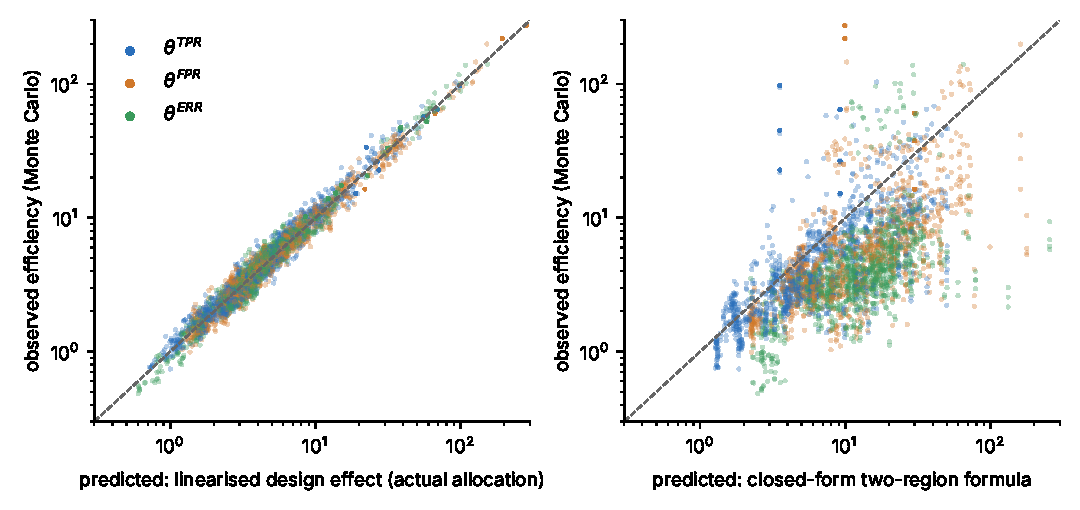
\includegraphics[width=\textwidth]{fig_sim_real}
\caption{Real pools, all budgets: observed efficiency of PATTERN relative to SRS for each of the
3519 compared target--budget pairs against the linearised prediction LIN (left) and the closed-form
two-region formula FORM (right). Dashed: equality. Source: \texttt{results/theory\_check.json}.}
\label{fig:sim-real}
\end{figure*}

\paragraph{The linearised design effect is accurate.} Over the 3519 pairs the ratio of observed to
predicted efficiency has median 0.998 and 10\%--90\% range 0.83--1.22; 77\% of the ratios are within
20\% and 99\% within a factor 1.5, and the correlation of the logarithms is 0.988
(Figure~\ref{fig:sim-real}, left). The spread is what Monte Carlo error alone produces: each MSE is
an average of 200 squared errors, with a relative standard error of about $\sqrt{2/200}=0.10$ for
approximately normal errors, so the ratio of two independent MSEs has a relative standard error of
about 0.14 and a 10\%--90\% range of roughly 0.84--1.20. The medians per pool and budget agree as
well: the ratio of the observed median efficiency to the median LIN prediction lies between 0.88 and
1.20 for the 34 pool--budget combinations, and for each type of estimand separately the median of
these ratios is 0.99 (TPR), 0.98 (FPR) and 1.00 (error). The agreement includes the cases with very
large gains: for Churn at $L=500$ the observed efficiency of 32.4 (predicted 32.2) arises because
the disagreement strata are fully enumerated, which only the finite-population corrections in LIN
capture. The lower correlations for Electricity, Phoneme and MAGIC reflect the narrow range of
efficiencies across targets in those pools (most lie between 2 and 4), not a larger error. We
conclude that, for the purpose of predicting efficiency, the linearised variance of
Section~\Mref{sec:theory-asym} is adequate already at $L=250$.

\paragraph{The closed form overstates the gain on real pools.} FORM is a much poorer predictor: the
median ratio of observed efficiency to FORM is 0.47 (10\%--90\%: 0.17--1.17), and the rule of thumb
$1/\rho$ is more optimistic still (Table~\ref{tab:sim-real}). The reason is the one anticipated in
Section~\Mref{sec:theory-deff}: with nine models the strata $(G,K)$ do not isolate the disagreements of
a particular pair. The share of the pool on which some model disagrees, $\rho_{\rm any}$, is between
0.18 and 0.73, while the median pairwise rate is between 0.001 and 0.33, and by
\eqref{eq:deff-sandwich} the attainable gain lies between $1/\rho_{\rm any}$ and $1/\rho$. OWN, which
uses the actual strata, is much closer (median ratio of observed to OWN 0.87): the remaining 13\% is
the price of serving all 108 estimands with one allocation, which Proposition~\Mref{prop:allocation}(d)
makes explicit. Law school is a degenerate case for FORM, since the median pair disagrees on 0.1\% of
the pool and many targets have nearly zero variance; FORM and the observed efficiencies are
negatively correlated there. FORM is therefore useful as an explanation of where the gain comes from
and as an upper guide for a pair-specific design, but not as a numerical prediction for the
nine-model design; for prediction, LIN should be used, and it requires nothing beyond the pool and a
pilot or proxy estimate of the stratum variances.

\subsection{Synthetic pools with a controlled disagreement rate}\label{sec:sim-synth}

To test the closed form where its assumptions hold, and to vary $\rho$ over a wide range, we
generated pools of $N=200\,000$ with two groups ($\zeta_1=0.3$, $p_0=0.30$, $p_1=0.20$). A share
$\rho\in\{1,2,5,10,20,40\}\%$ of instances is placed in a disagreement region. Outside it, all models
predict the same label, equal to $Y$ with probability 0.85. Inside it, with two models, model 1 is
right with probability $q_g$ and model 2 predicts the opposite label; we use $q=(0.65,0.35)$
(moderate group-wise gaps) and $q=(0.95,0.05)$ (large gaps, one-sided disagreements). With five
models, each model is right independently with a model- and group-specific probability between 0.40
and 0.70, conditionally on not all models agreeing. Each model's probability is
$\mathrm{logit}^{-1}\{1.73(2\hat y-1)+\varepsilon\}$ with $\varepsilon\sim N(0,1)$, and the proxy is their
average, as in the real pools. The budget is $L=1000$ and $R=1000$, so the Monte Carlo relative
standard error of an efficiency is about 0.06. With two models, the pattern strata separate agreement
from disagreement exactly, and we also ran, for each target, its own Neyman allocation computed from
the true stratum variances, which is the design FORM describes.

\begin{table*}[t]
\centering
\caption{Synthetic pools: observed (Obs), linearised (LIN) and closed-form (FORM) efficiency of
PATTERN relative to SRS for $\theta^{TPR}$ and $\theta^{ERR}$ (median over pairs for five models),
as a function of the disagreement rate $\rho$ ($N=200\,000$, $L=1000$, $R=1000$). Source:
\texttt{results/theory\_check.json}.}
\label{tab:sim-syn}
\setlength{\tabcolsep}{3pt}
\resizebox{\textwidth}{!}{%
\begin{tabular}{l rrr rrr @{\hskip 8pt} rrr rrr @{\hskip 8pt} rrr rrr}
\toprule
 & \multicolumn{6}{c}{Two models, moderate gaps} & \multicolumn{6}{c}{Two models, large gaps} & \multicolumn{6}{c}{Five models}\\
 \cmidrule(lr){2-7}\cmidrule(lr){8-13}\cmidrule(lr){14-19}
 & \multicolumn{3}{c}{$\theta^{TPR}$} & \multicolumn{3}{c}{$\theta^{ERR}$} & \multicolumn{3}{c}{$\theta^{TPR}$} & \multicolumn{3}{c}{$\theta^{ERR}$} & \multicolumn{3}{c}{$\theta^{TPR}$} & \multicolumn{3}{c}{$\theta^{ERR}$}\\
$\rho$ & Obs & LIN & FORM & Obs & LIN & FORM & Obs & LIN & FORM & Obs & LIN & FORM & Obs & LIN & FORM & Obs & LIN & FORM\\
\midrule
1\% & 190.3 & 216.0 & 102.2 & 174.1 & 181.1 & 115.5 & 56.2 & 55.8 & 46.2 & 665.4 & 608.0 & 517.0 & 172.9 & 198.3 & 170.7 & 158.1 & 162.9 & 203.2 \\
2\% & 54.3 & 57.4 & 43.7 & 56.7 & 58.2 & 55.7 & 22.2 & 26.0 & 23.4 & 251.5 & 240.7 & 261.2 & 44.9 & 64.2 & 82.9 & 49.8 & 55.3 & 99.7 \\
5\% & 14.9 & 18.6 & 16.6 & 23.2 & 20.2 & 22.1 & 10.0 & 9.7 & 9.5 & 88.1 & 83.1 & 103.7 & 17.4 & 21.0 & 32.9 & 19.5 & 19.6 & 40.1 \\
10\% & 7.2 & 8.9 & 8.4 & 8.6 & 9.6 & 10.9 & 4.4 & 5.1 & 5.1 & 45.6 & 42.5 & 53.5 & 9.2 & 11.0 & 17.5 & 8.9 & 9.4 & 20.1 \\
20\% & 4.4 & 4.7 & 4.6 & 5.0 & 4.8 & 5.5 & 2.4 & 2.8 & 2.8 & 16.7 & 20.3 & 25.6 & 4.9 & 5.4 & 9.0 & 4.7 & 4.6 & 10.0 \\
40\% & 2.3 & 2.5 & 2.5 & 2.4 & 2.4 & 2.7 & 1.7 & 1.6 & 1.8 & 9.5 & 10.1 & 12.4 & 2.5 & 2.8 & 4.7 & 2.3 & 2.3 & 5.0 \\
\bottomrule
\end{tabular}}
\end{table*}

\begin{figure*}[t]
\centering
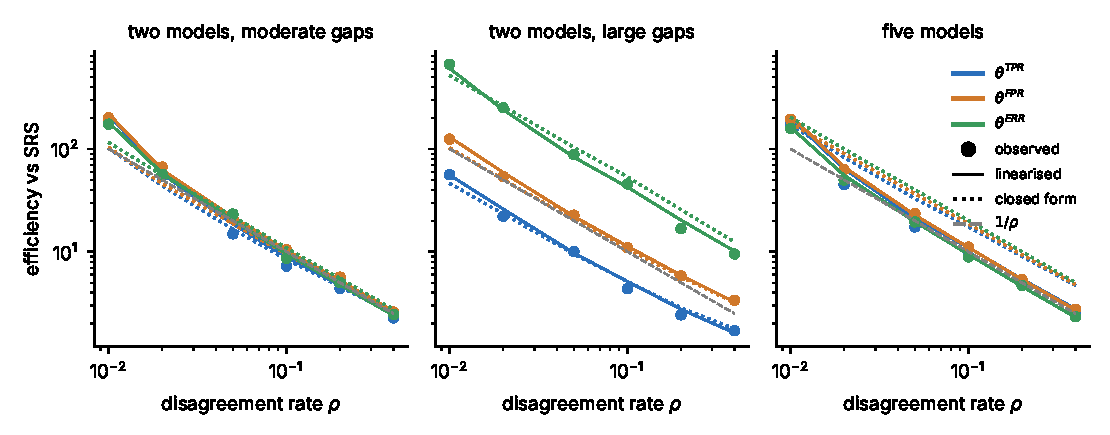
\includegraphics[width=\textwidth]{fig_sim_rho}
\caption{Synthetic pools: efficiency of PATTERN relative to SRS against the disagreement rate
$\rho$ (share of the pool in the disagreement region), median over pairs for each type of estimand.
Points: Monte Carlo ($R=1000$); solid: linearised prediction LIN; dotted: closed form FORM;
grey dashed: $1/\rho$. Source: \texttt{results/theory\_check.json}.}
\label{fig:sim-rho}
\end{figure*}

\paragraph{Efficiency scales as $1/\rho$.} In all three families the efficiency falls in proportion
to $1/\rho$ over a forty-fold range of $\rho$ (Figure~\ref{fig:sim-rho}). With two models and
moderate gaps, $\rho$ times the median observed efficiency (over all targets of the scenario, the three types of estimand pooled; Table~\ref{tab:sim-syn} shows them separately) is between 0.86 and 1.13 for
$\rho\ge2\%$, so the rule of thumb is accurate to about 15\%; at $\rho=1\%$ it is 1.9, because the
budget of 1000 labels is then about half the size of the disagreement region and the
finite-population correction roughly doubles the gain. LIN agrees with the observed efficiencies
throughout (median ratio per scenario between 0.88 and 1.04), with a tendency to be optimistic by a
few per cent that we attribute to the second-order terms neglected by the linearisation.

\paragraph{The closed form is accurate, and conservative, when its assumptions hold.} With two
models, the observed efficiency of the own-target Neyman design divided by FORM is between 0.90 and
1.25 for moderate gaps and $\rho\ge5\%$, and between 0.95 and 1.47 for large gaps; the LIN
predictions for the same designs give the same ratios, so the discrepancy is in the closed form and
not in the simulation. FORM is below the truth for two reasons stated in
Corollary~\ref{prop:deff}(a): it treats the agreement region as one stratum, whereas the pattern
design splits it by the common prediction ($K=0$ versus $K=M$, which have very different positive
rates), and it ignores the finite-population correction, which matters when the disagreement region
is small (at $\rho=1\%$ the ratio is 1.5 to 2.5). The large-gap family also shows the role of the
target size in Corollary~\ref{prop:deff}(c): the TPR gaps are large and the disagreements one-sided
($|a_g|=0.9$), and the gain for $\theta^{TPR}$ is only 0.45 to 0.7 times $1/\rho$, in line with
the factor $(\beta+\lambda)^{-2}$, which is about 0.4 for group 0 ($\pi_{\mathcal D}\approx
\pi_{\mathcal A}\approx0.3$) before the group factor $\Gamma$ is applied, while for the error difference, whose disagreements are nearly
deterministic within each group ($|\mu_g|=0.9$), the gain is several times $1/\rho$, as
\eqref{eq:deff-err} predicts.

\paragraph{With more models, the relevant rate is between $\rho_{\rm any}$ and the pairwise rate.} In
the five-model family the pairwise disagreement rate is about half of $\rho$, and FORM, which assumes
that each pair's disagreements are isolated, overstates the gain by a factor of about 1.9 (median
ratio of observed to FORM between 0.53 and 0.56 for $\rho\ge2\%$). The observed efficiency is instead
close to $1/\rho_{\rm any}$ ($\rho_{\rm any}$ times the median efficiency is between 0.94 and 1.06 for
$\rho\ge2\%$), the lower end of \eqref{eq:deff-sandwich}. This is expected: in this family the models
err independently inside the disagreement region, so a pair's disagreements are spread evenly over
the values of $K$. In the real pools, where models make correlated errors, the median OWN efficiency
lies inside the interval $[1/\rho_{\rm any},1/\rho]$ for every pool (Table~\ref{tab:sim-real}),
mostly in its lower half.

\subsection{Misspecified proxy}\label{sec:sim-proxy}

Proposition~\ref{prop:proxy} bounds the loss from a wrong proxy by the ratio \eqref{eq:proxy-loss}.
We took the five-model pool with $\rho=5\%$ and compared allocations computed from the default proxy,
from the true labels (oracle), from a constant proxy equal to the overall positive rate
(uninformative), from one minus the default proxy (inverted), and from an adversarial proxy that sets
$\pi_i=0.5$ where all models agree and $\pi_i=0.001$ where they do not, with proportional allocation
on the same strata as a reference.

\begin{table*}[t]
\centering
\caption{Proxy misspecification (five models, $\rho=5\%$, $L=1000$, $R=1000$). Loss: weighted
variance $\sum_tw_tV_t$ relative to the oracle allocation, predicted by the linearisation (pred.) and
observed with MSEs (obs.). Eff: harmonic mean over the 30 estimands of the efficiency relative to
SRS, predicted and observed, and the smallest observed efficiency. Kant.: Kantorovich bound of
Proposition~\ref{prop:proxy}(c) evaluated with the actual allocation. Source:
\texttt{results/theory\_check.json}.}
\label{tab:sim-proxy}
\small
\begin{tabular}{lrrrrrr}
\toprule
Allocation & Loss pred. & Loss obs. & Eff pred. & Eff obs. & min Eff obs. & Kant.\\
\midrule
Default proxy & 1.00 & 1.01 & 22.0 & 20.5 & 15.4 & 1.24\\
Oracle & 1.00 & 1.00 & 21.9 & 20.6 & 17.1 & 1.07\\
Uninformative & 1.00 & 1.01 & 21.9 & 20.5 & 16.6 & 1.23\\
Inverted & 1.00 & 0.98 & 22.0 & 21.2 & 17.2 & 1.24\\
Adversarial & 1.00 & 0.98 & 21.9 & 21.0 & 15.9 & 1.21\\
Proportional & 8.48 & 7.85 & 2.6 & 2.6 & 2.1 & 56.21\\
\bottomrule
\end{tabular}
\end{table*}

None of the four wrong proxies costs a measurable amount of efficiency (Table~\ref{tab:sim-proxy}):
the predicted loss is at most 0.2\%, the observed differences (between $-2.4\%$ and $+1.2\%$) are
within Monte Carlo error, and every one of the 30 estimands is estimated at least 15 times more
efficiently than under SRS. Proportional allocation on the same strata, by contrast, has eight times
the weighted variance. The explanation is Proposition~\Mref{prop:influence}: the proxy enters the
anticipated stratum variances only through label rates, while the dominant feature, namely that the
comparison estimands receive almost no variance from the strata where all models agree, is fixed by
the predictions. With a constant or adversarial proxy the agreement strata are still anticipated to
have variance of order $\delta_g^2$, which is small, and the disagreement strata still have variance
of order one because $D_i$ varies within them; so all these allocations put almost the whole budget
into the disagreement strata and differ only in how it is divided among them. The Kantorovich bounds
(1.21--1.24) are valid but loose here. This robustness is specific to the structure of the problem
and should not be read as a general guarantee: Proposition~\ref{prop:proxy}(d) shows that a proxy
that misjudges a high-variance stratum can do arbitrarily badly in other stratified problems, and the
empirical comparison with the oracle allocation in Section~\Mref{sec:ablations} is the relevant check
for real data.

\subsection{The difference estimator (PATTERN-DIF)}\label{sec:sim-dif}

Section~\Mref{sec:theory-dif} makes four predictions about the difference estimator (\Mref{eq:dif}) with the proxy mean (\Mref{eq:psi}): it is exactly unbiased for the totals
for any proxy and its plug-in variance is unbiased (Proposition~\Mref{prop:validity}); its linearised variance is $V_\psi=\sum_hc_hS^2_{e,h}$ with residual influence values
$e_i=z_i-\tilde z_i$; its gain over the plain estimator on the same sample is $V_0/V_\psi$, which a label-free calculation forecasts under calibration
(Proposition~\Mref{prop:dif-deff}); and a miscalibrated proxy can lose to the plain estimator (Proposition~\ref{prop:dif-proxy}). We check them with
\texttt{experiments/theory\_check\_dif.py} (results in \texttt{results/theory\_check\_dif.json}). Every comparison is between the plain and the
difference estimator on the \emph{same} PATTERN sample, so the ratio $\mathrm{MSE}(\text{plain})/\mathrm{MSE}(\text{DIF})$ isolates the estimator. Three predictions are used:
\textbf{LIN}, $\sum_hc_hS^2_{z,h}/\sum_hc_hS^2_{e,h}$, computed with the true labels; \textbf{ANT}, the label-free forecast
$\sum_hc_h(\bar\sigma^2_h+S^2_{\tilde z,h})/\sum_hc_h\bar\sigma^2_h$ of (\Mref{eq:dif-deff}), which uses the proxy only; and \textbf{TUNE}, $V_\psi/V(\lambda)$ with $\lambda_h=\min\{1,\max(0,\beta_h)\}$, the
most that tuning the coefficient could add to $\lambda=1$.

\paragraph{Exactness and the variance formulae.} On a pool of 14 units in two strata (6 and 8 units, 2 and 3 labels) we enumerated all 840 samples for three proxies (a random mixture of $u_i,v_i$, an arbitrary bounded vector, and
the anti-correlated vector $1-t_i$) and three coefficients ($\lambda=0,\frac12,1$). The mean of $\hat T_{\lambda\psi}$, its covariance matrix and the mean of the plug-in variance estimator agree with $T$,
the formula of Proposition~\Mref{prop:validity}(a) and each other to within $3\times10^{-13}$ in absolute terms (relative to the variances, $10^{-14}$), that is machine precision, for every proxy. By Monte Carlo ($R=2000$) the totals are also unbiased on the four real pools and six synthetic pools: the largest standardised bias
over the 29--49 coordinates is $|z|=2.7$ for the difference estimator and 2.6 for the plain estimator, which share their samples and have strongly correlated coordinates, and the largest bias is 0.06 standard deviations
(the Monte Carlo resolution is 0.022). The variance formula holds: the median over estimands of the Monte Carlo variance divided by the linearised $V_\psi$ is between 0.99 and 1.02 on the real pools (Table~\ref{tab:sim-dif-real}) and 1.01 to 1.07 on the synthetic
pools (up to 1.10 for $\theta^{TPR}$, a second-order effect of the random denominators at $L=600$), the mean of $\hat V_\psi$ divided by the Monte Carlo variance is between 0.98 and 1.02, and the Wald coverage of the difference estimator
(0.943 to 0.951 on the real pools, 0.947 to 0.953 on the synthetic pools) is that of the plain estimator.

\begin{table*}[t]
\centering
\caption{Four real pools, $R=2000$: efficiency of the difference estimator relative to the plain estimator on the same PATTERN sample (median over the 108 estimands). Obs: Monte Carlo; LIN, ANT, TUNE:
predictions defined in the text; Obs/LIN: per-target ratio, median and 10\%--90\% range, and correlation of the logarithms; Var: Monte Carlo variance of $\hat\theta_{\rm DIF}$ over $V_\psi$; $\hat V$: mean estimated over Monte Carlo variance; Cov: Wald coverage of plain
and difference estimator; max $|z|$: largest standardised bias of the 46--49 totals. Source: \texttt{results/theory\_check\_dif.json}.}
\label{tab:sim-dif-real}
\small
\resizebox{\textwidth}{!}{%
\begin{tabular}{lrrrrrlrrrrrr}
\toprule
Pool & $L$ & Obs & LIN & ANT & TUNE & Obs/LIN & corr & Var & $\hat V$ & Cov plain & Cov DIF & max $|z|$\\
\midrule
Adult-sex & 500 & 1.50 & 1.46 & 1.47 & 1.01 & 1.01 (0.99, 1.04) & 0.998 & 0.99 & 1.02 & 0.949 & 0.951 & 1.6\\
Bank & 500 & 1.45 & 1.48 & 1.46 & 1.01 & 0.99 (0.96, 1.03) & 0.994 & 1.02 & 0.99 & 0.942 & 0.943 & 2.0\\
EEG & 500 & 1.90 & 1.91 & 1.43 & 1.04 & 1.00 (0.97, 1.03) & 0.997 & 1.00 & 1.00 & 0.947 & 0.948 & 2.2\\
Spambase & 250 & 2.30 & 2.34 & 1.97 & 1.02 & 1.00 (0.96, 1.03) & 0.998 & 1.00 & 0.99 & 0.944 & 0.945 & 1.4\\
\bottomrule
\end{tabular}}
\end{table*}

\begin{figure*}[t]
\centering
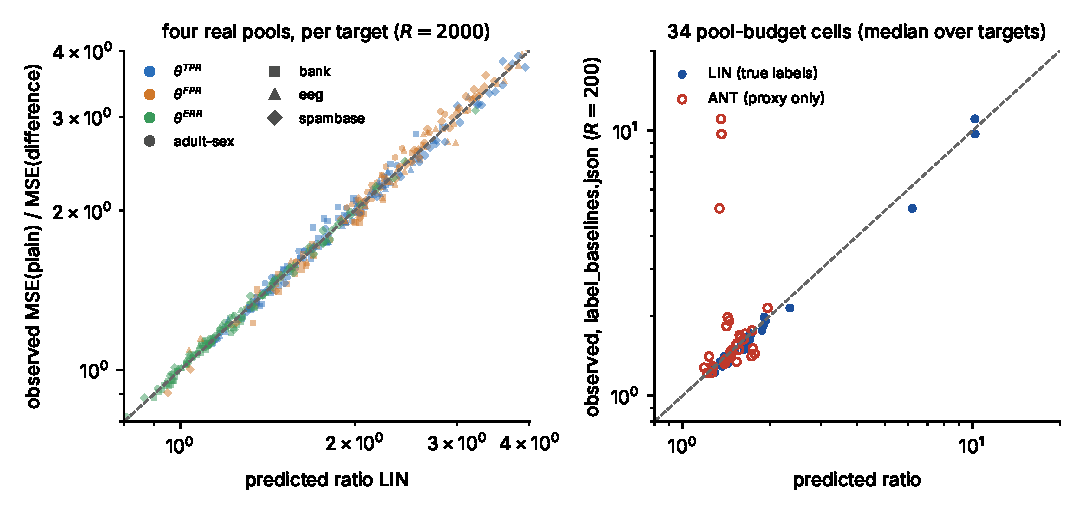
\includegraphics[width=\textwidth]{fig_sim_dif_real}
\caption{Left: observed against linearised (LIN) gain of the difference estimator over the plain estimator, per estimand, on four real pools ($R=2000$; 432 estimands). Right: median over estimands in each of 34 pool--budget
cells, observed in \texttt{results/label\_baselines.json} (PATTERN-DIF against PATTERN, $R=200$) against LIN (filled) and ANT (open). Dashed: equality. Source: \texttt{results/theory\_check\_dif.json}.}
\label{fig:sim-dif-real}
\end{figure*}

\paragraph{Predicted against observed gain.} On the four real pools the observed per-estimand gain divided by LIN has median 1.00 and 10\%--90\% range 0.97--1.04 (432 estimands, correlation of the logarithms 0.997; Figure~\ref{fig:sim-dif-real}, left), which
is Monte Carlo error. We then compared LIN with the gains stored in \texttt{results/label\_baselines.json}, which were produced independently by \texttt{experiments/label\_baselines.py} with $R=200$. In the 34 cells with a defined gain (all 35 except Law school at
$L=2000$, where both estimators are exact) the observed median gain is 1.47 (10\%--90\% range 1.28--2.10, extremes 1.22 and 11.1), LIN has median 1.49, and the ratio of observed to LIN has median 0.98 (10\%--90\% range 0.93--1.01, 97\% of cells within 20\%, correlation of the logarithms 0.996, 0.978 without
the three Law school cells); Figure~\ref{fig:sim-dif-real} (right). LIN uses the labels, so it is not a forecast, but it confirms that the residual-variance formula $V_\psi$ describes the estimator. The label-free forecast
ANT has median ratio 1.01 (0.90--1.37) over cells, and on the four real pools ratio 1.12 (0.86--1.53) with correlation 0.78 across estimands; the observed gain is 1.30 and 1.37 times ANT in EEG and Spambase. It fails in Law school (forecast 1.3--1.4, observed 5.1--11.1), where the
disagreement sets of most pairs contain a handful of units per stratum: the realised residual variance is then a single draw from the label distribution, and it is an order of magnitude below its expectation under the proxy (we checked the stratum variances for one estimand). Without Law school the correlation of ANT with the observed gain is 0.62.
The gain is therefore not a doubling in general: it is 1.2 to 1.7 in most cells, about 1.8 to 2.1 in EEG and Spambase, and 5 to 11 only in Law school. By estimand type the order is that of \eqref{eq:dif-closed}: the gain is largest for $\theta^{FPR}$,
next for $\theta^{TPR}$ and smallest for $\theta^{ERR}$ (Adult-sex: 2.25, 1.67 and 1.13; Table~\ref{tab:sim-dif-syn} for the synthetic pools).

\paragraph{Tuning the coefficient.} TUNE is small: the median over the 34 cells is 1.02 (10\%--90\% 1.01--1.04), and 1.01 to 1.04 on the four real pools, so a perfectly tuned coefficient would add at most a few per cent to $\lambda=1$ except in Law school (2.3--3.5).
The observed estimated-coefficient version (PATTERN-PPI) has median gain 1.03 over $\lambda=1$ (10\%--90\% 0.99--1.10), and it costs coverage: mean coverage over the 35 cells is 0.946 for PATTERN-DIF and 0.929 for PATTERN-PPI, and 8 of 35 cells fall below 0.93 for PATTERN-PPI against 1 of 35 for PATTERN-DIF
and for the plain estimator. This is the trade-off of Proposition~\ref{prop:dif-lambda}.

\paragraph{Allocation.} The residual-variance allocation of Proposition~\ref{prop:alloc-dif} does not improve on the design's plain-variance allocation for the difference estimator. The linearised prediction of the ratio of $V_\psi$ under the plain allocation to $V_\psi$ under the residual allocation has median 0.99
(10\%--90\% 0.95--1.00) over the 34 cells, and on four real pools the observed ratio of mean squared errors is 0.98, 0.98, 0.98 and 1.01, against linearised predictions 1.00, 1.00, 0.98 and 1.00, with the same coverage. Using the ``wrong'' variances therefore costs at most about 2\% here, as the bound \eqref{eq:alloc-loss} allows when the signal-to-noise ratio $\tilde\nu_h$ is similar across strata.

\begin{table*}[t]
\centering
\caption{Synthetic pools ($N=60\,000$, five models, $Y_i\sim$ Bernoulli$(\pi_i)$, $L=600$, $R=2000$): gain of the difference estimator over the plain estimator, observed (Obs), linearised (LIN) and label-free (ANT), median over the ten pairs. Top: calibrated proxy,
sharpness $a$ of the latent score. Bottom: $a=2$, proxy $\pi^{\rm proxy}_i=\mathrm{logit}^{-1}(\kappa s_i)$ ($\kappa=1$ calibrated, $\kappa=0$ constant 0.5, $\kappa<0$ inverted). Source: \texttt{results/theory\_check\_dif.json}.}
\label{tab:sim-dif-syn}
\setlength{\tabcolsep}{4pt}
\small
\begin{tabular}{l rrr rrr rrr}
\toprule
 & \multicolumn{3}{c}{$\theta^{TPR}$} & \multicolumn{3}{c}{$\theta^{FPR}$} & \multicolumn{3}{c}{$\theta^{ERR}$}\\
 \cmidrule(lr){2-4}\cmidrule(lr){5-7}\cmidrule(lr){8-10}
 & Obs & LIN & ANT & Obs & LIN & ANT & Obs & LIN & ANT\\
\midrule
$a=0.5$ & 1.76 & 1.76 & 1.76 & 2.40 & 2.44 & 2.47 & 1.10 & 1.09 & 1.10 \\
$a=1$ & 2.03 & 1.97 & 1.98 & 2.33 & 2.33 & 2.36 & 1.09 & 1.09 & 1.10 \\
$a=2$ & 2.11 & 2.12 & 2.14 & 2.21 & 2.32 & 2.31 & 1.11 & 1.12 & 1.11 \\
$a=4$ & 2.23 & 2.23 & 2.24 & 2.26 & 2.27 & 2.26 & 1.11 & 1.12 & 1.12 \\
\midrule
$\kappa=-1$ & 1.43 & 1.48 & 2.29 & 1.52 & 1.56 & 2.15 & 0.76 & 0.76 & 1.12 \\
$\kappa=0$ & 1.88 & 1.94 & 2.00 & 2.04 & 2.05 & 2.00 & 1.00 & 1.00 & 1.00 \\
$\kappa=0.5$ & 2.11 & 2.11 & 2.02 & 2.23 & 2.22 & 2.09 & 1.10 & 1.09 & 1.03 \\
$\kappa=1$ & 2.21 & 2.16 & 2.15 & 2.28 & 2.27 & 2.29 & 1.12 & 1.12 & 1.12 \\
$\kappa=2$ & 2.09 & 2.06 & 2.59 & 2.22 & 2.17 & 2.89 & 1.08 & 1.07 & 1.39 \\
$\kappa=4$ & 1.81 & 1.80 & 3.81 & 1.89 & 1.90 & 4.45 & 0.96 & 0.94 & 2.11 \\
\bottomrule
\end{tabular}
\end{table*}

\begin{figure*}[t]
\centering
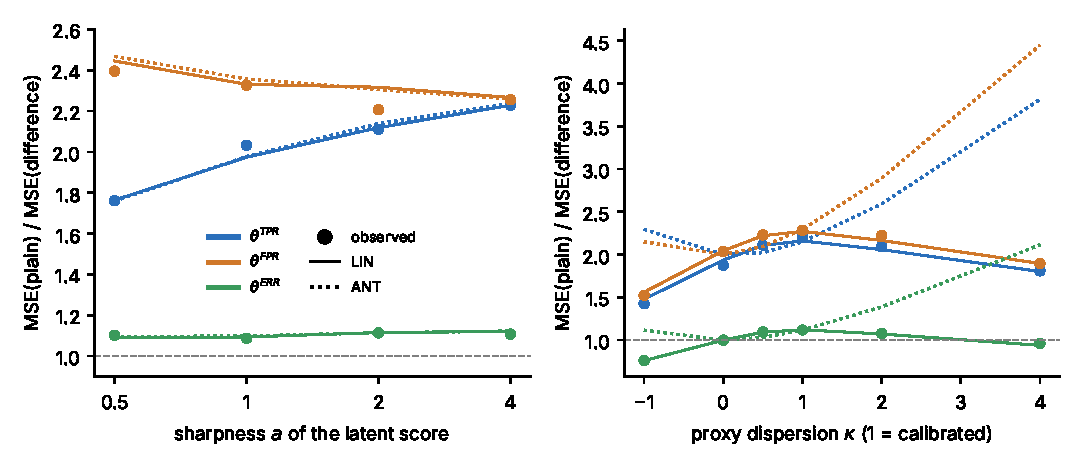
\includegraphics[width=\textwidth]{fig_sim_dif_synth}
\caption{Synthetic pools, gain of the difference estimator over the plain estimator (median over pairs, by estimand). Left: calibrated proxy, sharpness $a$ of the latent score. Right: $a=2$, proxy dispersion $\kappa$ ($\kappa=1$ calibrated).
Points: Monte Carlo ($R=2000$); solid: LIN; dotted: ANT, which assumes calibration. Dashed: no gain. Source: \texttt{results/theory\_check\_dif.json}.}
\label{fig:sim-dif-synth}
\end{figure*}

\paragraph{Calibrated and miscalibrated proxies.} In pools whose labels follow the proxy, ANT and LIN agree with each other and with the Monte Carlo gain within 2\% (median observed/LIN between 0.99 and 1.00; Table~\ref{tab:sim-dif-syn}, top), which verifies
Proposition~\Mref{prop:dif-deff}: the gain is 1.8 to 2.4 for the rate differences and 1.1 for the error difference, because in the disagreement strata the proxy is uncertain ($\overline{\pi(1-\pi)}$ is large) and the closed forms \eqref{eq:dif-closed} are bounded; a sharper latent score hardly changes them. For miscalibrated proxies
(bottom), unbiasedness and coverage are unaffected (coverage 0.947--0.953), LIN keeps tracking the Monte Carlo gain (median ratio 0.99 to 1.01) and ANT, which assumes calibration, does not. The theory's two warnings appear. First, an inverted proxy ($\kappa=-1$) makes the difference estimator \emph{worse} than the plain estimator for the error difference
(gain 0.76, that is 1.3 times the mean squared error, as LIN predicts), while the rate differences still gain 1.4 to 1.5. The design-weighted slope $\bar\beta=\sum_hc_h\mathrm{Cov}_h(z,\tilde z)/\sum_hc_hS^2_{\tilde z,h}$ of the error difference is $-1.02$, the clipped coefficient is $0$ and TUNE, which here recovers the plain estimator, is 1.32 $=1/0.76$. Second, a constant proxy $\pi_i\equiv\frac12$ ($\kappa=0$) is uninformative for the error difference (gain exactly 1, since $\tilde z\equiv0$) but not for the
rate differences (1.9 and 2.0, TUNE 1.03 and 1.04), because $\tilde z_i$ still carries the known pattern of $D_i$. Third, the threshold $\beta<\frac12$ of Proposition~\Mref{prop:dif-var}(a) is visible: for the error difference $\bar\beta$ is 1.02 at $\kappa=1$, 0.62 at $\kappa=2$ (gain 1.08) and 0.44 at $\kappa=4$ (gain 0.96), so an over-sharp proxy gains little for the rate differences (1.8--1.9) and crosses to a loss for the error difference.

\paragraph{Zero-variance strata and the floor.} The residual floor \eqref{eq:floor} was evaluated on four pools at $L=250$ ($R=1000$). At Churn the difference estimator alone raises the worst-estimand coverage from 0.52 (plain estimator, \texttt{results/label\_baselines.json}) to 0.84 (0.87 in this run), because
$\hat e_i=-\pi_i\hat d_i$ varies even when no positive is sampled; at Law school it does not (0.64 for both). Where the problem persists the floor repairs it: for Law school mean coverage rises from 0.913 to 0.954 and the worst-estimand coverage from 0.65 to 0.89; for Adult-sex and Credit card default the mean rises from 0.942 to 0.946 and from 0.949 to 0.955 with the worst estimand unchanged (0.85 and 0.92); at Churn the floor is active in 0.2\% of
(replication, estimand) pairs and changes nothing (0.938). The floor widens the intervals by a median factor of 1.00 (90th percentile 1.08, 1.15, 1.33 for Adult-sex, Credit card and Law school). It does not alter the point estimate. As in Section~\Mref{sec:ablations} it is a safeguard chosen after seeing the failure, and these numbers are not an out-of-sample test.

\subsection{Summary}

The linearised design effect predicts the efficiency of the implemented design to within Monte
Carlo error on all 11 real pools and in the synthetic families (per-target median ratio 1.00,
10\%--90\% range 0.83--1.22 on the real pools). The closed form of Corollary~\ref{prop:deff} is
accurate and conservative when the strata separate a pair's agreements from its disagreements (the
own-target efficiency is 0.90 to 1.47 times the formula for $\rho\ge5\%$), and it captures the $1/\rho$ scaling and the effect of the
target size. With nine models it overstates the gain on real pools by a median factor of about two,
because the counts $K$ locate any disagreement but not that of a specific pair; the bounds
$1/\rho_{\rm any}\le\mathrm{Eff}\le1/\rho$ of \eqref{eq:deff-sandwich} describe this gap. The gain vanishes
only as the disagreement rate approaches one, as in EEG ($\rho_{\rm any}=0.73$, efficiency 1.6--1.9). For the difference estimator the linearised residual variance predicts the observed gain over the plain estimator within Monte Carlo error
(median ratio 0.98 over 34 pool--budget cells; Section~\ref{sec:sim-dif}), the label-free forecast does so except in Law school, and the gain is moderate (median 1.47) rather than a doubling.

\section{Baseline designs and detailed results}\label{si:baselines}

This section gives the full definitions of the baselines compared in Section~\Mref{sec:baselines}, the per-setting results and the detailed coverage discussion.

\paragraph{Common ground.} To make the comparison about the choice of labels and estimators and nothing else, every method estimates the same vector of totals $T$ (Section~\Mref{sec:setting}), plugs it into the same map $\hat\theta=f(\hat T)$ for all $3\binom{M}{2}=108$ comparison estimands $\theta^{\mathrm{TPR}}_{mj},\theta^{\mathrm{FPR}}_{mj},\theta^{\mathrm{ERR}}_{mj}$, and reports 95\% Wald intervals from a linearisation variance. Every method that uses a proxy uses the same $\pi_i=M^{-1}\sum_m\hat p_{mi}$, and every allocation over several estimands uses the same weights $w_k=1/S_k^2$ as (\Mref{eq:alloc}). The budget is counted in distinct labelled instances. Pool labels are used only to answer label queries, to compute the truth and, for reporting, to pick the three most accurate models. Estimands whose numerator is identically zero in the pool (the two models never disagree on the relevant instances) are estimated exactly by every design and are left out of all summaries. This removes 51 of the 108 estimands in the law-school setting, including all those among its three most accurate models, and none elsewhere.

\subsection{Baseline definitions}


\paragraph{B1: importance sampling for active comparison.} \citet{sawade2012active} compare the risks of two fixed models by drawing $n$ instances with replacement from an instrumental distribution $q$ and estimating each risk by the self-normalised weighted mean $\sum_k \ell_k/q_k\big/\sum_k 1/q_k$ (with $p(x)=1/N$ on a pool). Their Theorem~1 shows that the asymptotic variance of the estimated risk difference is minimised by $q^*(x)\propto p(x)\{\mathbb E[(\ell_1-\ell_2-\Delta)^2\mid x]\}^{1/2}$. They replace $p(y\mid x)$ by an equal mixture of the models' predictive distributions, and for $k$ models they use the equal mixture of the pairwise-optimal distributions. We keep all of this and change only the quantity being compared. With replacement draws $i_1,\dots,i_n\sim q$, our totals are the Hájek (self-normalised) estimators
\begin{align*}
\hat T^{\mathrm{IS}}&=N\,\frac{\sum_{k=1}^n t_{i_k}(Y_{i_k})/q_{i_k}}{\sum_{k=1}^n 1/q_{i_k}},\\
\hat\theta-\theta&\approx\frac1n\sum_{k=1}^n \frac{a_{i_k}}{q_{i_k}},\\
a_i&=\nabla f(T)^{\top}\{t_i(Y_i)-T/N\}.
\end{align*}
For $\theta^{\mathrm{ERR}}_{mj}$, $a_i=\{|\hat y_{mi}-Y_i|-|\hat y_{ji}-Y_i|-\theta^{\mathrm{ERR}}_{mj}\}/N$, which is exactly Sawade et al.'s centred loss difference. For $\theta^{\mathrm{TPR}}_{mj}$, the self-normalisation is automatic because $f$ is a ratio, and $a_i=\sum_g s_g\,\mathbf 1\{G_i=g\}\,Y_i\{(\hat y_{mi}-\hat y_{ji})-(\mathrm{TPR}_{mg}-\mathrm{TPR}_{jg})\}/P_g$. The asymptotic variance is $n^{-1}\sum_i\mathbb E[a_i^2]/q_i$ \citep{hansen1943}, so the single-estimand optimum is $q_i\propto\{\mathbb E_\pi a_i^2\}^{1/2}$, with the expectation taken under $Y_i\sim\mathrm{Bernoulli}(\pi_i)$ and $a$ evaluated at the proxy totals. This is our adaptation to TPR and FPR gaps. For a pair $(m,j)$ we combine its three estimands as $q^{(mj)}_i\propto\{\sum_{k\in(m,j)}w_k\mathbb E_\pi a_{ik}^2\}^{1/2}$. The design distribution is the equal mixture over the 36 pairs, as in Sawade et al., mixed with the uniform distribution with weight $0.05$ so that every $q_i$ is bounded away from zero. Draws continue until $L$ distinct instances are labelled; repeated draws reuse the label. The median number of draws was $1.12L$ (range $1.02L$--$1.48L$), so B1 effectively gets more than $L$ draws for $L$ labels. The variance is estimated by $n^{-1}$ times the sample variance of $\hat a_{i_k}/q_{i_k}$.

\paragraph{B2: proxy-score stratification.} The classic approach to estimating a classifier's metrics with few labels stratifies on the classifier's score and allocates optimally \citep{bennett2010online,kumar2018classifier}. We form strata as group $\times$ within-group quantile bins of $\pi_i$ (10 bins, Score-10; and 5 bins, Score-5), merge strata smaller than 50 as for PATTERN, and use the same estimator (\Mref{eq:HT}), variance (\Mref{eq:var}) and proxy-Neyman allocation (\Mref{eq:alloc}). B2 therefore differs from PATTERN only in the strata. It uses the proxy strongly but ignores which models disagree.

\paragraph{B3: disagreement-focused two-phase design.} Labelling only where models disagree is the ``active $\neq$'' baseline of \citet{sawade2012active} and the discordant-pair approach of \citet{musgrove2023discordant} and of the screening-test literature \citep{pepe2001comparing}. On its own it identifies only ratios, because the denominators $P_g,Q_g$ need labels in the agreement set. Let $D=\{i:0<K_i<M\}$ and $A=U\setminus D$. Phase 1 draws a simple random sample $s_0$ of size $n_0$ from $U$. Phase 2 draws a simple random sample of $L-n_0$ from $D\setminus s_0$. Conditionally on $n_A=|s_0\cap A|$, the labelled units in $A$ are a simple random sample from $A$. Conditionally on $|s_0\cap D|$, the union of $s_0\cap D$ and the phase-2 sample is a simple random sample of size $n_D=|s_0\cap D|+L-n_0$ from $D$. The combined estimator is therefore the two-stratum estimator $\hat T=N_A\bar t_A+N_D\bar t_D$ with variance (\Mref{eq:var}) at the realised $(n_A,n_D)$, which is conditionally design-unbiased. We take $n_0=L/4$ (Dis-25) and $n_0=L/2$ (Dis-50).

\paragraph{B4: prediction-powered inference.} PPI \citep{angelopoulos2023ppi} corrects the predictions on the whole pool with the labelled residuals. With the prediction of $t_i$ taken as its proxy mean $\tilde t_i=\pi_iu_i+(1-\pi_i)v_i$, the PPI estimator of a total under SRS is the difference estimator
\[
\hat T^{\mathrm{PPI}}_\lambda=\lambda\sum_{i\in U}\tilde t_i+\frac Nn\sum_{i\in s}\{t_i(Y_i)-\lambda\tilde t_i\},
\]
with $\lambda=1$ (PPI). PPI++ \citep{angelopoulos2026ppipp} tunes $\lambda$ for each estimand. In our finite-pool setting the predictions are known for every unit, so the $(1+n/N)$ factor of PPI++ drops out and the variance-minimising value is the regression coefficient of $\nabla f^\top t_i$ on $\nabla f^\top\tilde t_i$ in the sample. We clip it to $[0,1]$. StratPPI \citep{fisch2024stratppi} applies PPI++ within strata with a stratum-specific $\lambda_{hk}$ and allocates the budget by a Neyman rule on the residual standard deviation, estimated from the predictor's own confidence scores. We use the B2 strata (group $\times$ 10 proxy bins), per-stratum and per-estimand $\lambda_{hk}$ clipped to $[0,1]$, and the allocation $n_h\propto N_h\{\sum_k w_k\,\overline{\pi(1-\pi)(A_{k}-B_{k})^2}_h\}^{1/2}$. Here $\pi_i(1-\pi_i)(A_{ik}-B_{ik})^2$ is the proxy variance of the residual $z_{ik}-\mathbb E_\pi z_{ik}$, so this allocation is Fisch et al.'s confidence-based rule for our estimands. In all three versions the variance is the stratified formula (\Mref{eq:var}) applied to the residuals $z_{ik}-\lambda\,\nabla f^\top\tilde t_i$.

\paragraph{B5: PATTERN with a model-assisted estimator (the proposed method).} The PPI correction is a difference or GREG-type estimator \citep[Chapter~6]{sarndal1992} and can be applied to the PATTERN sample without changing the design. PATTERN-DIF uses the stratified difference estimator with $\lambda=1$. PATTERN-PPI tunes $\lambda_{hk}$ per stratum as in StratPPI. B5 is the proposed method (PATTERN-DIF, $\lambda=1$) and a tuned-weight variant (PATTERN-PPI), and is reported in the last block of the results.

\paragraph{Not run.} Active testing with LURE \citep{kossen2021active}, adaptive variance-minimising selection \citep{hara2024}, and active inference \citep{zrnic2024active,li2025robust} select labels sequentially and target one estimand of one model. Their fixed-budget, one-shot analogue for our vector of estimands is B1, which uses the same proxy-optimal inclusion principle. Model-based estimators that need a fitted joint model of labels and scores (for example SSME) are outside the design-based comparison made here.

\subsection{Detailed results}

\begin{figure*}[t]\centering
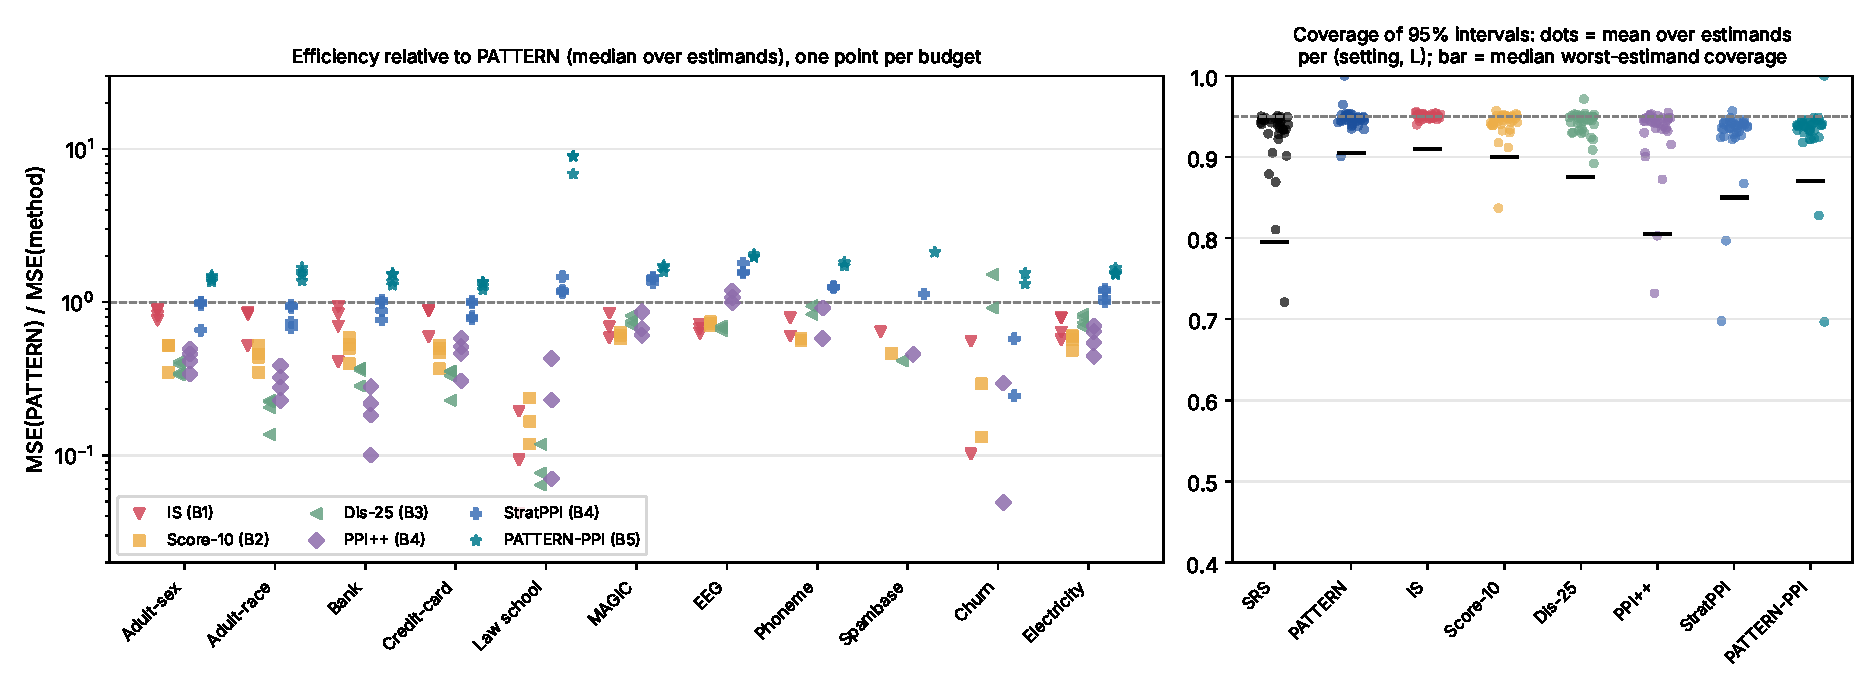
\includegraphics[width=\textwidth]{base_efficiency}
\caption{Left: MSE(PATTERN)/MSE(method) by setting, one point per budget, median over comparison estimands (values above 1 mean that the method beats PATTERN; the axis is clipped to $[0.02,30]$ and law school at $L=2000$ is not shown in range because PATTERN labels the whole disagreement set there). Right: mean coverage of the nominal 95\% interval over estimands for each (setting, $L$), with the median over cells of the worst-estimand coverage as a bar. Source: \texttt{results/label\_baselines.json}.}\label{fig:base-efficiency}
\end{figure*}

\begin{table*}[t]\centering\footnotesize
\caption{Efficiency relative to PATTERN, MSE(PATTERN)/MSE(method), median over estimands, by setting at $L=500$ ($L=250$ for Spambase, whose pool is too small for $L=500$). Values above 1 mean that the method beats PATTERN. Second column: efficiency of PATTERN relative to SRS. Last two columns: mean coverage of the 95\% intervals of StratPPI and of PATTERN-PPI. Source: \texttt{results/label\_baselines.json}.}\label{tab:base-setting}
\setlength{\tabcolsep}{3.5pt}
\resizebox{\textwidth}{!}{\begin{tabular}{l rrrrrrrrrrr}\toprule
 & PAT. & \multicolumn{6}{c}{Baselines (B1--B4) vs PATTERN} & \multicolumn{2}{c}{B5 vs PATTERN} & \multicolumn{2}{c}{Coverage} \\
\cmidrule(lr){3-8}\cmidrule(lr){9-10}\cmidrule(lr){11-12}
Setting & vs SRS & IS & Score-10 & Dis-25 & Dis-50 & PPI++ & StratPPI & PATTERN-DIF & PATTERN-PPI & StratPPI & PAT-PPI \\ \midrule
Adult-sex & 4.19 & 0.89 & 0.52 & 0.39 & 0.37 & 0.46 & 0.97 & 1.45 & 1.49 & 0.935 & 0.939 \\
Adult-race & 7.27 & 0.86 & 0.46 & 0.23 & 0.22 & 0.32 & 0.93 & 1.44 & 1.58 & 0.939 & 0.939 \\
Bank & 8.26 & 0.84 & 0.50 & 0.36 & 0.38 & 0.22 & \textbf{1.03} & 1.47 & 1.52 & 0.941 & 0.933 \\
Credit-card & 3.71 & 0.89 & 0.52 & 0.36 & 0.35 & 0.51 & \textbf{1.01} & 1.28 & 1.35 & 0.937 & 0.933 \\
Law school & 39.0 & 0.09 & 0.24 & 0.08 & 0.08 & 0.23 & \textbf{1.47} & 11.1 & 8.97 & 0.797 & 0.828 \\
MAGIC & 2.93 & 0.69 & 0.63 & 0.75 & 0.63 & 0.67 & \textbf{1.43} & 1.70 & 1.73 & 0.942 & 0.943 \\
EEG & 1.70 & 0.67 & 0.73 & 0.70 & 0.66 & \textbf{1.19} & \textbf{1.57} & 1.98 & 2.05 & 0.926 & 0.939 \\
Phoneme & 3.53 & 0.60 & 0.58 & 0.83 & 0.67 & 0.58 & \textbf{1.26} & 1.71 & 1.72 & 0.946 & 0.941 \\
Spambase$^{\ast}$ & 5.77 & 0.64 & 0.46 & 0.42 & 0.37 & 0.46 & \textbf{1.13} & 2.14 & 2.12 & 0.925 & 0.933 \\
Churn & 34.6 & 0.10 & 0.13 & \textbf{1.52} & 0.28 & 0.05 & 0.24 & 1.28 & 1.32 & 0.930 & 0.932 \\
Electricity & 2.86 & 0.79 & 0.59 & 0.80 & 0.73 & 0.64 & \textbf{1.21} & 1.49 & 1.53 & 0.942 & 0.933 \\
\bottomrule\end{tabular}}\end{table*}


\paragraph{Where a baseline beats PATTERN.} Table~\ref{tab:base-setting} and Figure~\ref{fig:base-efficiency} show where the ranking changes. First, StratPPI beats PATTERN at $L=500$ in seven of the ten settings of the table (ratios 1.01--1.57 in Bank, Credit-card, Law school, MAGIC, EEG, Phoneme and Electricity, and 1.13 in Spambase at $L=250$), and is below it in Adult-sex (0.97), Adult-race (0.93) and Churn (0.24). Over all cells its ratio exceeds 1 in 19 of 35 (median 1.12 at $L=500$). The margin is small in most settings, and it is not a failure of the stratification: StratPPI uses the same sample size but a model-assisted estimator, and B5 shows that the same correction applied to the PATTERN sample improves PATTERN itself by a median factor of 1.3--1.7. Second, Dis-25 beats PATTERN on Churn at $L=500$ (ratio 1.52); there the pool has a 19\% disagreement set, PATTERN strata are mostly small, and Dis-25 labels most of its sample inside the disagreement set. Its intervals are not reliable in that cell: mean coverage 0.93 but worst-estimand coverage 0.66, so the apparent gain should be read with caution. Third, PPI++ beats PATTERN on EEG (ratio 1.19 at $L=500$), the setting with the largest disagreement set (73\%), where agreement cells hold little and the proxy is informative. Importance sampling never beats PATTERN in the all-estimand median (ratio below 1 in all 35 cells), but on the pairs among the three most accurate models it is competitive: its median efficiency against SRS on those pairs is 4.2, 4.1, 4.2 and 6.3 at $L=250,\dots,2000$, against 3.4, 3.6, 4.0 and 6.8 for PATTERN, and it beats PATTERN on those pairs in 10 of 35 cells (Adult-sex: 1.49 at $L=250$ and 1.10 at $L=500$, while its all-estimand ratio there is 0.89). Where the question is only about the best few models, importance sampling is a serious alternative.

\paragraph{Where PATTERN wins clearly.} In the two settings with the lowest disagreement rate, Law school and Churn, PATTERN is 6--84 times more efficient than SRS at $L\le1000$ and PATTERN labels essentially every disagreement instance at $L=2000$ in Law school (all non-degenerate estimands then have error close to zero, ratio above $10^{20}$, so these cells are shown as $>$100 and excluded from the figure range). IS, Dis-50, score strata and PPI++ reach only 0.04--0.7 of PATTERN's efficiency there (Dis-25 on Churn is the exception discussed above), because none of them isolates the agreement region exactly: PATTERN gives it a stratum of its own that can be labelled sparsely, while the other designs either draw it at random or leave the disagreement set under-sampled.

\paragraph{Coverage and failures.} Over all 35 cells the mean 95\% coverage is 0.925 (SRS), 0.947 (PATTERN), 0.950 (IS), 0.941 (Score-10), 0.942 (Dis-25), 0.929 (PPI++), 0.924 (StratPPI), 0.946 (PATTERN-DIF) and 0.929 (PATTERN-PPI). The shortfalls concentrate in the smallest cells. The lowest worst-estimand coverages over all cells are 0.14 for StratPPI (Churn, $L=250$), 0.16 for SRS and for PPI++, 0.17 for Score-10, 0.20 for PATTERN-PPI, 0.45 for Dis-25 and 0.52 for PATTERN (Churn, $L=250$). The tuned estimators (PPI++, StratPPI, PATTERN-PPI) undercover when per-stratum tuning parameters are estimated from a few labels, notably in Law school where PATTERN-PPI covers 0.70 at $L=250$ and StratPPI 0.70--0.87 below $L=2000$. PATTERN-DIF, which fixes $\lambda=1$, keeps the coverage of PATTERN (0.946). Undefined estimates (a group with no sampled positive) occurred in at most 1\% of replications for any method (Dis-25, Adult-race, $L=250$: 1\%; SRS 0.5\%; PATTERN and the others none). Runtimes per replicate (design computation excluded) are 8--11 ms on average for the stratified and importance-sampling designs and 34--51 ms for the PPI-type estimators (Table~\Mref{tab:base-budget}, last column), which tune per estimand and stratum. Design computation is at most 0.6 s per cell for every method.

\paragraph{The model-assisted extension.} PATTERN-DIF and PATTERN-PPI (bottom block of Table~\Mref{tab:base-budget}) improve on PATTERN in every cell except Law school at $L=2000$, where PATTERN is already exact, by a median factor of 1.3--1.6 (by budget) and up to 11 in Law school at $L\le500$; they are the best methods in this study, with efficiency against SRS of 6.6, 6.2, 6.6 and 15.5 for PATTERN-DIF. The estimated-$\lambda$ version adds little over $\lambda=1$ (PATTERN-PPI is within 3\% of PATTERN-DIF in the median) and costs coverage, so we recommend the fixed-$\lambda$ version if the extension is used. Because the extension changes the estimator rather than the design, its variance expressions are those of the difference estimator under stratified sampling \citep{sarndal1992}. For $\lambda=1$ (PATTERN-DIF) unbiasedness, the variance formula and the asymptotic coverage are covered by Proposition~\Mref{prop:validity} with the proxy mean as $\psi$; for the tuned weights of PATTERN-PPI only the asymptotic statement of Proposition~\ref{prop:dif-lambda} holds, and the finite-sample undercoverage reported above is not covered by the theory.

\paragraph{Limitations (detail).} The comparison is restricted to fixed-budget, one-shot designs on cached pools of nine models with logistic-type probabilities; the proxy is the same for every method, so a better proxy for any of them (for example a calibrated or learned one) could change the ranking, especially for StratPPI and PATTERN-PPI which rely on it directly. The importance-sampling baseline draws with replacement and so spends more than $L$ draws for $L$ labels; counting draws instead of labels would lower its efficiency. $R=200$ replications give Monte Carlo errors of about 10\% on a single mean squared error, so differences between 0.9 and 1.1 in Table~\ref{tab:base-setting} should not be read as ranking. Medians over estimands hide estimand-level differences: on the three types, PATTERN's median efficiency against SRS is 6.2 (TPR), 4.8 (FPR) and 3.8 (ERR), against 3.0, 3.5 and 3.0 for IS and 5.3, 5.2 and 2.3 for StratPPI.

\section{Ablation studies: details}\label{si:ablations}

This section gives the full protocol and discussion of the ablation studies summarised in Section~\Mref{sec:ablations}. Tables for the stratifier (A1) and for small-sample inference (A4) are in the main text (Tables~\Mref{tab:abl-design} and~\Mref{tab:abl-inference}); the others are below.

This section varies one ingredient of PATTERN-DIF at a time and asks two questions: does the estimator remain valid, and how much efficiency is gained or lost relative to the default? The default is the method of the main study: strata $(G_i,K_i)$ with strata smaller than 50 merged within group, weighted generalised Neyman allocation \citep{neyman1934} computed with the ensemble-mean proxy $\pi_i$, a floor of 10 labels per stratum, the stratified difference estimator with $\lambda=1$ and the same proxy, and 95\% Wald intervals from the linearisation variance. The estimator that uses the proxy only to allocate labels, the plain (Horvitz--Thompson) estimator, is called HT or $\lambda=0$. Because the proxy now enters the estimator as well as the allocation, the proxy ablations report the two roles separately, and every ablation reports the difference estimator and, where it is informative, HT on the same samples. All results come from \texttt{experiments/label\_ablations\_dif.py} (helpers in \texttt{tcs/labeling\_variants\_dif.py}) and are stored in \texttt{results/label\_ablations\_dif.json}. An earlier version of this study, in which the plain estimator was the default, is not reported; where its conclusions differ they are noted below.

\paragraph{Protocol.} We use the eleven cached pools and budgets $L\in\{250,500,1000\}$ with $L\le N/4$ (29 setting--budget cells) and $R=150$ replications per cell and design. The first seven designs (SRS, GROUP, PATTERN and four alternative stratifiers) draw the same samples as an earlier version of this ablation study that used the plain estimator throughout (\texttt{results/label\_ablations.json} in the repository); we call it the earlier plug-in study and refer to its numbers where they are compared, so that differences between the two studies are due to the estimator alone. There are 108 comparison targets for the 36 pairs of nine models; targets whose numerator vanishes identically in the pool are exact for every design and are excluded (only Law school, where 57 remain). Efficiency is the per-target ratio $\mathrm{MSE}_{\mathrm{SRS}}/\mathrm{MSE}_{\mathrm{design}}$ with SRS and the plain estimator as reference, clipped to $[10^{-4},10^{4}]$, summarised by the median over targets and then over cells. ``Rel.'' is the median over cells of $\mathrm{MSE}_{\mathrm{PATTERN\text{-}DIF}}/\mathrm{MSE}_{\mathrm{variant}}$ (above one favours the variant) and ``Win'' the share of cells with Rel.\ above one. Coverage is the mean over targets and the worst target. With $R=150$ the Monte Carlo standard error of one coverage is about 0.018 and the minimum over 108 targets that all cover exactly 95\% has mean 0.90, so worst-target coverage near 0.90 is consistent with nominal behaviour and values well below 0.88 are not. A design with more strata than the budget can feed at 10 labels each uses the floor $\max(2,\lfloor 0.8L/H\rfloor)$. Undefined estimates occurred in at most 0.7\% of replications.

\subsection{Stratifier (A1)}

Table~\Mref{tab:abl-design} varies the stratifier; per-cell values are in Table~\ref{tab:abl-app-eff-design} of Section~\ref{si:ablation-tables}. On the same samples the difference estimator is more efficient than HT in all 29 cells (median ratio 1.67, range 1.36 to 14.5 in Law school), and its efficiency against SRS is 6.3 at every budget, compared with 3.6 to 4.3 for HT. The two gains are not additive: SRS with the difference estimator (SRS-DIF, i.e.\ PPI of \citealt{angelopoulos2023ppi} with the ensemble proxy) gains a factor 1.9, the PATTERN design with HT a factor 4.0 over all budgets, and the product of these medians (7.5) exceeds the combined gain.

The stratifier conclusions of the earlier study carry over. Group $\times$ agree/disagree keeps 74\% of the default's precision (earlier 71\%) and the joint pattern of the three models agreeing most with the ensemble keeps 38\% (earlier 37\%): the count $K_i$ is what matters, and three models cannot isolate the disagreement among 36 pairs. Splitting each $(G,K)$ cell at the median of $\pi_i$ is a tie (Rel.\ 1.01, better in 15 of 29 cells; by budget 0.99, 0.97, 1.04), as are tertile bins (0.99), whose extra strata eat the budget through the floor (3 to 9 labels where it binds). We keep $K_i$. The allocation tailored to the variance of the difference estimator (\texttt{'resid'} in \texttt{tcs.labeling\_dif}) is not better than the plain allocation (Rel.\ 0.96, better in 13 cells). The references that drop an ingredient lose clearly: GROUP-DIF and SRS-DIF keep 28\%, proportional allocation 57\% (earlier 52\%) and the gap-targeted allocation of A5 74\% (earlier 74\%). Coverage hardly depends on the stratifier (mean 0.938 to 0.946).

\subsection{Proxy and the role of $\lambda$ (A2)}

The proxy now has two jobs, and the ablation separates them (Table~\ref{tab:abl-proxy}; Figure~\ref{fig:abl-proxy} in Section~\ref{si:ablation-tables} shows the per-cell spread). The first block uses a proxy $\tilde\pi$ only to allocate labels and analyses the sample with HT. The second uses the same $\tilde\pi$ in the allocation and in the estimator, through the proxy mean $\psi_i=\tilde\pi_iu_i+(1-\tilde\pi_i)v_i$. The third allocates with $\tilde\pi$ but keeps the ensemble proxy in the estimator.

\emph{Allocation only.} As in the earlier study, the allocation is insensitive to the proxy. With HT, every proxy gives a median efficiency of 3.95 to 4.05 against 3.97 for the ensemble mean, including the reversed proxy $1-\pi$, the shuffled proxy and the constant 0.5; allocation by the true labels gives 3.71. With the ensemble proxy kept in the estimator, the alternative allocations keep 99\% to 101\% of the default's precision (Rel.\ in Table~\ref{tab:abl-proxy}, last block), with per-cell ratios between 0.86 and 1.4 except in Churn at $L=500$, where the constant, naive Bayes and shuffled proxies label the small disagreement strata exhaustively and gain factors of 19, 13 and 6 (1.8 for the logistic proxy). The reason is the same as before: the influence values vary within a stratum mainly through the differences $\hat y_{mi}-\hat y_{ji}$, known without labels. What matters in the allocation is that it is Neyman-type rather than proportional (Rel.\ 0.57).

\emph{Proxy in the estimator.} Here the proxy matters. Replacing the ensemble mean by a single model costs 13\% (logistic regression) or 42\% (naive Bayes, whose probabilities are extreme); the constant 0.5 costs 16\%, a shuffled proxy 47\%, a noisy proxy 39\% and the reversed proxy 34\% (Table~\ref{tab:abl-proxy}, middle block). The difference estimator remains unbiased and its coverage is unaffected (mean 0.940 to 0.949), as the theory predicts, so a poor proxy costs efficiency only. A corrupted proxy also removes the gain over HT on the same sample: the median ratio of DIF to HT is 0.96 for the shuffled and noisy proxies and 1.00 for naive Bayes, against 1.67 for the ensemble, and DIF is less efficient than HT in 19, 18 and 15 of 29 cells for these three. The constant keeps most of the gain (ratio 1.40) because $\psi_i$ still carries the known structure of $u_i,v_i$.

\begin{table*}[t]
\centering\footnotesize
\setlength{\tabcolsep}{4pt}
\caption{Proxy ablation (A2). Eff.: median over all 29 cells of the median-over-targets efficiency vs SRS (plain estimator); Rel.: relative to PATTERN-DIF with the ensemble proxy (as in Table~\Mref{tab:abl-design}); worst: mean over cells of the worst-target coverage; mean: mean coverage. In the first block the proxy enters only the allocation and the sample is analysed with HT; in the second it enters allocation and estimator; in the third only the allocation, the estimator keeps the ensemble proxy. The true-label proxy is not defined as an estimator proxy (the estimator would be exact).}
\label{tab:abl-proxy}
\resizebox{\textwidth}{!}{\begin{tabular}{lcccccccccc}
\toprule
 & \multicolumn{3}{c}{Proxy in allocation only (HT)} & \multicolumn{4}{c}{Proxy in both (DIF)} & \multicolumn{2}{c}{DIF, ensemble in estimator} \\
\cmidrule(lr){2-4}\cmidrule(lr){5-8}\cmidrule(lr){9-10}
Proxy & Eff. & Rel. & worst & Eff. & Rel. & mean & worst & Eff. & Rel. \\
\midrule
Ensemble mean $\pi$ (default) & 3.97 & 0.65 & 0.858 & 6.27 & 1.00 & 0.945 & 0.877 & 6.27 & 1.00 \\
Single model (logistic) & 3.96 & 0.64 & 0.861 & 5.56 & 0.87 & 0.943 & 0.886 & 6.01 & 0.99 \\
Single model (naive Bayes) & 4.05 & 0.63 & 0.858 & 3.88 & 0.58 & 0.942 & 0.873 & 5.99 & 1.01 \\
Constant 0.5 & 3.97 & 0.62 & 0.850 & 5.71 & 0.84 & 0.940 & 0.858 & 6.01 & 0.99 \\
$\pi$ shuffled within group & 3.95 & 0.62 & 0.854 & 3.70 & 0.53 & 0.949 & 0.889 & 6.12 & 0.99 \\
$\pi$ with logit noise (sd 2) & 4.05 & 0.64 & 0.854 & 3.46 & 0.61 & 0.949 & 0.877 & 5.91 & 0.99 \\
Reversed, $1-\pi$ & 3.99 & 0.63 & 0.859 & 4.38 & 0.66 & 0.941 & 0.872 & 6.23 & 0.99 \\
True labels (allocation only) & 3.71 & 0.64 & 0.865 & -- & -- & -- & -- & 6.01 & 1.00 \\
\addlinespace
Proportional allocation (no proxy in allocation) & 2.05 & 0.38 & 0.819 & 3.75 & 0.57 & 0.943 & 0.877 & -- & -- \\
\bottomrule
\end{tabular}
}
\end{table*}

\emph{The weight $\lambda$.} Table~\ref{tab:abl-lambda} (Section~\ref{si:ablation-tables}) compares $\lambda=0$ (HT), $\lambda=1$ (default) and a $\lambda$ tuned per stratum and target on the labelled units and clipped to $[0,1]$ \citep[as in PPI++ and StratPPI;][]{angelopoulos2026ppipp,fisch2024stratppi}. With the ensemble proxy the tuned version is slightly more efficient than $\lambda=1$ (median Rel.\ 1.016, better in 24 of 29 cells; 1.026 at $L=250$) but it undercovers: mean 0.923, worst target 0.799 on average and 0.227 in Law school at $L=250$, against 0.945, 0.877 and 0.633 for $\lambda=1$. The tuned weights are estimated from a few labels per stratum and the variance estimate ignores that. With a degraded proxy the tuned version is the more efficient of the three (shuffled 5.2, noisy 5.1, reversed 5.4, against 3.7, 3.5 and 4.4 at $\lambda=1$ and about 4.0 for HT), because it shrinks the correction, but again at coverage 0.92 to 0.93. Neither alternative is better than $\lambda=1$ with the ensemble proxy in both efficiency and validity, so we keep $\lambda=1$. Tuning is worth considering only when the proxy is known to be poor and some undercoverage is acceptable.

\subsection{Number of compared models (A3)}

For $M\in\{2,3,5\}$ we drew three random subsets of the nine models per size (the subsets of the earlier study), rebuilt strata, proxy and estimands from the subset only, and compared PATTERN-DIF and PATTERN-HT with SRS on the $3\binom{M}{2}$ targets. Subsets in which all models agree on every instance are dropped. Table~\ref{tab:abl-models} and Figure~\ref{fig:abl-models} show, as before, that the gain is governed by the share of the pool on which the compared models disagree rather than by $M$: the Spearman correlation between log efficiency and the disagreement share across the 284 configurations is $-0.72$, $-0.74$ and $-0.76$ at $L=250$, 500 and 1000 (HT: $-0.81$, $-0.78$, $-0.79$), and within settings at $L=250$ it is negative in all eleven (median $-0.43$). At $L=250$ the median efficiency of PATTERN-DIF is 17.2 when the compared models disagree on less than 10\% of the pool, 12.5 for 10 to 20\%, 4.8 for 20 to 40\% and 3.8 above 40\%. What the difference estimator changes is the size of the gain over HT, which grows with $M$ from 1.15 at $M=2$ to 1.67 at $M=9$. The log ratio of DIF to HT is positively correlated with the disagreement share (0.09, 0.19, 0.34 by budget). The correction therefore helps most where the design alone helps least, but it does not remove the dependence on disagreement. Coverage is not affected by $M$ (mean 0.945 to 0.950); the worst-target figures cannot be compared across rows, because the number of targets grows from 3 to 108.

\begin{table*}[t]
\centering\footnotesize
\caption{Number of compared models (A3). Configs: (setting, budget, subset) combinations; Disagr.: median share of the pool on which not all $M$ models agree. Efficiency: median over configurations of the median-over-targets $\mathrm{MSE}_{\mathrm{SRS}}/\mathrm{MSE}$. DIF/HT: median ratio of the two efficiencies on the same sample. Coverage: PATTERN-DIF, Wald.}
\label{tab:abl-models}
\resizebox{\textwidth}{!}{\begin{tabular}{rccccccccc}
\toprule
 & & & \multicolumn{3}{c}{PATTERN-DIF vs SRS} & \multicolumn{1}{c}{PATTERN-HT vs SRS} & & \multicolumn{2}{c}{Coverage (DIF)} \\
\cmidrule(lr){4-6}\cmidrule(lr){9-10}
$M$ & Configs & Disagr. & $L=250$ & 500 & 1000 & all $L$ & DIF/HT & mean & worst \\
\midrule
2 & 87 & 0.133 & 9.48 & 12.58 & 9.28 & 8.37 & 1.15 & 0.950 & 0.933 \\
3 & 84 & 0.193 & 8.29 & 10.70 & 8.57 & 6.44 & 1.27 & 0.949 & 0.919 \\
5 & 84 & 0.294 & 7.62 & 6.64 & 7.08 & 4.78 & 1.52 & 0.946 & 0.904 \\
9 & 29 & 0.396 & 6.27 & 6.18 & 6.37 & 3.97 & 1.67 & 0.945 & 0.877 \\
\bottomrule
\end{tabular}
}
\end{table*}

\begin{figure*}[t]
\centering
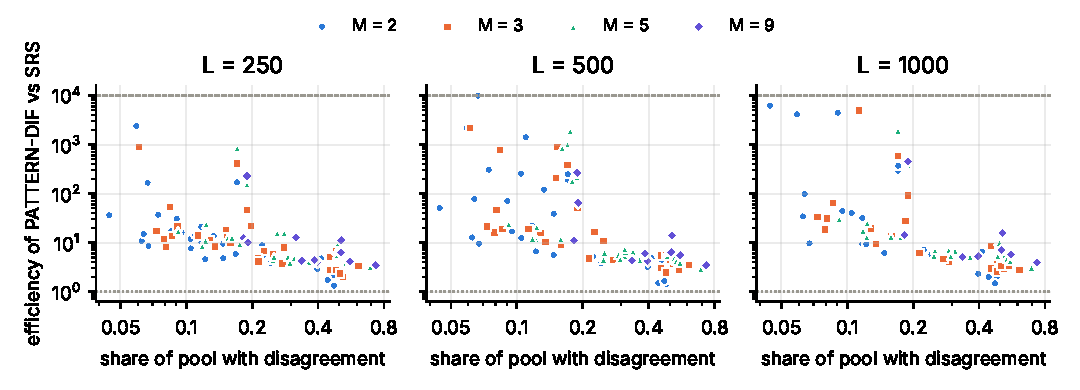
\includegraphics[width=\textwidth]{abl_dif_models_disagreement}
\caption{Efficiency of PATTERN-DIF relative to SRS (median over targets) against the share of the pool on which the compared models do not all agree, for random subsets of $M$ models in every setting (A3). Both axes are logarithmic; the dotted line marks parity and the dashed line the clipping value $10^4$.}
\label{fig:abl-models}
\end{figure*}

\subsection{Small-sample inference (A4)}

With the plain estimator the main study found worst-target coverage near 0.5 at $L=250$ in Churn and Law school, traced to strata whose sampled units show no variation in the influence values. The difference estimator removes most of this: the residual $\xi_i=t_i-\psi_i=(Y_i-\pi_i)(u_i-v_i)$ varies even when no positive is sampled, no (replication, target) pair had a standard error of exactly zero (plain estimator: up to 1.0\% in Law school), and the worst-target Wald coverage in Churn at $L=250$ rises from 0.47 to 0.91 (Table~\Mref{tab:abl-inference}, Figure~\ref{fig:abl-coverage}). The shortfalls that remain are of a different kind. Over the 29 cells the worst-target Wald coverage is below 0.85 in five cells (Law school 0.63, MAGIC 0.78 and Adult-sex 0.82 at $L=250$, Bank 0.83 and Phoneme 0.83 at $L=500$), against five cells for HT and six for SRS-DIF. The worst target is a TPR contrast in 17 of 29 cells (FPR in 4, error difference in 8). On average over cells its mean standard error is 0.90 of the Monte Carlo standard deviation (0.99 for the median target) and its bias is below 0.16 standard deviations, so the intervals are too short rather than off-centre, which is consistent with a linearisation error in a ratio with few sampled positives in the smaller group (we did not test this further).

None of the standard corrections closes this gap. A $t$ quantile with \citet{satterthwaite1946} degrees of freedom adds 1\% to the width and moves the mean worst target at $L=250$ from 0.852 to 0.865. The stratified bootstrap percentile interval \citep{efron1979}, which resamples labelled residuals within strata ($B=999$, no finite-population correction; \citealt{raowu1988} discuss a rescaled version), is 11\% wider and a little conservative (mean coverage 0.961 over all cells), with worst target 0.878 and minimum 0.767. The proxy variance floor of \texttt{tcs.labeling\_dif} replaces the sample variance of a stratum by its proxy residual variance when the former is exactly zero ('zero') or by the larger of the two in every stratum ('max'). The 'zero' floor leaves the width unchanged (1.002) and lifts the minimum over cells from 0.633 to 0.780, entirely through Law school (0.90 at $L=250$); combined with the $t$ quantile the mean worst target is 0.885 and four cells stay below 0.85. Only the 'max' floor reaches 0.92 in every cell (mean worst target 0.948), and it is conservative: mean coverage 0.985 at $L=250$, width 1.67 times Wald on average, 1.25 in the median and 4.9 in Law school. For SRS-DIF Wald coverage is poor (minimum 0.27) and the bootstrap worse (0.10); 'max' repairs it (minimum 0.88) at 23\% extra width. The floors were designed after seeing the failure of the plain estimator on these pools, so the 'zero' result for Law school is in-sample (the residual floor is discussed further in Section~\ref{sec:simulation}). An independent check on synthetic pools (\texttt{results/floor\_check.json}) found that the floor leaves the interval width unchanged (median ratio 1.00).

\begin{figure*}[t]
\centering
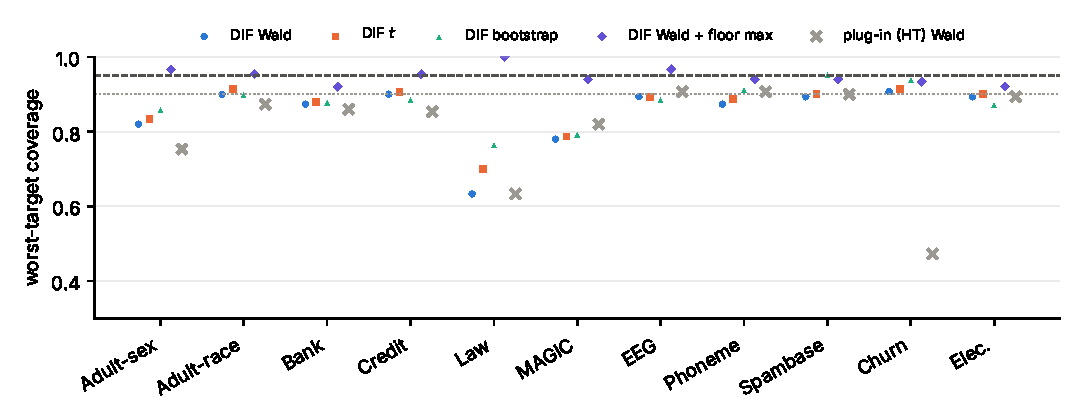
\includegraphics[width=\textwidth]{abl_dif_coverage_L250}
\caption{Worst-target coverage at $L=250$ in each setting for PATTERN-DIF under four interval methods and for the plain estimator (A4). Dashed line: nominal 0.95; dotted line: expected minimum over 108 targets of 150-replicate coverage if every target covered exactly 95\% (0.90; Law school has 57 targets).}
\label{fig:abl-coverage}
\end{figure*}

\subsection{Ranking models by the equalised-odds gap (A5)}

Practitioners also look at each model's equalised-odds gap $EO_m=\max(|\Delta^{TPR}_m|,|\Delta^{FPR}_m|)$ \citep{hardt2016} and rank models by it. We computed the plug-in $\widehat{EO}_m=f_{EO}(\hat T)$ from the totals of the same samples, with the difference estimator (DIF totals) and the plain estimator, and recorded the RMSE, the probability $P$ that the model with the smallest estimated gap has the smallest true gap, Kendall's $\tau$ \citep{kendall1938} between estimated and true gaps, and the bias. We also include a variant of PATTERN whose allocation targets the $2M$ per-model gaps instead of the comparison contrasts (gap-targeted). Table~\ref{tab:abl-eo} summarises the results; per-cell values are in Table~\ref{tab:abl-app-eo}.

The plug-in $\widehat{EO}_m$ is biased upwards, as a maximum of absolute values must be (mean bias 0.042 for SRS, 0.026 for PATTERN with HT, 0.024 for PATTERN-DIF, 0.019 for the gap-targeted variant with DIF). PATTERN-DIF is more accurate than SRS in the median (efficiency 1.94 to 2.21) and identifies the best model more often (mean $P$ 0.50 against 0.35 at $L=250$; 0.46 against 0.21 without Law school, where six models tie, and EEG, where the best model leads by 0.039). PATTERN with HT reaches efficiency 1.80 to 1.94 and $P$ 0.46 to 0.62, so the difference estimator adds little for this purpose. The gain is not uniform: PATTERN-DIF is less accurate than SRS in all Electricity cells (0.57 to 0.73) and in MAGIC at $L=1000$, because the allocation spends labels on disagreement whereas the gap of one model depends on all of its positive predictions. SRS-DIF has about the same RMSE efficiency (2.08 to 2.28) but a lower $P$ (0.42 at $L=250$) and $\tau$ (0.41). The gap-targeted allocation with the difference estimator is the best design here (efficiency 2.30 to 2.61, $P=0.49$, 0.56, 0.65 and $\tau=0.48$, 0.54, 0.64 by budget; never worse than SRS except in Law school) but it keeps only 74\% of the precision for the comparison contrasts (Table~\Mref{tab:abl-design}). In Law school the models are near-perfect and six have $EO_m=0$ exactly; the plain estimator then returns exactly zero for them and wins every tie, whereas the difference estimator does not (MSE ratio clipped at $10^{-4}$). When the true margin to the next model is 0.002 or less (Adult-sex, Bank, Credit card default, Churn) identification is hard for every design: $P$ for PATTERN-DIF is at most 0.55 at the largest budget and 0.11 in Credit card default (margin 0.0003).

\begin{table*}[t]
\centering\footnotesize
\setlength{\tabcolsep}{4pt}
\caption{Equalised-odds gap (A5). Eff.: median over cells of the median over models of $\mathrm{MSE}_{\mathrm{SRS}}/\mathrm{MSE}$ for $\widehat{EO}_m$ (cells in which both are exactly zero are skipped); $P$: mean probability that the estimated smallest-gap model has the smallest true gap; $\tau$: mean Kendall $\tau$ between estimated and true $EO_m$. DIF: totals from the difference estimator; plug-in: plain estimator.}
\label{tab:abl-eo}
\begin{tabular}{lccccccccc}
\toprule
 & \multicolumn{3}{c}{$L=250$} & \multicolumn{3}{c}{$L=500$} & \multicolumn{3}{c}{$L=1000$} \\
\cmidrule(lr){2-4}\cmidrule(lr){5-7}\cmidrule(lr){8-10}
Design & Eff. & $P$ & $\tau$ & Eff. & $P$ & $\tau$ & Eff. & $P$ & $\tau$ \\
\midrule
SRS (plug-in) & 1.00 & 0.35 & 0.32 & 1.00 & 0.42 & 0.39 & 1.00 & 0.49 & 0.48 \\
SRS-DIF (PPI) & 2.08 & 0.42 & 0.41 & 2.22 & 0.47 & 0.45 & 2.28 & 0.53 & 0.55 \\
GROUP, plug-in & 1.07 & 0.37 & 0.34 & 1.10 & 0.43 & 0.42 & 1.63 & 0.51 & 0.52 \\
PATTERN, plug-in (HT) & 1.83 & 0.46 & 0.45 & 1.80 & 0.51 & 0.49 & 1.94 & 0.62 & 0.62 \\
PATTERN-DIF (default) & 1.94 & 0.50 & 0.48 & 1.94 & 0.53 & 0.51 & 2.21 & 0.61 & 0.62 \\
Gap-targeted, plug-in & 2.03 & 0.44 & 0.43 & 2.29 & 0.52 & 0.51 & 2.54 & 0.59 & 0.61 \\
Gap-targeted, DIF & 2.30 & 0.49 & 0.48 & 2.61 & 0.56 & 0.54 & 2.51 & 0.65 & 0.64 \\
ORACLE-ALLOC, DIF & 2.02 & 0.50 & 0.47 & 1.77 & 0.54 & 0.52 & 1.93 & 0.57 & 0.60 \\
\bottomrule
\end{tabular}

\end{table*}

\paragraph{Summary.} With the difference estimator the ablation conclusions about the design are those of the earlier plug-in study: the count $K_i$ is the stratifier worth having, Neyman rather than proportional allocation matters, the allocation is insensitive to the proxy, and the gain depends on how often the compared models disagree. Three things differ. First, the proxy now matters in the estimator, where a poor proxy costs up to half of the efficiency and removes the advantage over HT, although coverage is unaffected; the ensemble mean was never beaten there. Second, the difference estimator removes the zero-variance failure of the plain estimator, so the proxy variance floor has become a cheap safeguard ('zero', no loss of width) rather than a 19\% widening, and the remaining undercoverage of rate contrasts at $L=250$ is not fixed by $t$ quantiles, the bootstrap or the floor; only the conservative 'max' floor reaches nominal worst-target coverage. Third, for ranking models by $EO_m$ itself the gap-targeted allocation with the difference estimator is better than the default. Neither tuned $\lambda$ nor proxy-bin strata beat the default consistently, and we keep it; we recommend reporting the Wald interval with the 'zero' floor, which costs nothing in width.

\section{Ablations: full tables}
\label{sec:app-ablations}\label{si:ablation-tables}

This appendix gives the per-cell results behind Section~\Mref{sec:ablations}: 29 setting--budget cells, $R=150$ replications and $B=999$ bootstrap resamples. All values are stored in
\path{results/label_ablations_dif.json}, which is produced by \path{experiments/label_ablations_dif.py}; its \texttt{report} mode (\path{experiments/label_ablations_dif_report.py}) writes the tables of this appendix and of Section~\Mref{sec:ablations} to \path{manuscript_v2/tables/} and draws the figures. Abbreviations: Credit = Credit card default, Law = Law school, Elec.\ = Electricity; DIF = stratified difference estimator with $\lambda=1$; HT = plain (expansion) estimator.

\paragraph{Implementation details.} Stratifiers: the binary stratifier crosses group with the indicator $0<K_i<M$. The three-model pattern uses the models with the highest agreement between $\hat y_{mi}$ and $\mathbf 1\{\pi_i\ge 0.5\}$ (chosen without labels), with the eight patterns ordered by their number of ones so that merging of small strata goes to a neighbouring pattern. Proxy bins split each $(G,K)$ cell at the quantiles of $\pi_i$ within the cell. All stratifiers merge strata below 50 units within group, as in the default; the default design has $H=6$ (Churn) to 20 (Electricity) strata. When $H$ strata at 10 labels would use more than 80\% of the budget, the floor is lowered to $\max(2,\lfloor 0.8L/H\rfloor)$; this affects only the proxy-bin stratifiers at $L\le 500$ (floors 3 to 9, in 14 cells for tertile bins). Proxies: ``single model'' uses the predicted probabilities of the first logistic regression (LR) or of Gaussian naive Bayes (NB); the constant proxy is 0.5; ``noise'' adds $N(0,2^2)$ to $\mathrm{logit}(\pi_i)$; ``shuffle'' permutes $\pi$ within each group (fixed seed); ``reversed'' is $1-\pi_i$; ``true labels'' uses $Y_i$ in the allocation only. A proxy $\tilde\pi$ in the estimator means $\psi_i=\tilde\pi_iu_i+(1-\tilde\pi_i)v_i$ in the difference estimator and, for the tuned weight, in $\lambda_{hk}$ of the stratified PPI estimator of \path{tcs/labeling_baselines.py} (clipped to $[0,1]$, estimated per stratum and target). Satterthwaite degrees of freedom are $\nu=(\sum_h a_h s^2_{e,h})^2/\sum_h (a_h s^2_{e,h})^2/(n_h-1)$ with $a_h=N_h^2(1-n_h/N_h)/n_h$ and $s^2_{e,h}$ the sample variance of the residual influence values, computed per target; for ``$t$ + floor'' the floored variances replace $s^2_{e,h}$ in both numerator and denominator. The bootstrap resamples the $n_h$ labelled units within each stratum with replacement, recomputes $T=\sum_Uf_i+\sum_hN_h\bar e^{*}_h$ with the pool-wide proxy total held fixed, and takes the 2.5\% and 97.5\% quantiles of the plug-in estimate. The two proxy variance floors are those of \path{tcs/labeling_dif.py}. A3 subsets were drawn once per size with seed 20261104 (the seed of the earlier study, so the subsets are identical). A5 computes $\widehat{EO}_m$ from the estimated totals (DIF totals for the difference estimator, expansion totals otherwise); the margin is the true $EO$ difference between the best model and the next model with a larger gap.

\begin{table*}[t]
\centering\scriptsize
\caption{Efficiency relative to SRS (median over live targets of $\mathrm{MSE}_{\mathrm{SRS}}/\mathrm{MSE}$, SRS with the plain estimator) for every cell and every stratifier (A1), difference estimator unless stated. Pat.: PATTERN-DIF (default); Pat.\ HT: the same sample with the plain estimator; Grp: GROUP; SRS: SRS-DIF; Bin.: group $\times$ agree/disagree; J3: three-model pattern; KP2, KP3: $K\times$ 2 or 3 proxy bins; Res.: residual allocation; Prop.: proportional allocation over the default strata.}
\label{tab:abl-app-eff-design}
\setlength{\tabcolsep}{3pt}
\begin{tabular}{lrrrrrrrrrrr}
\toprule
Setting & $L$ & Pat. & Pat.\ HT & Grp & SRS & Bin. & J3 & KP2 & KP3 & Res. & Prop. \\
\midrule
Adult-sex & 250 & 6.27 & 3.63 & 2.10 & 1.83 & 3.24 & 2.60 & 6.75 & 6.79 & 5.64 & 5.96 \\
Adult-sex & 500 & 6.38 & 3.90 & 2.02 & 2.01 & 3.47 & 3.46 & 6.71 & 6.34 & 6.33 & 4.64 \\
Adult-sex & 1000 & 7.04 & 4.48 & 2.05 & 1.90 & 3.58 & 3.56 & 7.80 & 7.45 & 7.27 & 3.75 \\
Adult-race & 250 & 11.18 & 6.02 & 3.43 & 1.82 & 5.51 & 4.39 & 12.31 & 11.09 & 11.80 & 10.66 \\
Adult-race & 500 & 13.90 & 6.30 & 3.61 & 1.70 & 5.89 & 4.41 & 12.18 & 10.35 & 12.98 & 6.83 \\
Adult-race & 1000 & 15.73 & 8.30 & 3.66 & 2.03 & 6.55 & 6.35 & 16.29 & 14.01 & 12.31 & 4.77 \\
Bank & 250 & 12.33 & 7.58 & 3.72 & 1.52 & 11.66 & 4.03 & 10.52 & 11.28 & 10.13 & 8.67 \\
Bank & 500 & 11.14 & 8.00 & 3.90 & 1.60 & 10.75 & 4.58 & 11.37 & 11.39 & 11.59 & 5.98 \\
Bank & 1000 & 14.44 & 9.85 & 4.10 & 1.65 & 15.00 & 4.77 & 15.26 & 15.34 & 13.26 & 3.90 \\
Credit & 250 & 4.15 & 2.83 & 2.00 & 1.76 & 2.75 & 2.92 & 4.42 & 4.74 & 4.31 & 4.33 \\
Credit & 500 & 5.48 & 3.97 & 1.67 & 1.74 & 2.45 & 3.13 & 5.00 & 4.44 & 5.18 & 4.27 \\
Credit & 1000 & 5.69 & 4.20 & 2.02 & 1.77 & 2.51 & 3.31 & 6.56 & 5.78 & 6.09 & 3.26 \\
Law & 250 & 227.66 & 15.71 & 22.01 & 10.85 & 147.87 & 21.67 & 327.79 & 325.04 & 246.06 & 106.46 \\
Law & 500 & 267.97 & 36.85 & 20.83 & 11.87 & 134.54 & 17.68 & 512.00 & 379.54 & 323.57 & 85.76 \\
Law & 1000 & 456.17 & 78.85 & 22.25 & 11.21 & 299.51 & 20.73 & $>$1000 & $>$1000 & 410.76 & 76.27 \\
MAGIC & 250 & 3.96 & 2.56 & 2.01 & 1.85 & 3.83 & 2.07 & 4.43 & 4.42 & 4.34 & 3.15 \\
MAGIC & 500 & 4.24 & 2.53 & 2.10 & 1.96 & 4.02 & 2.81 & 4.44 & 4.21 & 4.66 & 3.06 \\
MAGIC & 1000 & 5.30 & 3.15 & 1.95 & 2.01 & 5.24 & 2.61 & 5.76 & 5.54 & 5.99 & 2.72 \\
EEG & 250 & 3.47 & 1.72 & 2.17 & 1.93 & 2.50 & 2.48 & 3.85 & 4.06 & 3.39 & 3.10 \\
EEG & 500 & 3.44 & 1.75 & 1.95 & 1.93 & 2.50 & 2.55 & 3.65 & 3.49 & 3.13 & 2.61 \\
EEG & 1000 & 3.94 & 1.95 & 2.10 & 1.95 & 2.85 & 2.83 & 4.45 & 4.64 & 4.23 & 3.05 \\
Phoneme & 250 & 4.44 & 2.48 & 2.09 & 2.03 & 4.20 & 2.45 & 3.59 & 3.67 & 4.16 & 3.28 \\
Phoneme & 500 & 5.99 & 3.59 & 2.06 & 2.03 & 5.12 & 2.83 & 6.13 & 5.46 & 5.71 & 2.92 \\
Spambase & 250 & 12.75 & 5.55 & 2.88 & 2.12 & 11.77 & 3.46 & 9.37 & 7.00 & 13.20 & 3.60 \\
Churn & 250 & 10.13 & 6.51 & 1.55 & 1.50 & 9.38 & 2.82 & 8.22 & 7.59 & 9.42 & 3.35 \\
Churn & 500 & 65.20 & 31.59 & 1.67 & 1.55 & 48.70 & 2.78 & 37.77 & 26.93 & 32.61 & 2.93 \\
Elec. & 250 & 4.28 & 2.73 & 1.81 & 1.72 & 4.33 & 1.47 & 4.26 & 4.31 & 4.17 & 3.85 \\
Elec. & 500 & 4.29 & 2.82 & 1.77 & 1.90 & 4.17 & 2.13 & 4.40 & 4.03 & 4.63 & 3.23 \\
Elec. & 1000 & 5.09 & 3.37 & 1.80 & 1.87 & 4.39 & 2.14 & 4.83 & 4.96 & 4.82 & 2.42 \\
\bottomrule
\end{tabular}

\end{table*}

\begin{table*}[t]
\centering\scriptsize
\caption{Efficiency relative to SRS for every cell and allocation proxy (A2), with the same proxy in allocation and difference estimator (LR, NB, C = constant, Sh. = shuffled, Noi. = noise, Rev. = $1-\pi$). Orc.: allocation by the true labels, estimator with the ensemble proxy. Pat.: default.}
\label{tab:abl-app-eff-proxy}
\setlength{\tabcolsep}{4pt}
\begin{tabular}{lrrrrrrrrr}
\toprule
Setting & $L$ & Pat. & LR & NB & C & Sh. & Noi. & Rev. & Orc. \\
\midrule
Adult-sex & 250 & 6.27 & 5.81 & 3.64 & 4.46 & 2.57 & 2.91 & 4.19 & 5.94 \\
Adult-sex & 500 & 6.38 & 5.38 & 4.19 & 5.76 & 3.69 & 3.47 & 4.38 & 7.51 \\
Adult-sex & 1000 & 7.04 & 7.08 & 3.63 & 7.01 & 3.88 & 3.97 & 4.72 & 6.91 \\
Adult-race & 250 & 11.18 & 11.28 & 6.21 & 9.37 & 5.72 & 6.52 & 7.22 & 12.30 \\
Adult-race & 500 & 13.90 & 11.60 & 7.34 & 10.05 & 5.96 & 7.94 & 7.63 & 11.25 \\
Adult-race & 1000 & 15.73 & 14.73 & 7.72 & 10.60 & 8.22 & 9.50 & 7.37 & 17.39 \\
Bank & 250 & 12.33 & 9.51 & 6.72 & 9.35 & 3.74 & 3.26 & 6.88 & 10.39 \\
Bank & 500 & 11.14 & 12.33 & 8.01 & 10.53 & 5.13 & 4.57 & 8.01 & 12.32 \\
Bank & 1000 & 14.44 & 14.40 & 9.60 & 12.26 & 6.74 & 7.42 & 9.81 & 15.13 \\
Credit & 250 & 4.15 & 4.51 & 2.90 & 3.85 & 3.70 & 3.10 & 3.01 & 4.86 \\
Credit & 500 & 5.48 & 5.23 & 3.32 & 4.81 & 3.78 & 3.36 & 3.62 & 5.34 \\
Credit & 1000 & 5.69 & 5.56 & 3.88 & 5.71 & 4.26 & 4.00 & 4.88 & 6.01 \\
Law & 250 & 227.66 & 672.95 & 28.53 & 31.71 & 3.17 & 18.29 & 9.02 & 228.93 \\
Law & 500 & 267.97 & 794.02 & 36.52 & 47.31 & 4.85 & 20.28 & 11.45 & 262.24 \\
Law & 1000 & 456.17 & $>$1000 & 82.86 & 161.42 & 5.38 & 38.04 & 48.88 & 331.39 \\
MAGIC & 250 & 3.96 & 2.97 & 2.31 & 3.49 & 2.40 & 2.30 & 2.52 & 4.59 \\
MAGIC & 500 & 4.24 & 3.42 & 2.64 & 3.73 & 2.66 & 2.90 & 2.97 & 4.43 \\
MAGIC & 1000 & 5.30 & 4.43 & 3.28 & 4.72 & 2.93 & 3.25 & 3.23 & 5.51 \\
EEG & 250 & 3.47 & 2.42 & 1.55 & 2.82 & 1.94 & 1.55 & 1.74 & 3.32 \\
EEG & 500 & 3.44 & 2.29 & 1.49 & 2.64 & 1.77 & 1.73 & 1.69 & 3.46 \\
EEG & 1000 & 3.94 & 2.75 & 1.59 & 2.90 & 2.21 & 2.16 & 1.97 & 4.43 \\
Phoneme & 250 & 4.44 & 3.33 & 2.56 & 3.49 & 1.82 & 2.17 & 2.84 & 4.19 \\
Phoneme & 500 & 5.99 & 4.36 & 4.27 & 4.38 & 2.61 & 3.46 & 3.42 & 5.47 \\
Spambase & 250 & 12.75 & 10.07 & 8.62 & 9.20 & 4.60 & 6.92 & 5.19 & 14.59 \\
Churn & 250 & 10.13 & 6.07 & 5.94 & 9.07 & 4.71 & 6.38 & 6.39 & 10.21 \\
Churn & 500 & 65.20 & 70.28 & $>$1000 & $>$1000 & 255.08 & 68.66 & 37.93 & 60.60 \\
Elec. & 250 & 4.28 & 3.70 & 2.90 & 3.79 & 2.67 & 2.72 & 3.10 & 4.35 \\
Elec. & 500 & 4.29 & 3.59 & 3.18 & 4.15 & 2.82 & 2.96 & 3.17 & 4.19 \\
Elec. & 1000 & 5.09 & 4.70 & 3.46 & 4.57 & 3.25 & 3.46 & 3.83 & 5.03 \\
\bottomrule
\end{tabular}

\end{table*}

\begin{table*}[t]
\centering\scriptsize
\caption{As Table~\ref{tab:abl-app-eff-proxy} for the plain estimator (HT): the proxy enters the allocation only. Pat.: ensemble proxy.}
\label{tab:abl-app-eff-proxy-ht}
\setlength{\tabcolsep}{4pt}
\begin{tabular}{lrrrrrrrrr}
\toprule
Setting & $L$ & Pat. & LR & NB & C & Sh. & Noi. & Rev. & Orc. \\
\midrule
Adult-sex & 250 & 3.63 & 3.12 & 3.55 & 3.36 & 3.53 & 3.69 & 3.57 & 3.20 \\
Adult-sex & 500 & 3.90 & 3.79 & 4.05 & 3.97 & 3.86 & 3.89 & 3.99 & 3.69 \\
Adult-sex & 1000 & 4.48 & 4.33 & 4.28 & 4.30 & 4.14 & 4.40 & 4.28 & 4.50 \\
Adult-race & 250 & 6.02 & 6.01 & 5.69 & 5.58 & 5.30 & 5.67 & 6.32 & 5.87 \\
Adult-race & 500 & 6.30 & 6.06 & 6.54 & 5.94 & 5.96 & 6.78 & 6.08 & 6.33 \\
Adult-race & 1000 & 8.30 & 7.02 & 7.14 & 7.37 & 7.04 & 6.97 & 7.70 & 7.58 \\
Bank & 250 & 7.58 & 6.88 & 7.26 & 6.82 & 7.29 & 7.37 & 6.81 & 7.13 \\
Bank & 500 & 8.00 & 8.68 & 8.41 & 7.70 & 8.52 & 8.21 & 7.71 & 8.03 \\
Bank & 1000 & 9.85 & 10.31 & 10.57 & 8.73 & 8.50 & 9.65 & 10.65 & 10.31 \\
Credit & 250 & 2.83 & 3.08 & 3.13 & 2.95 & 3.20 & 3.49 & 3.08 & 3.06 \\
Credit & 500 & 3.97 & 3.96 & 4.00 & 3.70 & 3.95 & 4.05 & 3.27 & 3.71 \\
Credit & 1000 & 4.20 & 4.30 & 4.42 & 4.24 & 4.25 & 4.05 & 4.12 & 3.78 \\
Law & 250 & 15.71 & 19.71 & 19.82 & 18.07 & 21.84 & 15.26 & 17.50 & 25.35 \\
Law & 500 & 36.85 & 36.00 & 29.92 & 37.65 & 36.07 & 39.21 & 34.64 & 43.36 \\
Law & 1000 & 78.85 & 113.76 & 84.30 & 79.61 & 75.75 & 66.62 & 78.81 & 150.09 \\
MAGIC & 250 & 2.56 & 2.38 & 2.23 & 2.53 & 2.46 & 2.48 & 2.43 & 2.61 \\
MAGIC & 500 & 2.53 & 2.75 & 2.79 & 2.70 & 2.78 & 2.69 & 2.95 & 2.85 \\
MAGIC & 1000 & 3.15 & 3.25 & 3.37 & 3.40 & 3.36 & 3.17 & 3.20 & 3.37 \\
EEG & 250 & 1.72 & 1.71 & 1.66 & 1.67 & 1.66 & 1.73 & 1.56 & 1.79 \\
EEG & 500 & 1.75 & 1.82 & 1.66 & 1.67 & 1.70 & 1.67 & 1.72 & 1.84 \\
EEG & 1000 & 1.95 & 1.92 & 1.95 & 2.02 & 2.00 & 2.03 & 1.96 & 2.15 \\
Phoneme & 250 & 2.48 & 2.49 & 2.37 & 2.29 & 2.47 & 2.43 & 2.53 & 2.33 \\
Phoneme & 500 & 3.59 & 3.55 & 3.39 & 3.45 & 3.42 & 3.55 & 3.41 & 3.20 \\
Spambase & 250 & 5.55 & 5.83 & 6.37 & 5.14 & 5.25 & 5.69 & 5.75 & 5.87 \\
Churn & 250 & 6.51 & 6.32 & 11.01 & 7.45 & 7.12 & 6.65 & 6.45 & 6.53 \\
Churn & 500 & 31.59 & 59.30 & $>$1000 & $>$1000 & 312.39 & 53.69 & 31.05 & 53.34 \\
Elec. & 250 & 2.73 & 2.65 & 2.81 & 2.81 & 2.75 & 2.83 & 2.67 & 2.75 \\
Elec. & 500 & 2.82 & 2.77 & 3.01 & 2.83 & 2.65 & 2.97 & 2.89 & 2.85 \\
Elec. & 1000 & 3.37 & 3.30 & 3.24 & 3.18 & 3.12 & 3.34 & 3.12 & 3.00 \\
\bottomrule
\end{tabular}

\end{table*}

\begin{table*}[t]
\centering\scriptsize
\caption{Tuned weight $\lambda$ (A2), efficiency relative to SRS for every cell. $\lambda=1$: default; tuned: $\lambda$ chosen per stratum and target on the labelled units; C, Sh., Rev.: constant, shuffled and reversed proxy with tuned $\lambda$; SRS $\lambda{=}1$ and SRS tuned: one stratum (PPI and PPI++ with the ensemble proxy).}
\label{tab:abl-app-eff-tuned}
\setlength{\tabcolsep}{4pt}
\begin{tabular}{lrrrrrrrr}
\toprule
Setting & $L$ & $\lambda=1$ & tuned & C tuned & Sh. tuned & Rev. tuned & SRS $\lambda$=1 & SRS tuned \\
\midrule
Adult-sex & 250 & 6.27 & 7.46 & 5.83 & 5.20 & 5.41 & 1.83 & 2.05 \\
Adult-sex & 500 & 6.38 & 6.47 & 6.84 & 5.86 & 5.64 & 2.01 & 2.18 \\
Adult-sex & 1000 & 7.04 & 7.26 & 7.08 & 5.88 & 5.84 & 1.90 & 2.00 \\
Adult-race & 250 & 11.18 & 12.86 & 10.44 & 9.90 & 8.07 & 1.82 & 2.51 \\
Adult-race & 500 & 13.90 & 14.37 & 11.72 & 9.73 & 9.06 & 1.70 & 2.03 \\
Adult-race & 1000 & 15.73 & 16.60 & 11.27 & 10.12 & 8.54 & 2.03 & 2.16 \\
Bank & 250 & 12.33 & 13.14 & 10.41 & 8.27 & 10.01 & 1.52 & 2.15 \\
Bank & 500 & 11.14 & 11.51 & 10.93 & 10.04 & 10.79 & 1.60 & 1.95 \\
Bank & 1000 & 14.44 & 14.26 & 13.47 & 9.27 & 14.16 & 1.65 & 1.82 \\
Credit & 250 & 4.15 & 4.79 & 4.49 & 4.63 & 4.42 & 1.76 & 1.86 \\
Credit & 500 & 5.48 & 5.47 & 4.79 & 4.83 & 4.48 & 1.74 & 1.80 \\
Credit & 1000 & 5.69 & 5.85 & 5.84 & 5.09 & 5.40 & 1.77 & 1.78 \\
Law & 250 & 227.66 & 268.17 & 65.97 & 29.97 & 26.70 & 10.85 & 10.77 \\
Law & 500 & 267.97 & 240.23 & 106.40 & 43.99 & 35.00 & 11.87 & 11.90 \\
Law & 1000 & 456.17 & 429.49 & 313.84 & 98.94 & 102.98 & 11.21 & 11.21 \\
MAGIC & 250 & 3.96 & 4.00 & 3.81 & 3.26 & 3.36 & 1.85 & 1.98 \\
MAGIC & 500 & 4.24 & 4.33 & 3.96 & 3.39 & 4.03 & 1.96 & 2.00 \\
MAGIC & 1000 & 5.30 & 5.45 & 5.35 & 4.34 & 4.36 & 2.01 & 2.01 \\
EEG & 250 & 3.47 & 3.73 & 3.54 & 2.73 & 2.54 & 1.93 & 2.07 \\
EEG & 500 & 3.44 & 3.56 & 3.18 & 2.56 & 2.47 & 1.93 & 2.02 \\
EEG & 1000 & 3.94 & 4.14 & 3.31 & 3.28 & 2.99 & 1.95 & 2.04 \\
Phoneme & 250 & 4.44 & 4.23 & 3.96 & 2.99 & 3.48 & 2.03 & 2.01 \\
Phoneme & 500 & 5.99 & 6.06 & 4.61 & 4.25 & 4.30 & 2.03 & 2.03 \\
Spambase & 250 & 12.75 & 12.91 & 9.93 & 7.41 & 8.19 & 2.12 & 2.35 \\
Churn & 250 & 10.13 & 11.19 & 10.91 & 9.83 & 8.74 & 1.50 & 1.73 \\
Churn & 500 & 65.20 & 68.21 & $>$1000 & 431.21 & 45.99 & 1.55 & 1.67 \\
Elec. & 250 & 4.28 & 4.19 & 4.15 & 3.48 & 3.56 & 1.72 & 1.83 \\
Elec. & 500 & 4.29 & 4.39 & 4.39 & 3.37 & 3.75 & 1.90 & 1.95 \\
Elec. & 1000 & 5.09 & 5.20 & 4.57 & 4.05 & 4.55 & 1.87 & 1.92 \\
\bottomrule
\end{tabular}

\end{table*}

\begin{table*}[t]
\centering\scriptsize
\caption{Coverage of PATTERN-DIF per cell (A4). $H$: number of strata after merging. Mean: Wald coverage averaged over targets; the remaining coverage columns give the worst target under Wald, with the 'zero' floor, with the 'max' floor, with $t$ (Satterthwaite) and with the stratified bootstrap. Last two columns: worst-target coverage of PATTERN with the plain estimator and of SRS-DIF, both Wald. The Monte Carlo reference for the worst of 108 targets at exact 95\% coverage is 0.90 (57 targets in Law school).}
\label{tab:abl-app-cov}
\setlength{\tabcolsep}{4pt}
\begin{tabular}{lrrrrrrrrrr}
\toprule
 & & & & \multicolumn{5}{c}{Worst target, PATTERN-DIF} & \multicolumn{2}{c}{Worst, other} \\
\cmidrule(lr){5-9}\cmidrule(lr){10-11}
Setting & $L$ & $H$ & Mean & Wald & Zero & Max & $t$ & Boot. & HT & SRS-DIF \\
\midrule
Adult-sex & 250 & 19 & 0.946 & 0.820 & 0.820 & 0.967 & 0.833 & 0.860 & 0.753 & 0.913 \\
Adult-sex & 500 & 19 & 0.946 & 0.880 & 0.880 & 0.920 & 0.880 & 0.900 & 0.880 & 0.907 \\
Adult-sex & 1000 & 19 & 0.947 & 0.873 & 0.873 & 0.920 & 0.873 & 0.887 & 0.873 & 0.880 \\
Adult-race & 250 & 17 & 0.951 & 0.900 & 0.900 & 0.953 & 0.913 & 0.900 & 0.873 & 0.913 \\
Adult-race & 500 & 17 & 0.954 & 0.893 & 0.907 & 0.947 & 0.893 & 0.887 & 0.907 & 0.900 \\
Adult-race & 1000 & 17 & 0.949 & 0.913 & 0.913 & 0.927 & 0.920 & 0.933 & 0.913 & 0.907 \\
Bank & 250 & 16 & 0.942 & 0.873 & 0.873 & 0.920 & 0.880 & 0.880 & 0.860 & 0.900 \\
Bank & 500 & 16 & 0.939 & 0.833 & 0.833 & 0.927 & 0.833 & 0.860 & 0.860 & 0.900 \\
Bank & 1000 & 16 & 0.948 & 0.907 & 0.907 & 0.927 & 0.907 & 0.933 & 0.900 & 0.900 \\
Credit & 250 & 19 & 0.947 & 0.900 & 0.900 & 0.953 & 0.907 & 0.887 & 0.853 & 0.753 \\
Credit & 500 & 19 & 0.957 & 0.913 & 0.920 & 0.940 & 0.913 & 0.907 & 0.913 & 0.907 \\
Credit & 1000 & 19 & 0.946 & 0.907 & 0.907 & 0.933 & 0.907 & 0.933 & 0.913 & 0.907 \\
Law & 250 & 10 & 0.898 & 0.633 & 0.900 & 1.000 & 0.700 & 0.767 & 0.633 & 0.267 \\
Law & 500 & 10 & 0.951 & 0.933 & 0.933 & 1.000 & 0.933 & 0.953 & 0.920 & 0.400 \\
Law & 1000 & 10 & 0.945 & 0.907 & 0.907 & 0.987 & 0.913 & 0.953 & 0.900 & 0.640 \\
MAGIC & 250 & 19 & 0.935 & 0.780 & 0.780 & 0.940 & 0.787 & 0.793 & 0.820 & 0.833 \\
MAGIC & 500 & 19 & 0.933 & 0.887 & 0.887 & 0.940 & 0.887 & 0.900 & 0.880 & 0.913 \\
MAGIC & 1000 & 19 & 0.947 & 0.900 & 0.900 & 0.947 & 0.900 & 0.920 & 0.887 & 0.900 \\
EEG & 250 & 18 & 0.947 & 0.893 & 0.893 & 0.967 & 0.893 & 0.887 & 0.907 & 0.887 \\
EEG & 500 & 18 & 0.950 & 0.907 & 0.907 & 0.933 & 0.907 & 0.920 & 0.907 & 0.920 \\
EEG & 1000 & 18 & 0.949 & 0.887 & 0.887 & 0.927 & 0.887 & 0.927 & 0.900 & 0.893 \\
Phoneme & 250 & 14 & 0.947 & 0.873 & 0.873 & 0.940 & 0.887 & 0.913 & 0.907 & 0.913 \\
Phoneme & 500 & 14 & 0.945 & 0.833 & 0.833 & 0.940 & 0.833 & 0.927 & 0.900 & 0.893 \\
Spambase & 250 & 9 & 0.945 & 0.893 & 0.893 & 0.940 & 0.900 & 0.953 & 0.900 & 0.840 \\
Churn & 250 & 6 & 0.946 & 0.907 & 0.907 & 0.933 & 0.913 & 0.940 & 0.473 & 0.880 \\
Churn & 500 & 6 & 0.940 & 0.880 & 0.880 & 0.927 & 0.880 & 0.953 & 0.800 & 0.900 \\
Elec. & 250 & 20 & 0.948 & 0.893 & 0.893 & 0.920 & 0.900 & 0.873 & 0.893 & 0.893 \\
Elec. & 500 & 20 & 0.944 & 0.893 & 0.893 & 0.927 & 0.900 & 0.907 & 0.860 & 0.907 \\
Elec. & 1000 & 20 & 0.950 & 0.907 & 0.907 & 0.933 & 0.907 & 0.920 & 0.900 & 0.900 \\
\bottomrule
\end{tabular}

\end{table*}

\begin{table*}[t]
\centering\scriptsize
\caption{Average interval width relative to Wald for PATTERN-DIF per cell (A4), over replications and targets: 'zero' and 'max' floors, $t$ with Satterthwaite degrees of freedom, and stratified bootstrap percentile.}
\label{tab:abl-app-width}
\setlength{\tabcolsep}{6pt}
\begin{tabular}{lrrrrr}
\toprule
Setting & $L$ & Zero & Max & $t$ & Boot. \\
\midrule
Adult-sex & 250 & 1.005 & 1.45 & 1.03 & 1.01 \\
Adult-sex & 500 & 1.003 & 1.33 & 1.01 & 1.03 \\
Adult-sex & 1000 & 1.001 & 1.27 & 1.00 & 1.07 \\
Adult-race & 250 & 1.005 & 1.32 & 1.02 & 1.02 \\
Adult-race & 500 & 1.002 & 1.25 & 1.01 & 1.06 \\
Adult-race & 1000 & 1.001 & 1.22 & 1.00 & 1.14 \\
Bank & 250 & 1.001 & 1.33 & 1.02 & 1.10 \\
Bank & 500 & 1.000 & 1.25 & 1.01 & 1.10 \\
Bank & 1000 & 1.000 & 1.18 & 1.00 & 1.20 \\
Credit & 250 & 1.008 & 1.24 & 1.02 & 1.02 \\
Credit & 500 & 1.003 & 1.13 & 1.01 & 1.04 \\
Credit & 1000 & 1.001 & 1.10 & 1.00 & 1.08 \\
Law & 250 & 1.018 & 4.90 & 1.02 & 1.05 \\
Law & 500 & 1.002 & 4.85 & 1.01 & 1.15 \\
Law & 1000 & 1.000 & 4.89 & 1.01 & 1.40 \\
MAGIC & 250 & 1.003 & 1.25 & 1.02 & 1.00 \\
MAGIC & 500 & 1.001 & 1.19 & 1.01 & 1.05 \\
MAGIC & 1000 & 1.000 & 1.17 & 1.00 & 1.14 \\
EEG & 250 & 1.004 & 1.53 & 1.01 & 0.99 \\
EEG & 500 & 1.001 & 1.53 & 1.00 & 1.04 \\
EEG & 1000 & 1.000 & 1.53 & 1.00 & 1.12 \\
Phoneme & 250 & 1.001 & 1.19 & 1.01 & 1.11 \\
Phoneme & 500 & 1.000 & 1.19 & 1.01 & 1.32 \\
Spambase & 250 & 1.002 & 1.37 & 1.01 & 1.31 \\
Churn & 250 & 1.000 & 1.78 & 1.01 & 1.14 \\
Churn & 500 & 1.000 & 1.64 & 1.01 & 1.42 \\
Elec. & 250 & 1.003 & 1.15 & 1.01 & 0.99 \\
Elec. & 500 & 1.001 & 1.12 & 1.01 & 1.03 \\
Elec. & 1000 & 1.000 & 1.10 & 1.00 & 1.10 \\
\bottomrule
\end{tabular}

\end{table*}

\begin{table*}[t]
\centering\scriptsize
\caption{Equalised-odds gaps per cell (A5). Margin: true $EO$ gap between the best and the next distinct model (in Law school six models tie at $EO_m=0$, so the plain estimator, which returns exactly zero for them, wins every tie). $P(\mathrm{best})$: probability that the estimated smallest-gap model has the smallest true gap for SRS, PATTERN with the plain estimator (HT), PATTERN-DIF (DIF) and the gap-targeted allocation with DIF (Gap-DIF). Kendall $\tau$ for SRS and PATTERN-DIF. Eff.: median over models of $\mathrm{MSE}_{\mathrm{SRS}}/\mathrm{MSE}$ of $\widehat{EO}_m$ for PATTERN-DIF.}
\label{tab:abl-app-eo}
\setlength{\tabcolsep}{4pt}
\begin{tabular}{lrrrrrrrrrr}
\toprule
 & & & & \multicolumn{4}{c}{$P(\mathrm{best})$} & \multicolumn{2}{c}{Kendall $\tau$} & Eff. \\
\cmidrule(lr){5-8}\cmidrule(lr){9-10}
Setting & $L$ & Margin & Ties & SRS & HT & DIF & Gap-DIF & SRS & DIF & DIF \\
\midrule
Adult-sex & 250 & 0.002 & 1 & 0.19 & 0.29 & 0.43 & 0.42 & 0.06 & 0.34 & 2.29 \\
Adult-sex & 500 & 0.002 & 1 & 0.27 & 0.33 & 0.45 & 0.59 & 0.20 & 0.48 & 2.56 \\
Adult-sex & 1000 & 0.002 & 1 & 0.32 & 0.48 & 0.55 & 0.57 & 0.30 & 0.61 & 2.27 \\
Adult-race & 250 & 0.025 & 1 & 0.13 & 0.27 & 0.39 & 0.35 & 0.03 & 0.25 & 7.30 \\
Adult-race & 500 & 0.025 & 1 & 0.18 & 0.37 & 0.42 & 0.45 & 0.09 & 0.36 & 6.00 \\
Adult-race & 1000 & 0.025 & 1 & 0.22 & 0.57 & 0.63 & 0.72 & 0.14 & 0.52 & 3.41 \\
Bank & 250 & 0.002 & 1 & 0.11 & 0.20 & 0.29 & 0.23 & 0.01 & 0.18 & 3.62 \\
Bank & 500 & 0.002 & 1 & 0.17 & 0.27 & 0.32 & 0.30 & 0.10 & 0.16 & 2.95 \\
Bank & 1000 & 0.002 & 1 & 0.12 & 0.40 & 0.48 & 0.43 & 0.11 & 0.32 & 3.44 \\
Credit & 250 & 0.000 & 1 & 0.15 & 0.11 & 0.15 & 0.10 & 0.05 & 0.26 & 1.04 \\
Credit & 500 & 0.000 & 1 & 0.16 & 0.13 & 0.13 & 0.13 & 0.07 & 0.24 & 1.37 \\
Credit & 1000 & 0.000 & 1 & 0.10 & 0.13 & 0.11 & 0.17 & 0.09 & 0.21 & 2.15 \\
Law & 250 & 0.002 & 6 & 1.00 & 1.00 & 0.45 & 0.58 & 0.87 & 0.68 & 0.00 \\
Law & 500 & 0.002 & 6 & 1.00 & 1.00 & 0.49 & 0.49 & 0.90 & 0.71 & 0.00 \\
Law & 1000 & 0.002 & 6 & 1.00 & 1.00 & 0.59 & 0.63 & 0.94 & 0.76 & 0.00 \\
MAGIC & 250 & 0.008 & 1 & 0.17 & 0.39 & 0.55 & 0.55 & 0.40 & 0.53 & 1.03 \\
MAGIC & 500 & 0.008 & 1 & 0.29 & 0.56 & 0.73 & 0.79 & 0.49 & 0.63 & 1.19 \\
MAGIC & 1000 & 0.008 & 1 & 0.57 & 0.76 & 0.84 & 0.91 & 0.60 & 0.75 & 0.95 \\
EEG & 250 & 0.039 & 1 & 1.00 & 0.99 & 1.00 & 1.00 & 0.64 & 0.73 & 2.69 \\
EEG & 500 & 0.039 & 1 & 0.98 & 1.00 & 1.00 & 1.00 & 0.74 & 0.83 & 2.52 \\
EEG & 1000 & 0.039 & 1 & 1.00 & 1.00 & 1.00 & 1.00 & 0.80 & 0.90 & 2.63 \\
Phoneme & 250 & 0.027 & 1 & 0.28 & 0.46 & 0.59 & 0.59 & 0.45 & 0.57 & 1.94 \\
Phoneme & 500 & 0.027 & 1 & 0.47 & 0.51 & 0.65 & 0.68 & 0.53 & 0.65 & 1.32 \\
Spambase & 250 & 0.027 & 1 & 0.31 & 0.76 & 0.88 & 0.79 & 0.35 & 0.84 & 1.94 \\
Churn & 250 & 0.002 & 1 & 0.17 & 0.29 & 0.46 & 0.34 & 0.04 & 0.14 & 4.94 \\
Churn & 500 & 0.002 & 1 & 0.17 & 0.45 & 0.53 & 0.59 & 0.06 & 0.23 & 2.85 \\
Elec. & 250 & 0.007 & 1 & 0.35 & 0.35 & 0.37 & 0.48 & 0.62 & 0.74 & 0.73 \\
Elec. & 500 & 0.007 & 1 & 0.46 & 0.49 & 0.58 & 0.60 & 0.77 & 0.82 & 0.66 \\
Elec. & 1000 & 0.007 & 1 & 0.57 & 0.59 & 0.65 & 0.73 & 0.83 & 0.92 & 0.57 \\
\bottomrule
\end{tabular}

\end{table*}

\begin{table*}[t]
\centering\scriptsize
\caption{Model subsets (A3) at $L=250$: for each of the nine random subsets (three of each size $M$, in the order drawn) the share of the pool on which the subset's models do not all agree and the median-over-targets efficiency of PATTERN-DIF relative to SRS, written as share/efficiency. ``exact'': the subset's models agree on every instance, so every target is zero and the subset is dropped. The last column is the full set of nine models.}
\label{tab:abl-app-models}
\setlength{\tabcolsep}{3pt}
\resizebox{\textwidth}{!}{\begin{tabular}{lcccc}
\toprule
Setting & $M=2$ & $M=3$ & $M=5$ & $M=9$ \\
\midrule
Adult-sex & 0.06/10.8, 0.40/2.9, 0.46/2.4 & 0.45/2.8, 0.48/2.7, 0.08/11.6 & 0.49/6.7, 0.49/5.8, 0.12/11.1 & 0.51/6.3 \\
Adult-race & 0.06/15.1, 0.41/4.8, 0.46/4.9 & 0.45/5.1, 0.48/7.0, 0.08/8.2 & 0.49/12.0, 0.50/10.0, 0.12/24.3 & 0.51/11.2 \\
Bank & 0.07/8.5, 0.12/21.1, 0.12/10.0 & 0.13/11.4, 0.14/8.3, 0.07/17.0 & 0.16/12.6, 0.18/9.4, 0.09/17.3 & 0.18/12.3 \\
Credit & 0.04/36.2, 0.47/2.2, 0.48/1.4 & 0.52/2.0, 0.50/2.3, 0.09/13.5 & 0.53/4.1, 0.54/3.9, 0.12/8.5 & 0.56/4.2 \\
Law & 0.06/2386.8, 0.17/166.5, 0.17/169.5 & 0.17/410.7, 0.19/46.2, exact & 0.17/854.4, 0.19/154.5, exact & 0.19/227.7 \\
MAGIC & 0.10/7.6, 0.22/5.4, 0.24/3.9 & 0.29/4.1, 0.27/3.8, 0.11/14.0 & 0.36/4.0, 0.31/5.3, 0.29/5.1 & 0.40/4.0 \\
EEG & 0.09/30.6, 0.44/1.7, 0.47/1.3 & 0.55/3.3, 0.61/3.3, 0.18/10.3 & 0.69/3.2, 0.56/4.0, 0.56/3.8 & 0.73/3.5 \\
Phoneme & 0.07/37.0, 0.13/13.7, 0.15/9.5 & 0.25/5.9, 0.23/6.7, 0.15/17.9 & 0.31/4.7, 0.31/4.8, 0.34/4.4 & 0.39/4.4 \\
Spambase & 0.09/17.1, 0.17/5.8, 0.22/8.9 & 0.20/21.8, 0.28/7.9, 0.09/21.2 & 0.26/15.8, 0.28/15.8, 0.15/12.5 & 0.32/12.7 \\
Churn & 0.10/11.9, 0.11/14.3, 0.07/166.7 & 0.15/12.7, 0.08/53.8, 0.06/878.6 & 0.18/12.5, 0.18/12.3, 0.16/12.6 & 0.19/10.1 \\
Elec. & 0.10/16.2, 0.15/4.8, 0.12/4.6 & 0.21/4.8, 0.21/4.1, 0.16/9.9 & 0.25/4.5, 0.30/3.9, 0.25/5.2 & 0.34/4.3 \\
\bottomrule
\end{tabular}
}
\end{table*}

\begin{table*}[t]
\centering\scriptsize
\setlength{\tabcolsep}{4pt}
\caption{The weight $\lambda$ (A2). Eff.: median over cells of efficiency vs SRS with the plain estimator; mean and worst: mean coverage and worst-target coverage, averaged over cells. The proxy named in the row is used in the allocation and, for $\lambda>0$, in the estimator; $\lambda$ tuned is chosen per stratum and target and clipped to $[0,1]$.}
\label{tab:abl-lambda}
\begin{tabular}{lccccccccc}
\toprule
 & \multicolumn{3}{c}{$\lambda=0$ (HT)} & \multicolumn{3}{c}{$\lambda=1$ (DIF)} & \multicolumn{3}{c}{$\lambda$ tuned} \\
\cmidrule(lr){2-4}\cmidrule(lr){5-7}\cmidrule(lr){8-10}
Proxy and design & Eff. & mean & worst & Eff. & mean & worst & Eff. & mean & worst \\
\midrule
Ensemble $\pi$, PATTERN & 3.97 & 0.944 & 0.858 & 6.27 & 0.945 & 0.877 & 6.47 & 0.923 & 0.799 \\
Ensemble $\pi$, SRS & 1.00 & 0.921 & 0.675 & 1.90 & 0.938 & 0.844 & 2.01 & 0.926 & 0.701 \\
Constant 0.5, PATTERN & 3.97 & 0.940 & 0.850 & 5.71 & 0.940 & 0.858 & 5.84 & 0.934 & 0.823 \\
Shuffled $\pi$, PATTERN & 3.95 & 0.940 & 0.854 & 3.70 & 0.949 & 0.889 & 5.20 & 0.924 & 0.783 \\
Noisy $\pi$, PATTERN & 4.05 & 0.943 & 0.854 & 3.46 & 0.949 & 0.877 & 5.07 & 0.923 & 0.806 \\
Reversed $1-\pi$, PATTERN & 3.99 & 0.942 & 0.859 & 4.38 & 0.941 & 0.872 & 5.41 & 0.932 & 0.835 \\
\bottomrule
\end{tabular}

\end{table*}

\begin{figure*}[t]
\centering
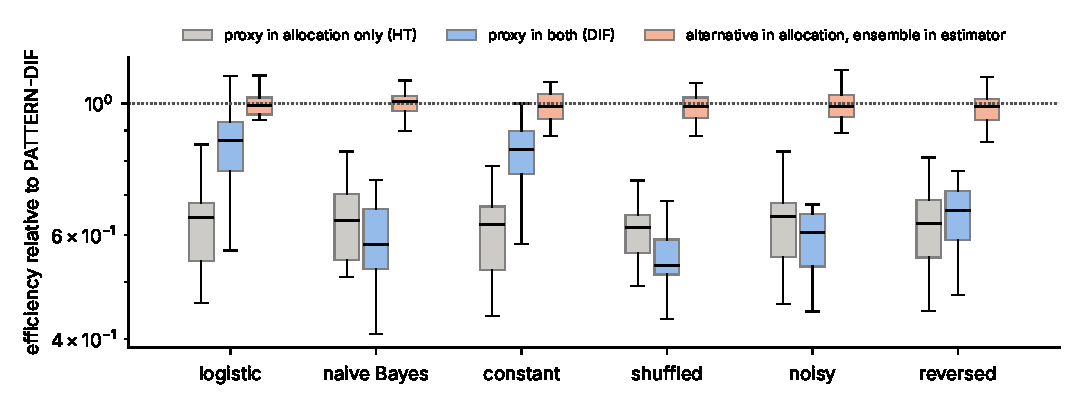
\includegraphics[width=0.95\textwidth]{abl_dif_proxy}
\caption{Efficiency of alternative proxies relative to PATTERN-DIF with the ensemble proxy (Rel.), one value per cell (29 cells; boxes: quartiles, whiskers: 1.5 interquartile ranges). Grey: proxy in the allocation only, plain estimator; blue: proxy in allocation and estimator; orange: proxy in the allocation only, difference estimator with the ensemble proxy.}
\label{fig:abl-proxy}
\end{figure*}

\section{Data sets and models}\label{app:data}

All data sets were obtained from OpenML through scikit-learn's \texttt{fetch\_openml} interface. Adult (version 2, 48,842 records; target income above 50K; groups: sex, female versus male, and race, non-White versus White); Bank Marketing (version 1, 45,211 records; target subscription; group: age below 30); default of credit card clients (version 1, 30,000 records; target default; group: sex); law school admission (binarised version, 20,800 records; group: race, non-White versus White); MAGIC gamma telescope (19,020 records); EEG eye state (14,980 records); Phoneme (5,404 records); Spambase (4,601 records); Churn (5,000 records); Electricity (45,312 records, subsampled to 30,000). For the last six the group is the indicator that the first numeric feature exceeds its median, and the feature is removed from the inputs. In all data sets the minority class is the positive class; for Adult, Bank Marketing and credit-card default this coincides with the conventional positive class (income above 50K, subscription, default).

Each data set was split once, stratified by the label, into a training part (60\%) and a pool (40\%), with seed 0. Numeric features were standardised and categorical features one-hot encoded inside each model's pipeline. The nine models are: logistic regression (default, and with inverse regularisation strength 0.01), decision trees of depth 3 and 12, a random forest with 200 trees and minimum leaf size 3, histogram gradient boosting with default settings, 25-nearest neighbours, Gaussian naive Bayes, and a multilayer perceptron with hidden layers of 64 and 32 units and early stopping. Pool predictions, predicted probabilities, group indicators and labels are cached by \texttt{experiments/preference\_validation.py} and used by all experiments.

\bibliography{references}
\end{document}
